\documentclass[twoside]{book}

% Packages required by doxygen
\usepackage{fixltx2e}
\usepackage{calc}
\usepackage{doxygen}
\usepackage[export]{adjustbox} % also loads graphicx
\usepackage{graphicx}
\usepackage[utf8]{inputenc}
\usepackage{makeidx}
\usepackage{multicol}
\usepackage{multirow}
\PassOptionsToPackage{warn}{textcomp}
\usepackage{textcomp}
\usepackage[nointegrals]{wasysym}
\usepackage[table]{xcolor}

% Font selection
\usepackage[T1]{fontenc}
\usepackage[scaled=.90]{helvet}
\usepackage{courier}
\usepackage{amssymb}
\usepackage{sectsty}
\renewcommand{\familydefault}{\sfdefault}
\allsectionsfont{%
  \fontseries{bc}\selectfont%
  \color{darkgray}%
}
\renewcommand{\DoxyLabelFont}{%
  \fontseries{bc}\selectfont%
  \color{darkgray}%
}
\newcommand{\+}{\discretionary{\mbox{\scriptsize$\hookleftarrow$}}{}{}}

% Page & text layout
\usepackage{geometry}
\geometry{%
  a4paper,%
  top=2.5cm,%
  bottom=2.5cm,%
  left=2.5cm,%
  right=2.5cm%
}
\tolerance=750
\hfuzz=15pt
\hbadness=750
\setlength{\emergencystretch}{15pt}
\setlength{\parindent}{0cm}
\setlength{\parskip}{3ex plus 2ex minus 2ex}
\makeatletter
\renewcommand{\paragraph}{%
  \@startsection{paragraph}{4}{0ex}{-1.0ex}{1.0ex}{%
    \normalfont\normalsize\bfseries\SS@parafont%
  }%
}
\renewcommand{\subparagraph}{%
  \@startsection{subparagraph}{5}{0ex}{-1.0ex}{1.0ex}{%
    \normalfont\normalsize\bfseries\SS@subparafont%
  }%
}
\makeatother

% Headers & footers
\usepackage{fancyhdr}
\pagestyle{fancyplain}
\fancyhead[LE]{\fancyplain{}{\bfseries\thepage}}
\fancyhead[CE]{\fancyplain{}{}}
\fancyhead[RE]{\fancyplain{}{\bfseries\leftmark}}
\fancyhead[LO]{\fancyplain{}{\bfseries\rightmark}}
\fancyhead[CO]{\fancyplain{}{}}
\fancyhead[RO]{\fancyplain{}{\bfseries\thepage}}
\fancyfoot[LE]{\fancyplain{}{}}
\fancyfoot[CE]{\fancyplain{}{}}
\fancyfoot[RE]{\fancyplain{}{\bfseries\scriptsize Generated by Doxygen }}
\fancyfoot[LO]{\fancyplain{}{\bfseries\scriptsize Generated by Doxygen }}
\fancyfoot[CO]{\fancyplain{}{}}
\fancyfoot[RO]{\fancyplain{}{}}
\renewcommand{\footrulewidth}{0.4pt}
\renewcommand{\chaptermark}[1]{%
  \markboth{#1}{}%
}
\renewcommand{\sectionmark}[1]{%
  \markright{\thesection\ #1}%
}

% Indices & bibliography
\usepackage{natbib}
\usepackage[titles]{tocloft}
\setcounter{tocdepth}{3}
\setcounter{secnumdepth}{5}
\makeindex

% Hyperlinks (required, but should be loaded last)
\usepackage{ifpdf}
\ifpdf
  \usepackage[pdftex,pagebackref=true]{hyperref}
\else
  \usepackage[ps2pdf,pagebackref=true]{hyperref}
\fi
\hypersetup{%
  colorlinks=true,%
  linkcolor=blue,%
  citecolor=blue,%
  unicode%
}

% Custom commands
\newcommand{\clearemptydoublepage}{%
  \newpage{\pagestyle{empty}\cleardoublepage}%
}

\usepackage{caption}
\captionsetup{labelsep=space,justification=centering,font={bf},singlelinecheck=off,skip=4pt,position=top}

%===== C O N T E N T S =====

\begin{document}

% Titlepage & ToC
\hypersetup{pageanchor=false,
             bookmarksnumbered=true,
             pdfencoding=unicode
            }
\pagenumbering{alph}
\begin{titlepage}
\vspace*{7cm}
\begin{center}%
{\Large Indie Studio }\\
\vspace*{1cm}
{\large Generated by Doxygen 1.8.13}\\
\end{center}
\end{titlepage}
\clearemptydoublepage
\pagenumbering{roman}
\tableofcontents
\clearemptydoublepage
\pagenumbering{arabic}
\hypersetup{pageanchor=true}

%--- Begin generated contents ---
\chapter{\+:shipit\+: doc\+Indie}
\label{md_docIndie_README}
\Hypertarget{md_docIndie_README}
This repository handles the documentation of Lbc\+Lab indie\+\_\+studio project

It contains the doxygen documentation generated in two formats \+: xhtml \&\& tex

\subsection*{Getting Started}

These instructions will get you a copy of the project up and running on your local machine.

\subsubsection*{Prerequisites}

What things you need to install the software and how to install them. First, clone the repository


\begin{DoxyCode}
git clone git@github.com:LbcLab/docIndie.git
\end{DoxyCode}


You\textquotesingle{}ll find two directories, one for the xhtml documents and an other one for pdf documents (generated out of tex files)

\subsubsection*{\+:v\+: x\+H\+T\+ML documents}


\begin{DoxyCode}
cd html
firefox index.html
\end{DoxyCode}


\subsubsection*{\+:ok\+\_\+hand\+: La\+TeX documents}


\begin{DoxyCode}
cd latex
make
firefox refman.pdf
\end{DoxyCode}


\subsection*{\+:neckbeard\+: Authors}


\begin{DoxyItemize}
\item {\bfseries Nicolas-\/\+Emmanuel Robert} -\/ {\itshape initial work (script \&\& Doxyfile) -\/ documents code} -\/ \href{https://lbclab.com/}{\tt Lbc\+Lab}
\item {\bfseries Charles Paulet} -\/ {\itshape script \&\& R\+E\+A\+D\+ME -\/ documents code} -\/ \href{https://lbclab.com/}{\tt Lbc\+Lab}
\item {\bfseries Théophile Champion} -\/ {\itshape documents code} -\/ \href{https://lbclab.com/}{\tt Lbc\+Lab}
\end{DoxyItemize}

See also the list of \href{https://github.com/LbcLab/docIndie/contributors}{\tt contributors} who participated in this project. 
\chapter{Hierarchical Index}
\section{Class Hierarchy}
This inheritance list is sorted roughly, but not completely, alphabetically\+:\begin{DoxyCompactList}
\item \contentsline{section}{A\+I\+Manager}{\pageref{classAIManager}}{}
\item \contentsline{section}{Model3d\+:\+:Animation}{\pageref{structModel3d_1_1Animation}}{}
\item \contentsline{section}{Model3d\+:\+:Animation\+Setting}{\pageref{structModel3d_1_1AnimationSetting}}{}
\item \contentsline{section}{A\+Object}{\pageref{classAObject}}{}
\begin{DoxyCompactList}
\item \contentsline{section}{A\+Pickable}{\pageref{classAPickable}}{}
\begin{DoxyCompactList}
\item \contentsline{section}{Potion}{\pageref{classPotion}}{}
\end{DoxyCompactList}
\end{DoxyCompactList}
\item \contentsline{section}{A\+Scene}{\pageref{classAScene}}{}
\begin{DoxyCompactList}
\item \contentsline{section}{Game\+Load\+Scene}{\pageref{classGameLoadScene}}{}
\item \contentsline{section}{Game\+Menu\+Scene}{\pageref{classGameMenuScene}}{}
\item \contentsline{section}{Game\+New\+Scene}{\pageref{classGameNewScene}}{}
\item \contentsline{section}{Game\+Online\+Scene}{\pageref{classGameOnlineScene}}{}
\item \contentsline{section}{Game\+Simulation\+Scene}{\pageref{classGameSimulationScene}}{}
\item \contentsline{section}{Intro\+Scene}{\pageref{classIntroScene}}{}
\item \contentsline{section}{Legend\+Scene}{\pageref{classLegendScene}}{}
\item \contentsline{section}{Main\+Scene}{\pageref{classMainScene}}{}
\item \contentsline{section}{Option\+Scene}{\pageref{classOptionScene}}{}
\item \contentsline{section}{Option\+Sound\+Scene}{\pageref{classOptionSoundScene}}{}
\item \contentsline{section}{Option\+Video\+Scene}{\pageref{classOptionVideoScene}}{}
\item \contentsline{section}{Score\+Scene}{\pageref{classScoreScene}}{}
\end{DoxyCompactList}
\item \contentsline{section}{Camera}{\pageref{classCamera}}{}
\item \contentsline{section}{Config\+Manager}{\pageref{classConfigManager}}{}
\item \contentsline{section}{config\+:\+:Control}{\pageref{structconfig_1_1Control}}{}
\item \contentsline{section}{Controller}{\pageref{classController}}{}
\item \contentsline{section}{Control\+Manager}{\pageref{classControlManager}}{}
\item \contentsline{section}{config\+:\+:Control\+Player}{\pageref{structconfig_1_1ControlPlayer}}{}
\item \contentsline{section}{Core\+Manager}{\pageref{classCoreManager}}{}
\item \contentsline{section}{error\+:\+:Exception}{\pageref{classerror_1_1Exception}}{}
\item \contentsline{section}{Game}{\pageref{classGame}}{}
\item \contentsline{section}{Game\+Menu\+Receiver}{\pageref{classGameMenuReceiver}}{}
\item \contentsline{section}{Game\+New\+Receiver}{\pageref{classGameNewReceiver}}{}
\item \contentsline{section}{IA}{\pageref{classIA}}{}
\item \contentsline{section}{I\+Widget}{\pageref{classIWidget}}{}
\begin{DoxyCompactList}
\item \contentsline{section}{Button}{\pageref{classButton}}{}
\item \contentsline{section}{Image}{\pageref{classImage}}{}
\item \contentsline{section}{Level}{\pageref{classLevel}}{}
\item \contentsline{section}{Map}{\pageref{classMap}}{}
\item \contentsline{section}{Model3d}{\pageref{classModel3d}}{}
\item \contentsline{section}{Text}{\pageref{classText}}{}
\end{DoxyCompactList}
\item \contentsline{section}{Keyboard}{\pageref{classKeyboard}}{}
\item \contentsline{section}{Lua\+Manager}{\pageref{classLuaManager}}{}
\item \contentsline{section}{Map\+Factory}{\pageref{classMapFactory}}{}
\item \contentsline{section}{Models\+Manager}{\pageref{classModelsManager}}{}
\item \contentsline{section}{Option\+Control}{\pageref{classOptionControl}}{}
\item \contentsline{section}{Option\+Sound\+Receiver}{\pageref{classOptionSoundReceiver}}{}
\item \contentsline{section}{Option\+Video\+Receiver}{\pageref{classOptionVideoReceiver}}{}
\item \contentsline{section}{Save\+Manager}{\pageref{classSaveManager}}{}
\item \contentsline{section}{Score\+Manager}{\pageref{classScoreManager}}{}
\item \contentsline{section}{Window}{\pageref{classWindow}}{}
\end{DoxyCompactList}

\chapter{Class Index}
\section{Class List}
Here are the classes, structs, unions and interfaces with brief descriptions\+:\begin{DoxyCompactList}
\item\contentsline{section}{\hyperlink{structModel3d_1_1Animation}{Model3d\+::\+Animation} \\*Represent a model\textquotesingle{}s animation }{\pageref{structModel3d_1_1Animation}}{}
\item\contentsline{section}{\hyperlink{classAObject}{A\+Object} \\*An \hyperlink{classAObject}{A\+Object} instance has his own \hyperlink{classModel3d}{Model3d} attribute, and can modify it. }{\pageref{classAObject}}{}
\item\contentsline{section}{\hyperlink{classAPickable}{A\+Pickable} \\*Create a pickable \hyperlink{classAObject}{A\+Object} }{\pageref{classAPickable}}{}
\item\contentsline{section}{\hyperlink{classAScene}{A\+Scene} \\*Represent the window\textquotesingle{}s scene that will print some widget/object of the scene \+: buttons, images, etc.. }{\pageref{classAScene}}{}
\item\contentsline{section}{\hyperlink{classButton}{Button} \\*Represent a button in the user interface }{\pageref{classButton}}{}
\item\contentsline{section}{\hyperlink{classCamera}{Camera} \\*Where cameras behaviour is defined }{\pageref{classCamera}}{}
\item\contentsline{section}{\hyperlink{classConfigManager}{Config\+Manager} \\*This class contain all the methode to manipulate the configuration }{\pageref{classConfigManager}}{}
\item\contentsline{section}{\hyperlink{structconfig_1_1Control}{config\+::\+Control} \\*This structure contain two \hyperlink{structconfig_1_1ControlPlayer}{Control\+Player} structure (one for each player) }{\pageref{structconfig_1_1Control}}{}
\item\contentsline{section}{\hyperlink{classController}{Controller} \\*Use to handle \hyperlink{classController}{Controller} Event }{\pageref{classController}}{}
\item\contentsline{section}{\hyperlink{classControlManager}{Control\+Manager} \\*Manage the \hyperlink{classController}{Controller} Instance }{\pageref{classControlManager}}{}
\item\contentsline{section}{\hyperlink{structconfig_1_1ControlPlayer}{config\+::\+Control\+Player} \\*This structure contain all the key that are necessary to a player }{\pageref{structconfig_1_1ControlPlayer}}{}
\item\contentsline{section}{\hyperlink{classCoreManager}{Core\+Manager} \\*\hyperlink{classCoreManager}{Core\+Manager} is the main manager who regroups all the other manager }{\pageref{classCoreManager}}{}
\item\contentsline{section}{\hyperlink{classerror_1_1Exception}{error\+::\+Exception} \\*This class allow to throw some execption and handle it finely }{\pageref{classerror_1_1Exception}}{}
\item\contentsline{section}{\hyperlink{classGame}{Game} \\*The \hyperlink{classGame}{Game} class }{\pageref{classGame}}{}
\item\contentsline{section}{\hyperlink{classGameLoadScene}{Game\+Load\+Scene} \\*\hyperlink{classButton}{Button} interface of Game\+Load scene }{\pageref{classGameLoadScene}}{}
\item\contentsline{section}{\hyperlink{classGameMenuReceiver}{Game\+Menu\+Receiver} \\*Manager of event of game scene }{\pageref{classGameMenuReceiver}}{}
\item\contentsline{section}{\hyperlink{classGameMenuScene}{Game\+Menu\+Scene} \\*\hyperlink{classButton}{Button} interface of menu setting scene }{\pageref{classGameMenuScene}}{}
\item\contentsline{section}{\hyperlink{classGameNewReceiver}{Game\+New\+Receiver} \\*Manager of event of new game scene }{\pageref{classGameNewReceiver}}{}
\item\contentsline{section}{\hyperlink{classGameNewScene}{Game\+New\+Scene} \\*\hyperlink{classButton}{Button} interface of new game setting scene }{\pageref{classGameNewScene}}{}
\item\contentsline{section}{\hyperlink{classGameOnlineScene}{Game\+Online\+Scene} \\*\hyperlink{classButton}{Button} interface of Game\+Onlinescene }{\pageref{classGameOnlineScene}}{}
\item\contentsline{section}{\hyperlink{classGameSimulationScene}{Game\+Simulation\+Scene} \\*\hyperlink{classButton}{Button} interface of Game\+Simulationscene }{\pageref{classGameSimulationScene}}{}
\item\contentsline{section}{\hyperlink{classGravity}{Gravity} \\*Where \hyperlink{classGravity}{Gravity} behaviour is defined }{\pageref{classGravity}}{}
\item\contentsline{section}{\hyperlink{classImage}{Image} \\*Represent a image in the user interface }{\pageref{classImage}}{}
\item\contentsline{section}{\hyperlink{classIntroScene}{Intro\+Scene} \\*\hyperlink{classButton}{Button} interface of Introcene }{\pageref{classIntroScene}}{}
\item\contentsline{section}{\hyperlink{classIWidget}{I\+Widget} \\*Represent a generic object in the user interface }{\pageref{classIWidget}}{}
\item\contentsline{section}{\hyperlink{classKeyboard}{Keyboard} \\*Handle client keyboard event }{\pageref{classKeyboard}}{}
\item\contentsline{section}{\hyperlink{classLegendScene}{Legend\+Scene} \\*\hyperlink{classButton}{Button} interface of \hyperlink{classLegendScene}{Legend\+Scene} }{\pageref{classLegendScene}}{}
\item\contentsline{section}{\hyperlink{classLevel}{Level} \\*Represent a game\textquotesingle{}s level }{\pageref{classLevel}}{}
\item\contentsline{section}{\hyperlink{classMainScene}{Main\+Scene} \\*\hyperlink{classButton}{Button} interface of main scene }{\pageref{classMainScene}}{}
\item\contentsline{section}{\hyperlink{classMap}{Map} \\*Represent a level\textquotesingle{}s map }{\pageref{classMap}}{}
\item\contentsline{section}{\hyperlink{classMapFactory}{Map\+Factory} \\*Represent a maps\textquotesingle{} factory }{\pageref{classMapFactory}}{}
\item\contentsline{section}{\hyperlink{classModel3d}{Model3d} \\*Represent a model 3d in the user interface }{\pageref{classModel3d}}{}
\item\contentsline{section}{\hyperlink{classModelsManager}{Models\+Manager} \\*The class to load all the information about a model }{\pageref{classModelsManager}}{}
\item\contentsline{section}{\hyperlink{classOptionControl}{Option\+Control} \\*\hyperlink{classButton}{Button} interface of Option\+Controlscene }{\pageref{classOptionControl}}{}
\item\contentsline{section}{\hyperlink{classOptionScene}{Option\+Scene} \\*\hyperlink{classButton}{Button} interface of option scene }{\pageref{classOptionScene}}{}
\item\contentsline{section}{\hyperlink{classOptionSoundReceiver}{Option\+Sound\+Receiver} \\*Manager of event of Sound scene setting }{\pageref{classOptionSoundReceiver}}{}
\item\contentsline{section}{\hyperlink{classOptionSoundScene}{Option\+Sound\+Scene} \\*\hyperlink{classButton}{Button} interface of sound setting scene }{\pageref{classOptionSoundScene}}{}
\item\contentsline{section}{\hyperlink{classOptionVideoReceiver}{Option\+Video\+Receiver} \\*Manager of event of video setting scene }{\pageref{classOptionVideoReceiver}}{}
\item\contentsline{section}{\hyperlink{classOptionVideoScene}{Option\+Video\+Scene} \\*\hyperlink{classButton}{Button} interface of video setting scene }{\pageref{classOptionVideoScene}}{}
\item\contentsline{section}{\hyperlink{classPotion}{Potion} \\*Create a \hyperlink{classAPickable}{A\+Pickable} \hyperlink{classAObject}{A\+Object} key }{\pageref{classPotion}}{}
\item\contentsline{section}{\hyperlink{classSaveManager}{Save\+Manager} \\*The \hyperlink{classSaveManager}{Save\+Manager} class }{\pageref{classSaveManager}}{}
\item\contentsline{section}{\hyperlink{classScoreManager}{Score\+Manager} \\*The \hyperlink{classScoreManager}{Score\+Manager} class }{\pageref{classScoreManager}}{}
\item\contentsline{section}{\hyperlink{classScoreScene}{Score\+Scene} \\*\hyperlink{classButton}{Button} interface of \hyperlink{classScoreScene}{Score\+Scene} }{\pageref{classScoreScene}}{}
\item\contentsline{section}{\hyperlink{classText}{Text} \\*Inherited from a \hyperlink{classIWidget}{I\+Widget} }{\pageref{classText}}{}
\item\contentsline{section}{\hyperlink{classWindow}{Window} \\*Represent the window that will print some scene (view of the application) }{\pageref{classWindow}}{}
\end{DoxyCompactList}

\chapter{File Index}
\section{File List}
Here is a list of all documented files with brief descriptions\+:\begin{DoxyCompactList}
\item\contentsline{section}{inc/{\bfseries graphics\+\_\+header.\+hh} }{\pageref{graphics__header_8hh}}{}
\item\contentsline{section}{inc/{\bfseries type\+\_\+compatibility.\+hh} }{\pageref{type__compatibility_8hh}}{}
\item\contentsline{section}{inc/event/\hyperlink{Controller_8hh}{Controller.\+hh} \\*Use to handle \hyperlink{classController}{Controller} Event }{\pageref{Controller_8hh}}{}
\item\contentsline{section}{inc/event/{\bfseries Event.\+hh} }{\pageref{Event_8hh}}{}
\item\contentsline{section}{inc/event/\hyperlink{Keyboard_8hh}{Keyboard.\+hh} \\*Use to handle keyboard event }{\pageref{Keyboard_8hh}}{}
\item\contentsline{section}{inc/exception/\hyperlink{Exception_8hh}{Exception.\+hh} \\*Exception class }{\pageref{Exception_8hh}}{}
\item\contentsline{section}{inc/game/\hyperlink{Game_8hh}{Game.\+hh} \\*Contain all the information about the game }{\pageref{Game_8hh}}{}
\item\contentsline{section}{inc/game/character/{\bfseries A\+Character.\+hh} }{\pageref{ACharacter_8hh}}{}
\item\contentsline{section}{inc/game/character/heros/{\bfseries A\+Hero.\+hh} }{\pageref{AHero_8hh}}{}
\item\contentsline{section}{inc/game/character/heros/{\bfseries Archer.\+hh} }{\pageref{Archer_8hh}}{}
\item\contentsline{section}{inc/game/character/heros/{\bfseries Monk.\+hh} }{\pageref{Monk_8hh}}{}
\item\contentsline{section}{inc/game/character/heros/{\bfseries Ninja.\+hh} }{\pageref{Ninja_8hh}}{}
\item\contentsline{section}{inc/game/character/heros/{\bfseries Warrior.\+hh} }{\pageref{Warrior_8hh}}{}
\item\contentsline{section}{inc/game/character/\+I\+A/{\bfseries I\+A\+Close\+Range.\+hh} }{\pageref{IACloseRange_8hh}}{}
\item\contentsline{section}{inc/game/character/\+I\+A/{\bfseries I\+A\+Hero.\+hh} }{\pageref{IAHero_8hh}}{}
\item\contentsline{section}{inc/game/character/\+I\+A/{\bfseries I\+A\+Long\+Range.\+hh} }{\pageref{IALongRange_8hh}}{}
\item\contentsline{section}{inc/game/character/\+I\+A/{\bfseries I\+I\+A.\+hh} }{\pageref{IIA_8hh}}{}
\item\contentsline{section}{inc/game/character/monster/{\bfseries A\+Monster.\+hh} }{\pageref{AMonster_8hh}}{}
\item\contentsline{section}{inc/game/character/monster/{\bfseries Crawling\+Dog.\+hh} }{\pageref{CrawlingDog_8hh}}{}
\item\contentsline{section}{inc/game/character/monster/{\bfseries Forest\+Guard.\+hh} }{\pageref{ForestGuard_8hh}}{}
\item\contentsline{section}{inc/game/character/monster/{\bfseries Muscled\+Mutant.\+hh} }{\pageref{MuscledMutant_8hh}}{}
\item\contentsline{section}{inc/game/character/monster/{\bfseries Spawner.\+hpp} }{\pageref{Spawner_8hpp}}{}
\item\contentsline{section}{inc/game/level/\hyperlink{Level_8hh}{Level.\+hh} \\*Use to create a level of the game }{\pageref{Level_8hh}}{}
\item\contentsline{section}{inc/game/level/\hyperlink{Map_8hh}{Map.\+hh} \\*Defines the map that is related to a level. The process to create a map is relatively simple. First of all, you\textquotesingle{}ve got to load a map with \hyperlink{classMap_ae085956bff7ba817bb82fc37bb8231df}{Map\+::load\+Map()} In a second time, you\textquotesingle{}ve got to retrieve all the nodes with a triangle selector container (meta) with load\+Scene\+Nodes Then, you can create collision response thanks to these nodes by calling init\+Collision\+Response\+Animator() Finally, you can draw the map (that should be achieved with draw\+All() bugs\+: If meshs/models arent loading properly. Double check the paths in the .irr file }{\pageref{Map_8hh}}{}
\item\contentsline{section}{inc/game/level/\hyperlink{MapFactory_8hh}{Map\+Factory.\+hh} \\*Maps\textquotesingle{} factory use to build the maps objects }{\pageref{MapFactory_8hh}}{}
\item\contentsline{section}{inc/game/object/\hyperlink{AObject_8hh}{A\+Object.\+hh} \\*Use to create object }{\pageref{AObject_8hh}}{}
\item\contentsline{section}{inc/game/object/\hyperlink{APickable_8hh}{A\+Pickable.\+hh} \\*Use to create pickable object }{\pageref{APickable_8hh}}{}
\item\contentsline{section}{inc/game/object/{\bfseries Door.\+hh} }{\pageref{Door_8hh}}{}
\item\contentsline{section}{inc/game/object/{\bfseries Inventory.\+hh} }{\pageref{Inventory_8hh}}{}
\item\contentsline{section}{inc/game/object/{\bfseries Key.\+hh} }{\pageref{Key_8hh}}{}
\item\contentsline{section}{inc/game/object/{\bfseries Potion.\+hh} }{\pageref{Potion_8hh}}{}
\item\contentsline{section}{inc/game/object/{\bfseries Treasure.\+hh} }{\pageref{Treasure_8hh}}{}
\item\contentsline{section}{inc/game/object/{\bfseries Wall.\+hh} }{\pageref{Wall_8hh}}{}
\item\contentsline{section}{inc/game/object/weapon/{\bfseries A\+Weapon.\+hh} }{\pageref{AWeapon_8hh}}{}
\item\contentsline{section}{inc/game/object/weapon/{\bfseries Bow.\+hh} }{\pageref{Bow_8hh}}{}
\item\contentsline{section}{inc/game/object/weapon/{\bfseries Dual\+Dagger.\+hh} }{\pageref{DualDagger_8hh}}{}
\item\contentsline{section}{inc/game/object/weapon/{\bfseries Fist.\+hh} }{\pageref{Fist_8hh}}{}
\item\contentsline{section}{inc/game/object/weapon/{\bfseries Katana.\+hh} }{\pageref{Katana_8hh}}{}
\item\contentsline{section}{inc/graphics/\hyperlink{AScene_8hh}{A\+Scene.\+hh} \\*Define a window\textquotesingle{}s scene }{\pageref{AScene_8hh}}{}
\item\contentsline{section}{inc/graphics/\hyperlink{Camera_8hh}{Camera.\+hh} \\*Defines the camera, its type and behaviour bugs\+: Actually you have to give the constructor the camera. That may change soon with integration on indie\+\_\+studio This way, cam will be created inside cosntructor with the g\+\_\+\+Window-\/$>$scene\+Manager that would be such accessible }{\pageref{Camera_8hh}}{}
\item\contentsline{section}{inc/graphics/\hyperlink{Gravity_8hh}{Gravity.\+hh} \\*Define gravity for 3d models }{\pageref{Gravity_8hh}}{}
\item\contentsline{section}{inc/graphics/\hyperlink{Window_8hh}{Window.\+hh} \\*Define a window }{\pageref{Window_8hh}}{}
\item\contentsline{section}{inc/graphics/scenes/{\bfseries Credit\+Scene.\+hh} }{\pageref{CreditScene_8hh}}{}
\item\contentsline{section}{inc/graphics/scenes/\hyperlink{GameLoadScene_8hh}{Game\+Load\+Scene.\+hh} \\*Use to display the gameload scene }{\pageref{GameLoadScene_8hh}}{}
\item\contentsline{section}{inc/graphics/scenes/\hyperlink{GameMenuScene_8hh}{Game\+Menu\+Scene.\+hh} \\*Use to choose between new game and load game }{\pageref{GameMenuScene_8hh}}{}
\item\contentsline{section}{inc/graphics/scenes/\hyperlink{GameNewScene_8hh}{Game\+New\+Scene.\+hh} \\*Use to choose characters for each player }{\pageref{GameNewScene_8hh}}{}
\item\contentsline{section}{inc/graphics/scenes/\hyperlink{GameOnlineScene_8hh}{Game\+Online\+Scene.\+hh} \\*Use to display the Game\+Online scene }{\pageref{GameOnlineScene_8hh}}{}
\item\contentsline{section}{inc/graphics/scenes/\hyperlink{GameScene_8hh}{Game\+Scene.\+hh} \\*Use to display the \hyperlink{classGame}{Game} scene }{\pageref{GameScene_8hh}}{}
\item\contentsline{section}{inc/graphics/scenes/\hyperlink{GameSimulationScene_8hh}{Game\+Simulation\+Scene.\+hh} \\*Use to display the Game\+Online scene }{\pageref{GameSimulationScene_8hh}}{}
\item\contentsline{section}{inc/graphics/scenes/\hyperlink{IntroScene_8hh}{Intro\+Scene.\+hh} \\*Use to display the \hyperlink{classIntroScene}{Intro\+Scene} scene }{\pageref{IntroScene_8hh}}{}
\item\contentsline{section}{inc/graphics/scenes/\hyperlink{LegendScene_8hh}{Legend\+Scene.\+hh} \\*Use to display the Legend scene }{\pageref{LegendScene_8hh}}{}
\item\contentsline{section}{inc/graphics/scenes/\hyperlink{MainScene_8hh}{Main\+Scene.\+hh} \\*Main scene who lead to each menus }{\pageref{MainScene_8hh}}{}
\item\contentsline{section}{inc/graphics/scenes/\hyperlink{OptionControlScene_8hh}{Option\+Control\+Scene.\+hh} \\*Use to display the \hyperlink{classOptionControl}{Option\+Control} scene }{\pageref{OptionControlScene_8hh}}{}
\item\contentsline{section}{inc/graphics/scenes/\hyperlink{OptionScene_8hh}{Option\+Scene.\+hh} \\*Use to display the option menu }{\pageref{OptionScene_8hh}}{}
\item\contentsline{section}{inc/graphics/scenes/\hyperlink{OptionSoundScene_8hh}{Option\+Sound\+Scene.\+hh} \\*Use to create the button interface of the sound setting scene }{\pageref{OptionSoundScene_8hh}}{}
\item\contentsline{section}{inc/graphics/scenes/\hyperlink{OptionVideoScene_8hh}{Option\+Video\+Scene.\+hh} \\*Use to create the button interface of the video setting scene }{\pageref{OptionVideoScene_8hh}}{}
\item\contentsline{section}{inc/graphics/scenes/\hyperlink{ScoreScene_8hh}{Score\+Scene.\+hh} \\*Use to display the Score scene }{\pageref{ScoreScene_8hh}}{}
\item\contentsline{section}{inc/graphics/scenes/events/{\bfseries Credit\+Receiver.\+hh} }{\pageref{CreditReceiver_8hh}}{}
\item\contentsline{section}{inc/graphics/scenes/events/{\bfseries Game\+Load\+Receiver.\+hh} }{\pageref{GameLoadReceiver_8hh}}{}
\item\contentsline{section}{inc/graphics/scenes/events/\hyperlink{GameMenuReceiver_8hh}{Game\+Menu\+Receiver.\+hh} \\*Use to manage event of the game (new game / load) scene }{\pageref{GameMenuReceiver_8hh}}{}
\item\contentsline{section}{inc/graphics/scenes/events/\hyperlink{GameNewReceiver_8hh}{Game\+New\+Receiver.\+hh} \\*Use to manage event of the new game (character selection) scene }{\pageref{GameNewReceiver_8hh}}{}
\item\contentsline{section}{inc/graphics/scenes/events/{\bfseries Game\+Online\+Receiver.\+hh} }{\pageref{GameOnlineReceiver_8hh}}{}
\item\contentsline{section}{inc/graphics/scenes/events/{\bfseries Game\+Receiver.\+hh} }{\pageref{GameReceiver_8hh}}{}
\item\contentsline{section}{inc/graphics/scenes/events/{\bfseries Game\+Simulation\+Receiver.\+hh} }{\pageref{GameSimulationReceiver_8hh}}{}
\item\contentsline{section}{inc/graphics/scenes/events/{\bfseries Intro\+Receiver.\+hh} }{\pageref{IntroReceiver_8hh}}{}
\item\contentsline{section}{inc/graphics/scenes/events/{\bfseries Legend\+Receiver.\+hh} }{\pageref{LegendReceiver_8hh}}{}
\item\contentsline{section}{inc/graphics/scenes/events/{\bfseries Main\+Receiver.\+hh} }{\pageref{MainReceiver_8hh}}{}
\item\contentsline{section}{inc/graphics/scenes/events/{\bfseries Option\+Control\+Receiver.\+hh} }{\pageref{OptionControlReceiver_8hh}}{}
\item\contentsline{section}{inc/graphics/scenes/events/{\bfseries Option\+Receiver.\+hh} }{\pageref{OptionReceiver_8hh}}{}
\item\contentsline{section}{inc/graphics/scenes/events/\hyperlink{OptionSoundReceiver_8hh}{Option\+Sound\+Receiver.\+hh} \\*Allow to manage event of Sound scene setting }{\pageref{OptionSoundReceiver_8hh}}{}
\item\contentsline{section}{inc/graphics/scenes/events/\hyperlink{OptionVideoReceiver_8hh}{Option\+Video\+Receiver.\+hh} \\*Use to manage event of the video setting scene }{\pageref{OptionVideoReceiver_8hh}}{}
\item\contentsline{section}{inc/graphics/scenes/events/{\bfseries Score\+Receiver.\+hh} }{\pageref{ScoreReceiver_8hh}}{}
\item\contentsline{section}{inc/graphics/widgets/\hyperlink{Button_8hh}{Button.\+hh} \\*Allow to add some button in the window }{\pageref{Button_8hh}}{}
\item\contentsline{section}{inc/graphics/widgets/\hyperlink{Image_8hh}{Image.\+hh} \\*Allow to add some image in the window }{\pageref{Image_8hh}}{}
\item\contentsline{section}{inc/graphics/widgets/\hyperlink{IWidget_8hh}{I\+Widget.\+hh} \\*Give a interface for all the class that could be print on the window }{\pageref{IWidget_8hh}}{}
\item\contentsline{section}{inc/graphics/widgets/\hyperlink{Model3d_8hh}{Model3d.\+hh} \\*Allow to add some model 3d in the window }{\pageref{Model3d_8hh}}{}
\item\contentsline{section}{inc/graphics/widgets/\hyperlink{Text_8hh}{Text.\+hh} \\*Allow you to create a text object }{\pageref{Text_8hh}}{}
\item\contentsline{section}{inc/indie/{\bfseries G\+U\+I\+Button\+Id.\+hh} }{\pageref{GUIButtonId_8hh}}{}
\item\contentsline{section}{inc/managers/\hyperlink{ConfigManager_8hh}{Config\+Manager.\+hh} \\*Allow you to load, modify and save the configuration }{\pageref{ConfigManager_8hh}}{}
\item\contentsline{section}{inc/managers/\hyperlink{ControlManager_8hh}{Control\+Manager.\+hh} \\*Manage the \hyperlink{classController}{Controller} }{\pageref{ControlManager_8hh}}{}
\item\contentsline{section}{inc/managers/\hyperlink{CoreManager_8hh}{Core\+Manager.\+hh} \\*\hyperlink{classCoreManager}{Core\+Manager} regroups all the application\textquotesingle{}s manager }{\pageref{CoreManager_8hh}}{}
\item\contentsline{section}{inc/managers/{\bfseries Event\+Manager.\+hh} }{\pageref{EventManager_8hh}}{}
\item\contentsline{section}{inc/managers/{\bfseries Keyboard\+Manager.\+hh} }{\pageref{KeyboardManager_8hh}}{}
\item\contentsline{section}{inc/managers/\hyperlink{LevelManager_8hh}{Level\+Manager.\+hh} \\*Load level configuration out of X\+ML format }{\pageref{LevelManager_8hh}}{}
\item\contentsline{section}{inc/managers/\hyperlink{ModelsManager_8hh}{Models\+Manager.\+hh} \\*The Models manager will allow you to get all the information to load a model }{\pageref{ModelsManager_8hh}}{}
\item\contentsline{section}{inc/managers/\hyperlink{SaveManager_8hh}{Save\+Manager.\+hh} \\*The save manager will allow you to save and restore a game }{\pageref{SaveManager_8hh}}{}
\item\contentsline{section}{inc/managers/\hyperlink{ScoreManager_8hh}{Score\+Manager.\+hh} \\*The score manager will allow you to save, load and restore game scores }{\pageref{ScoreManager_8hh}}{}
\item\contentsline{section}{inc/managers/{\bfseries Sound\+Manager.\+hh} }{\pageref{SoundManager_8hh}}{}
\item\contentsline{section}{inc/managers/config/{\bfseries Control.\+hh} }{\pageref{Control_8hh}}{}
\item\contentsline{section}{inc/managers/config/{\bfseries Devices.\+hh} }{\pageref{Devices_8hh}}{}
\item\contentsline{section}{inc/managers/config/{\bfseries I\+Control.\+hh} }{\pageref{IControl_8hh}}{}
\item\contentsline{section}{inc/managers/config/{\bfseries Level\+Definition.\+hh} }{\pageref{LevelDefinition_8hh}}{}
\item\contentsline{section}{inc/managers/config/\hyperlink{Model_8hh}{Model.\+hh} \\*The Class Model allow you to manipulate model\textquotesingle{}s informations }{\pageref{Model_8hh}}{}
\item\contentsline{section}{inc/managers/config/{\bfseries Score.\+hh} }{\pageref{Score_8hh}}{}
\item\contentsline{section}{inc/managers/config/{\bfseries Sound.\+hh} }{\pageref{Sound_8hh}}{}
\item\contentsline{section}{inc/managers/config/{\bfseries Video.\+hh} }{\pageref{Video_8hh}}{}
\item\contentsline{section}{inc/tools/{\bfseries Maths.\+hh} }{\pageref{Maths_8hh}}{}
\item\contentsline{section}{inc/tools/{\bfseries Transform.\+hh} }{\pageref{Transform_8hh}}{}
\end{DoxyCompactList}

\chapter{Class Documentation}
\hypertarget{structModel3d_1_1Animation}{}\section{Model3d\+:\+:Animation Struct Reference}
\label{structModel3d_1_1Animation}\index{Model3d\+::\+Animation@{Model3d\+::\+Animation}}


Represent a model\textquotesingle{}s animation.  




{\ttfamily \#include $<$Model3d.\+hh$>$}



\subsection{Detailed Description}
Represent a model\textquotesingle{}s animation. 

The documentation for this struct was generated from the following file\+:\begin{DoxyCompactItemize}
\item 
inc/graphics/widgets/\hyperlink{Model3d_8hh}{Model3d.\+hh}\end{DoxyCompactItemize}

\hypertarget{classAObject}{}\section{A\+Object Class Reference}
\label{classAObject}\index{A\+Object@{A\+Object}}


An \hyperlink{classAObject}{A\+Object} instance has his own \hyperlink{classModel3d}{Model3d} attribute, and can modify it..  




{\ttfamily \#include $<$A\+Object.\+hh$>$}

Inheritance diagram for A\+Object\+:\begin{figure}[H]
\begin{center}
\leavevmode
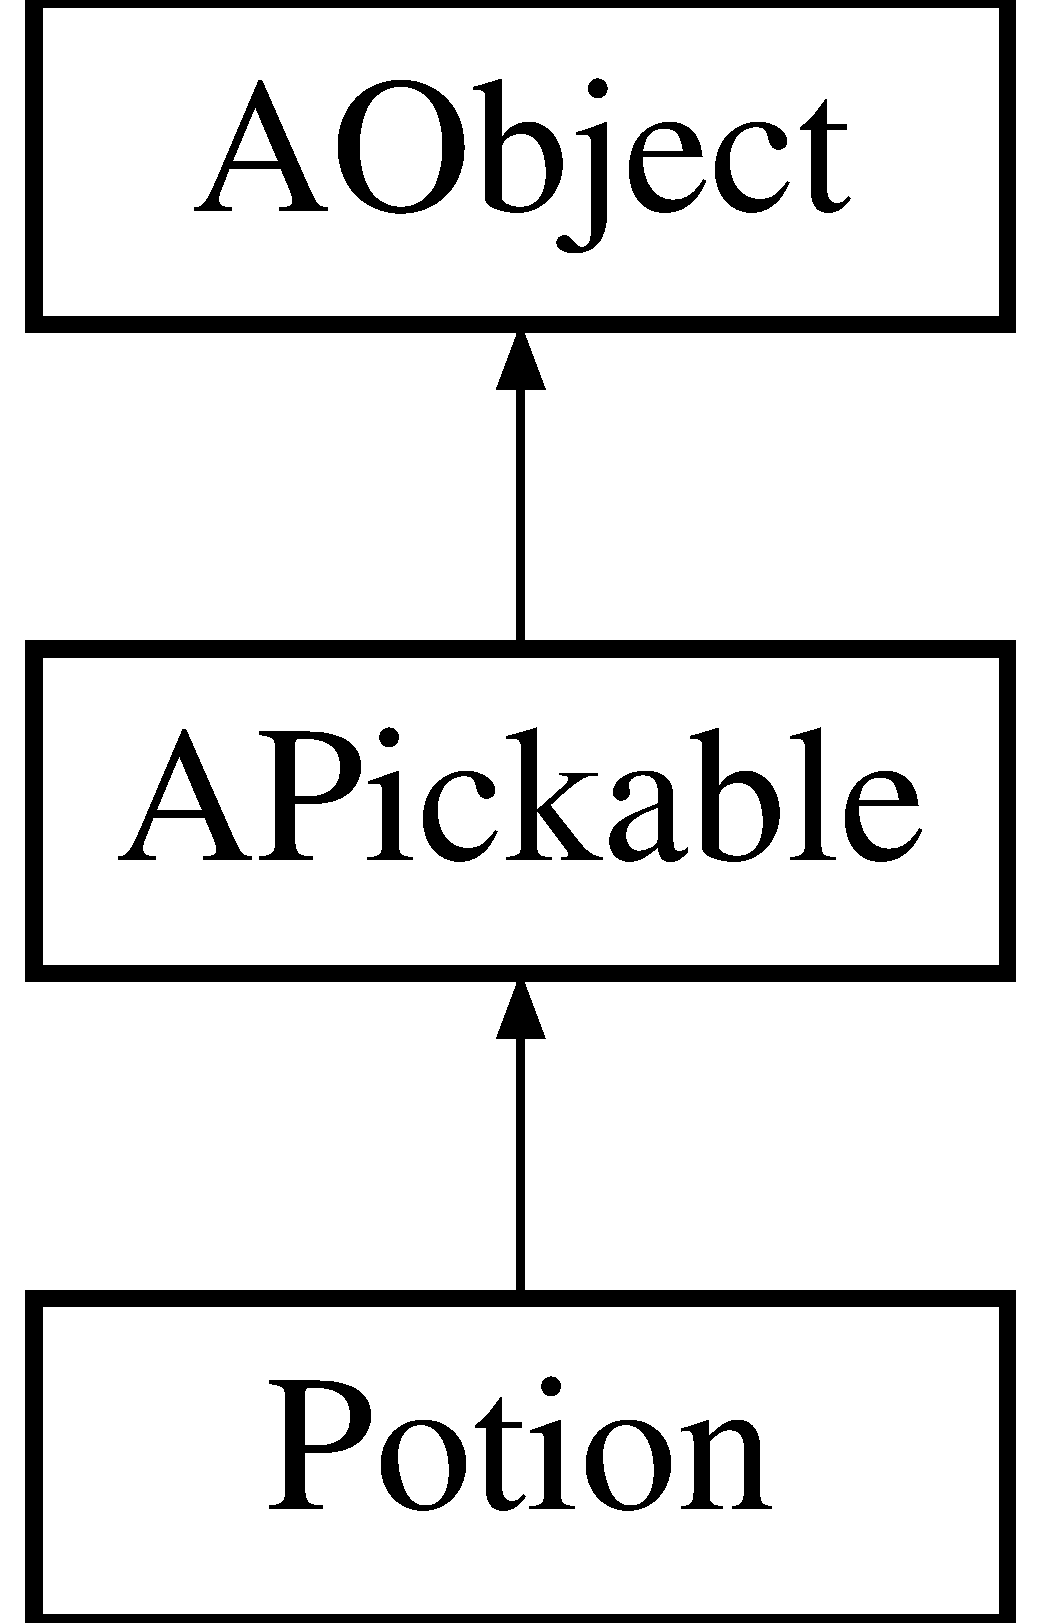
\includegraphics[height=3.000000cm]{classAObject}
\end{center}
\end{figure}
\subsection*{Public Member Functions}
\begin{DoxyCompactItemize}
\item 
\mbox{\Hypertarget{classAObject_a12a7789fca6342e9ff5c52c7cfd465d1}\label{classAObject_a12a7789fca6342e9ff5c52c7cfd465d1}} 
\hyperlink{classAObject_a12a7789fca6342e9ff5c52c7cfd465d1}{A\+Object} (std\+::shared\+\_\+ptr$<$ \hyperlink{classModel3d}{Model3d} $>$, indie\+::object\+Type=indie\+::object\+Type\+::\+U\+N\+K\+N\+OW, irr\+::u32 id=0)
\begin{DoxyCompactList}\small\item\em Constructor Build the class first param is a shared\+\_\+ptr on a \hyperlink{classModel3d}{Model3d}, second the type of object (C\+H\+E\+ST, P\+O\+T\+I\+ON, ...), third his id. \end{DoxyCompactList}\item 
\hyperlink{classAObject_ac17f3a1944792c280a3cbd83d839bc4e}{$\sim$\+A\+Object} ()
\begin{DoxyCompactList}\small\item\em Destructor. \end{DoxyCompactList}\item 
indie\+::object\+Type \hyperlink{classAObject_afcbaa047c0d02ca29b76875157a1eb1e}{get\+Type} () const
\begin{DoxyCompactList}\small\item\em get\+Type \end{DoxyCompactList}\item 
std\+::shared\+\_\+ptr$<$ \hyperlink{classModel3d}{Model3d} $>$ \hyperlink{classAObject_a3ffaa331c1842c5bf782c9a0343474bc}{get\+Model} () const
\begin{DoxyCompactList}\small\item\em get\+Model \end{DoxyCompactList}\item 
void \hyperlink{classAObject_ab4a2dc3dad1a54ff80d59c42a51479fb}{set\+Position} (Vector3d)
\begin{DoxyCompactList}\small\item\em set\+Position \end{DoxyCompactList}\item 
void \hyperlink{classAObject_a38ba628dcec6be910ce9d3c9f0de0de7}{set\+Rotation} (Vector3d)
\begin{DoxyCompactList}\small\item\em set\+Rotation \end{DoxyCompactList}\item 
void \hyperlink{classAObject_aebbd61ad13e23fa7787a5cdf12acd4ca}{print} () const
\begin{DoxyCompactList}\small\item\em print \end{DoxyCompactList}\item 
irr\+::u32 \hyperlink{classAObject_aae823d79b9bfa1ef090ee9e7b764de4a}{get\+Id} () const
\begin{DoxyCompactList}\small\item\em get\+Id \end{DoxyCompactList}\end{DoxyCompactItemize}


\subsection{Detailed Description}
An \hyperlink{classAObject}{A\+Object} instance has his own \hyperlink{classModel3d}{Model3d} attribute, and can modify it.. 

\subsection{Constructor \& Destructor Documentation}
\mbox{\Hypertarget{classAObject_ac17f3a1944792c280a3cbd83d839bc4e}\label{classAObject_ac17f3a1944792c280a3cbd83d839bc4e}} 
\index{A\+Object@{A\+Object}!````~A\+Object@{$\sim$\+A\+Object}}
\index{````~A\+Object@{$\sim$\+A\+Object}!A\+Object@{A\+Object}}
\subsubsection{\texorpdfstring{$\sim$\+A\+Object()}{~AObject()}}
{\footnotesize\ttfamily A\+Object\+::$\sim$\+A\+Object (\begin{DoxyParamCaption}{ }\end{DoxyParamCaption})}



Destructor. 

Destroy the class 

\subsection{Member Function Documentation}
\mbox{\Hypertarget{classAObject_aae823d79b9bfa1ef090ee9e7b764de4a}\label{classAObject_aae823d79b9bfa1ef090ee9e7b764de4a}} 
\index{A\+Object@{A\+Object}!get\+Id@{get\+Id}}
\index{get\+Id@{get\+Id}!A\+Object@{A\+Object}}
\subsubsection{\texorpdfstring{get\+Id()}{getId()}}
{\footnotesize\ttfamily irr\+::u32 A\+Object\+::get\+Id (\begin{DoxyParamCaption}{ }\end{DoxyParamCaption}) const}



get\+Id 

return the id of the \hyperlink{classAObject}{A\+Object} \mbox{\Hypertarget{classAObject_a3ffaa331c1842c5bf782c9a0343474bc}\label{classAObject_a3ffaa331c1842c5bf782c9a0343474bc}} 
\index{A\+Object@{A\+Object}!get\+Model@{get\+Model}}
\index{get\+Model@{get\+Model}!A\+Object@{A\+Object}}
\subsubsection{\texorpdfstring{get\+Model()}{getModel()}}
{\footnotesize\ttfamily std\+::shared\+\_\+ptr$<$ \hyperlink{classModel3d}{Model3d} $>$ A\+Object\+::get\+Model (\begin{DoxyParamCaption}{ }\end{DoxyParamCaption}) const}



get\+Model 

return the \hyperlink{classModel3d}{Model3d} of the \hyperlink{classAObject}{A\+Object} \mbox{\Hypertarget{classAObject_afcbaa047c0d02ca29b76875157a1eb1e}\label{classAObject_afcbaa047c0d02ca29b76875157a1eb1e}} 
\index{A\+Object@{A\+Object}!get\+Type@{get\+Type}}
\index{get\+Type@{get\+Type}!A\+Object@{A\+Object}}
\subsubsection{\texorpdfstring{get\+Type()}{getType()}}
{\footnotesize\ttfamily indie\+::object\+Type A\+Object\+::get\+Type (\begin{DoxyParamCaption}{ }\end{DoxyParamCaption}) const}



get\+Type 

return the type of the \hyperlink{classAObject}{A\+Object} \mbox{\Hypertarget{classAObject_aebbd61ad13e23fa7787a5cdf12acd4ca}\label{classAObject_aebbd61ad13e23fa7787a5cdf12acd4ca}} 
\index{A\+Object@{A\+Object}!print@{print}}
\index{print@{print}!A\+Object@{A\+Object}}
\subsubsection{\texorpdfstring{print()}{print()}}
{\footnotesize\ttfamily void A\+Object\+::print (\begin{DoxyParamCaption}{ }\end{DoxyParamCaption}) const}



print 

print the object on window \mbox{\Hypertarget{classAObject_ab4a2dc3dad1a54ff80d59c42a51479fb}\label{classAObject_ab4a2dc3dad1a54ff80d59c42a51479fb}} 
\index{A\+Object@{A\+Object}!set\+Position@{set\+Position}}
\index{set\+Position@{set\+Position}!A\+Object@{A\+Object}}
\subsubsection{\texorpdfstring{set\+Position()}{setPosition()}}
{\footnotesize\ttfamily void A\+Object\+::set\+Position (\begin{DoxyParamCaption}\item[{Vector3d}]{pos }\end{DoxyParamCaption})}



set\+Position 

change the vector position of the \hyperlink{classModel3d}{Model3d} of the \hyperlink{classAObject}{A\+Object} \mbox{\Hypertarget{classAObject_a38ba628dcec6be910ce9d3c9f0de0de7}\label{classAObject_a38ba628dcec6be910ce9d3c9f0de0de7}} 
\index{A\+Object@{A\+Object}!set\+Rotation@{set\+Rotation}}
\index{set\+Rotation@{set\+Rotation}!A\+Object@{A\+Object}}
\subsubsection{\texorpdfstring{set\+Rotation()}{setRotation()}}
{\footnotesize\ttfamily void A\+Object\+::set\+Rotation (\begin{DoxyParamCaption}\item[{Vector3d}]{rot }\end{DoxyParamCaption})}



set\+Rotation 

change the vector rotation of the \hyperlink{classModel3d}{Model3d} of the \hyperlink{classAObject}{A\+Object} 

The documentation for this class was generated from the following files\+:\begin{DoxyCompactItemize}
\item 
inc/game/character/heros/object/\hyperlink{AObject_8hh}{A\+Object.\+hh}\item 
src/game/character/heros/object/A\+Object.\+cpp\end{DoxyCompactItemize}

\hypertarget{classAPickable}{}\section{A\+Pickable Class Reference}
\label{classAPickable}\index{A\+Pickable@{A\+Pickable}}


create a pickable \hyperlink{classAObject}{A\+Object}  




{\ttfamily \#include $<$A\+Pickable.\+hh$>$}

Inheritance diagram for A\+Pickable\+:\begin{figure}[H]
\begin{center}
\leavevmode
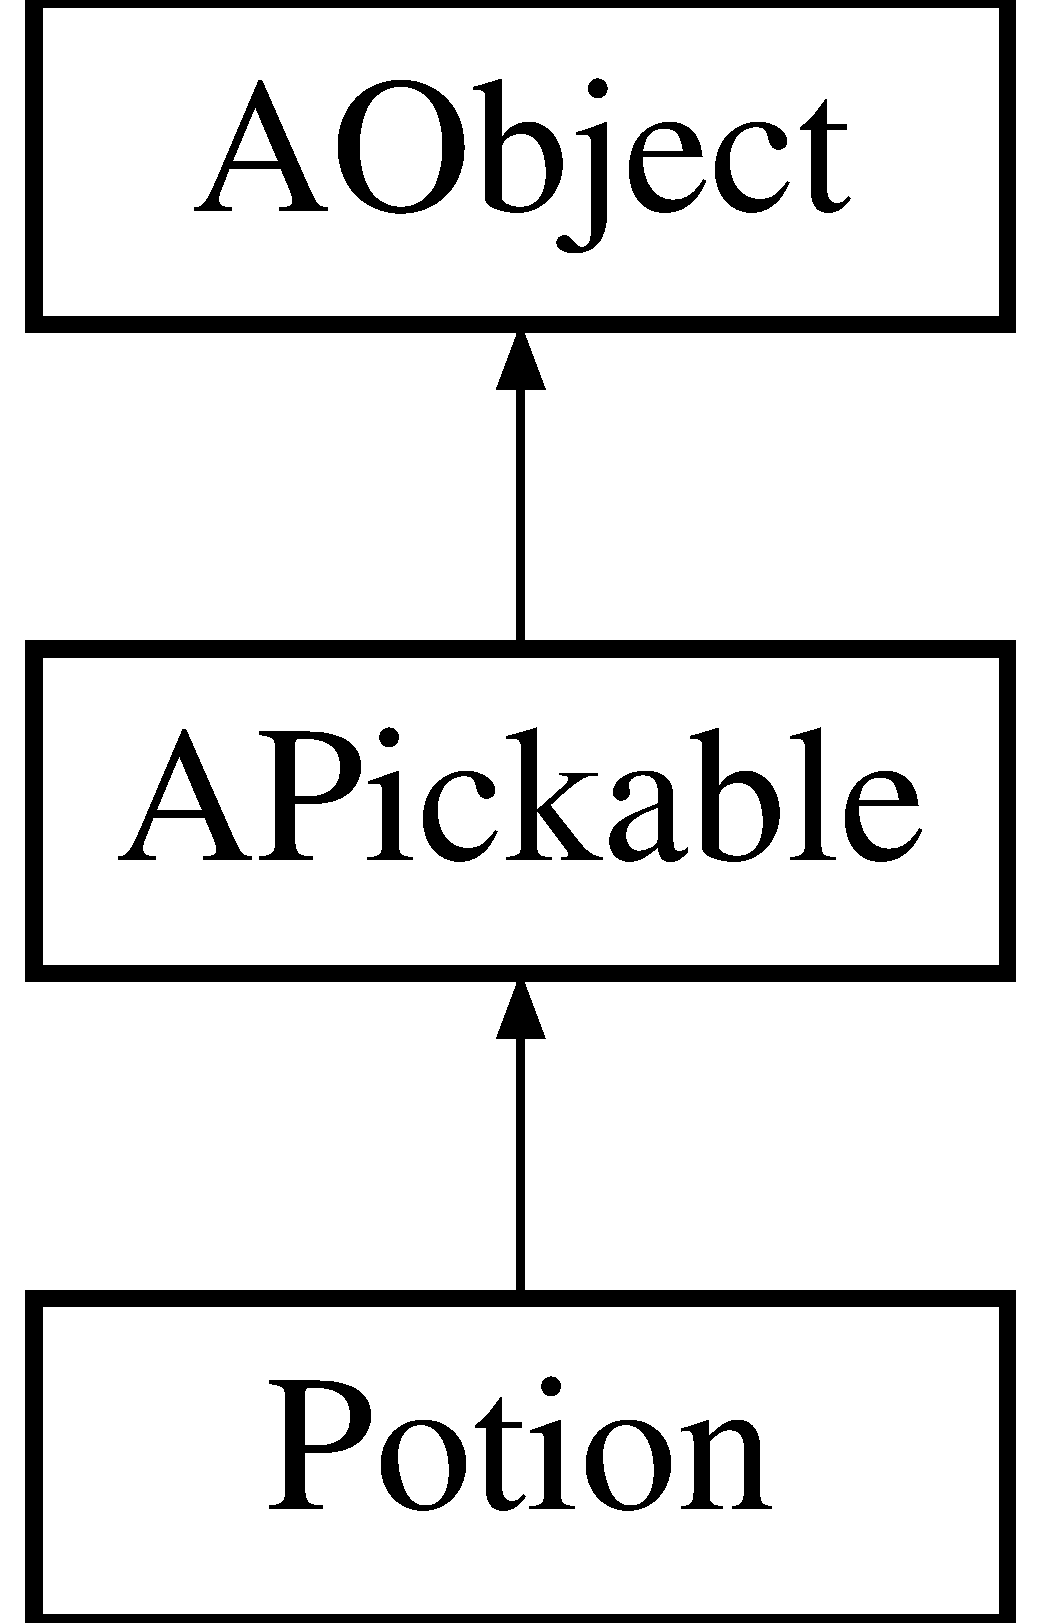
\includegraphics[height=3.000000cm]{classAPickable}
\end{center}
\end{figure}
\subsection*{Public Member Functions}
\begin{DoxyCompactItemize}
\item 
\hyperlink{classAPickable_a6be5419f2699d070f6e41c29deca6272}{A\+Pickable} (indie\+::object\+Type type)
\begin{DoxyCompactList}\small\item\em Constructor. \end{DoxyCompactList}\item 
\hyperlink{classAPickable_a145013963070158596ad2e0d07065f5d}{$\sim$\+A\+Pickable} ()
\begin{DoxyCompactList}\small\item\em Destructor. \end{DoxyCompactList}\end{DoxyCompactItemize}


\subsection{Detailed Description}
create a pickable \hyperlink{classAObject}{A\+Object} 

\subsection{Constructor \& Destructor Documentation}
\mbox{\Hypertarget{classAPickable_a6be5419f2699d070f6e41c29deca6272}\label{classAPickable_a6be5419f2699d070f6e41c29deca6272}} 
\index{A\+Pickable@{A\+Pickable}!A\+Pickable@{A\+Pickable}}
\index{A\+Pickable@{A\+Pickable}!A\+Pickable@{A\+Pickable}}
\subsubsection{\texorpdfstring{A\+Pickable()}{APickable()}}
{\footnotesize\ttfamily A\+Pickable\+::\+A\+Pickable (\begin{DoxyParamCaption}\item[{indie\+::object\+Type}]{type }\end{DoxyParamCaption})}



Constructor. 

Build the class \mbox{\Hypertarget{classAPickable_a145013963070158596ad2e0d07065f5d}\label{classAPickable_a145013963070158596ad2e0d07065f5d}} 
\index{A\+Pickable@{A\+Pickable}!````~A\+Pickable@{$\sim$\+A\+Pickable}}
\index{````~A\+Pickable@{$\sim$\+A\+Pickable}!A\+Pickable@{A\+Pickable}}
\subsubsection{\texorpdfstring{$\sim$\+A\+Pickable()}{~APickable()}}
{\footnotesize\ttfamily A\+Pickable\+::$\sim$\+A\+Pickable (\begin{DoxyParamCaption}{ }\end{DoxyParamCaption})}



Destructor. 

Destroy the class 

The documentation for this class was generated from the following files\+:\begin{DoxyCompactItemize}
\item 
inc/game/character/heros/object/\hyperlink{APickable_8hh}{A\+Pickable.\+hh}\item 
src/game/character/heros/object/A\+Pickable.\+cpp\end{DoxyCompactItemize}

\hypertarget{classAScene}{}\section{A\+Scene Class Reference}
\label{classAScene}\index{A\+Scene@{A\+Scene}}


Represent the window\textquotesingle{}s scene that will print some widget/object of the scene \+: buttons, images, etc...  




{\ttfamily \#include $<$A\+Scene.\+hh$>$}



Inherited by Credit\+Scene, Game\+Load\+Scene, Game\+Menu\+Scene, Game\+New\+Scene, Game\+Online\+Scene, Game\+Scene, Game\+Simulation\+Scene, Intro\+Scene, Legend\+Scene, Main\+Scene, Option\+Control\+Scene, Option\+Scene, Option\+Sound\+Scene, Option\+Video\+Scene, and Score\+Scene.

\subsection*{Public Member Functions}
\begin{DoxyCompactItemize}
\item 
\hyperlink{classAScene_ad0eacf691dbc8240fdf3a42d450c1042}{A\+Scene} ()
\begin{DoxyCompactList}\small\item\em Constructor. \end{DoxyCompactList}\item 
\hyperlink{classAScene_a9faf7f1a271327227e83627432d0b210}{$\sim$\+A\+Scene} ()
\begin{DoxyCompactList}\small\item\em Destructor. \end{DoxyCompactList}\item 
void \hyperlink{classAScene_ae5d7463a823ed64f3846b5847340b68c}{print} (\hyperlink{classWindow}{Window} $\ast$win)
\begin{DoxyCompactList}\small\item\em Print all the scene\textquotesingle{}s widgets into the \hyperlink{classWindow}{Window}. \end{DoxyCompactList}\item 
void \hyperlink{classAScene_a59f0acef6ed02a578062decd0f907773}{update} (\hyperlink{classWindow}{Window} $\ast$win)
\begin{DoxyCompactList}\small\item\em Update the Irrlicht tree, currently print into the window. \end{DoxyCompactList}\item 
void \hyperlink{classAScene_aa711b6068dd8dee262160eedfd96ad02}{add\+Widget} (const std\+::shared\+\_\+ptr$<$ \hyperlink{classIWidget}{I\+Widget} $>$ \&widget, Int id=-\/1)
\begin{DoxyCompactList}\small\item\em Allow the user to add texts, images, buttons, checkboxs or 3d models into the scene. \end{DoxyCompactList}\item 
void \hyperlink{classAScene_ad2b0ac8cd74a8523c76b681a34b5f5b4}{del\+Widget} (Int id)
\begin{DoxyCompactList}\small\item\em Allow the user to delete texts, images, buttons, checkboxs or 3d models into the scene. \end{DoxyCompactList}\item 
virtual irr\+::\+I\+Event\+Receiver $\ast$ \hyperlink{classAScene_af521e5e6d30a5d2e5d30eb333e4d3abd}{get\+Event\+Receiver} () const =0
\begin{DoxyCompactList}\small\item\em Allow the user to implemente the event callback class for each scene. \end{DoxyCompactList}\end{DoxyCompactItemize}


\subsection{Detailed Description}
Represent the window\textquotesingle{}s scene that will print some widget/object of the scene \+: buttons, images, etc... 

\subsection{Constructor \& Destructor Documentation}
\mbox{\Hypertarget{classAScene_ad0eacf691dbc8240fdf3a42d450c1042}\label{classAScene_ad0eacf691dbc8240fdf3a42d450c1042}} 
\index{A\+Scene@{A\+Scene}!A\+Scene@{A\+Scene}}
\index{A\+Scene@{A\+Scene}!A\+Scene@{A\+Scene}}
\subsubsection{\texorpdfstring{A\+Scene()}{AScene()}}
{\footnotesize\ttfamily A\+Scene\+::\+A\+Scene (\begin{DoxyParamCaption}{ }\end{DoxyParamCaption})}



Constructor. 

Build the class.


\begin{DoxyParams}{Parameters}
{\em None} & \\
\hline
\end{DoxyParams}
\mbox{\Hypertarget{classAScene_a9faf7f1a271327227e83627432d0b210}\label{classAScene_a9faf7f1a271327227e83627432d0b210}} 
\index{A\+Scene@{A\+Scene}!````~A\+Scene@{$\sim$\+A\+Scene}}
\index{````~A\+Scene@{$\sim$\+A\+Scene}!A\+Scene@{A\+Scene}}
\subsubsection{\texorpdfstring{$\sim$\+A\+Scene()}{~AScene()}}
{\footnotesize\ttfamily A\+Scene\+::$\sim$\+A\+Scene (\begin{DoxyParamCaption}{ }\end{DoxyParamCaption})}



Destructor. 

Destroy the class. 

\subsection{Member Function Documentation}
\mbox{\Hypertarget{classAScene_aa711b6068dd8dee262160eedfd96ad02}\label{classAScene_aa711b6068dd8dee262160eedfd96ad02}} 
\index{A\+Scene@{A\+Scene}!add\+Widget@{add\+Widget}}
\index{add\+Widget@{add\+Widget}!A\+Scene@{A\+Scene}}
\subsubsection{\texorpdfstring{add\+Widget()}{addWidget()}}
{\footnotesize\ttfamily void A\+Scene\+::add\+Widget (\begin{DoxyParamCaption}\item[{const std\+::shared\+\_\+ptr$<$ \hyperlink{classIWidget}{I\+Widget} $>$ \&}]{widget,  }\item[{Int}]{id = {\ttfamily -\/1} }\end{DoxyParamCaption})}



Allow the user to add texts, images, buttons, checkboxs or 3d models into the scene. 


\begin{DoxyParams}{Parameters}
{\em \textquotesingle{}widget\textquotesingle{}} & the widget to add in the scene. \\
\hline
\end{DoxyParams}
\mbox{\Hypertarget{classAScene_ad2b0ac8cd74a8523c76b681a34b5f5b4}\label{classAScene_ad2b0ac8cd74a8523c76b681a34b5f5b4}} 
\index{A\+Scene@{A\+Scene}!del\+Widget@{del\+Widget}}
\index{del\+Widget@{del\+Widget}!A\+Scene@{A\+Scene}}
\subsubsection{\texorpdfstring{del\+Widget()}{delWidget()}}
{\footnotesize\ttfamily void A\+Scene\+::del\+Widget (\begin{DoxyParamCaption}\item[{Int}]{id }\end{DoxyParamCaption})}



Allow the user to delete texts, images, buttons, checkboxs or 3d models into the scene. 

Example\+: scene-\/$>$add\+Widget(widget, 2); scene-\/$>$del\+Widget(2);


\begin{DoxyParams}{Parameters}
{\em \textquotesingle{}id\textquotesingle{}} & the widget\textquotesingle{}s id to del in the scene. \\
\hline
\end{DoxyParams}
\mbox{\Hypertarget{classAScene_af521e5e6d30a5d2e5d30eb333e4d3abd}\label{classAScene_af521e5e6d30a5d2e5d30eb333e4d3abd}} 
\index{A\+Scene@{A\+Scene}!get\+Event\+Receiver@{get\+Event\+Receiver}}
\index{get\+Event\+Receiver@{get\+Event\+Receiver}!A\+Scene@{A\+Scene}}
\subsubsection{\texorpdfstring{get\+Event\+Receiver()}{getEventReceiver()}}
{\footnotesize\ttfamily virtual irr\+::\+I\+Event\+Receiver$\ast$ A\+Scene\+::get\+Event\+Receiver (\begin{DoxyParamCaption}{ }\end{DoxyParamCaption}) const\hspace{0.3cm}{\ttfamily [pure virtual]}}



Allow the user to implemente the event callback class for each scene. 


\begin{DoxyParams}{Parameters}
{\em None.} & \\
\hline
\end{DoxyParams}
\begin{DoxyReturn}{Returns}
The events\textquotesingle{} receiver of the scene. 
\end{DoxyReturn}
\mbox{\Hypertarget{classAScene_ae5d7463a823ed64f3846b5847340b68c}\label{classAScene_ae5d7463a823ed64f3846b5847340b68c}} 
\index{A\+Scene@{A\+Scene}!print@{print}}
\index{print@{print}!A\+Scene@{A\+Scene}}
\subsubsection{\texorpdfstring{print()}{print()}}
{\footnotesize\ttfamily void A\+Scene\+::print (\begin{DoxyParamCaption}\item[{\hyperlink{classWindow}{Window} $\ast$}]{win }\end{DoxyParamCaption})}



Print all the scene\textquotesingle{}s widgets into the \hyperlink{classWindow}{Window}. 


\begin{DoxyParams}{Parameters}
{\em \textquotesingle{}win\textquotesingle{}} & the window where the scene will be print. \\
\hline
\end{DoxyParams}
\mbox{\Hypertarget{classAScene_a59f0acef6ed02a578062decd0f907773}\label{classAScene_a59f0acef6ed02a578062decd0f907773}} 
\index{A\+Scene@{A\+Scene}!update@{update}}
\index{update@{update}!A\+Scene@{A\+Scene}}
\subsubsection{\texorpdfstring{update()}{update()}}
{\footnotesize\ttfamily void A\+Scene\+::update (\begin{DoxyParamCaption}\item[{\hyperlink{classWindow}{Window} $\ast$}]{win }\end{DoxyParamCaption})}



Update the Irrlicht tree, currently print into the window. 


\begin{DoxyParams}{Parameters}
{\em \textquotesingle{}win\textquotesingle{}} & the window where the scene will be update. \\
\hline
\end{DoxyParams}


The documentation for this class was generated from the following files\+:\begin{DoxyCompactItemize}
\item 
inc/graphics/\hyperlink{AScene_8hh}{A\+Scene.\+hh}\item 
src/graphics/A\+Scene.\+cpp\end{DoxyCompactItemize}

\hypertarget{classButton}{}\section{Button Class Reference}
\label{classButton}\index{Button@{Button}}


Represent a button in the user interface.  




{\ttfamily \#include $<$Button.\+hh$>$}

Inheritance diagram for Button\+:\begin{figure}[H]
\begin{center}
\leavevmode
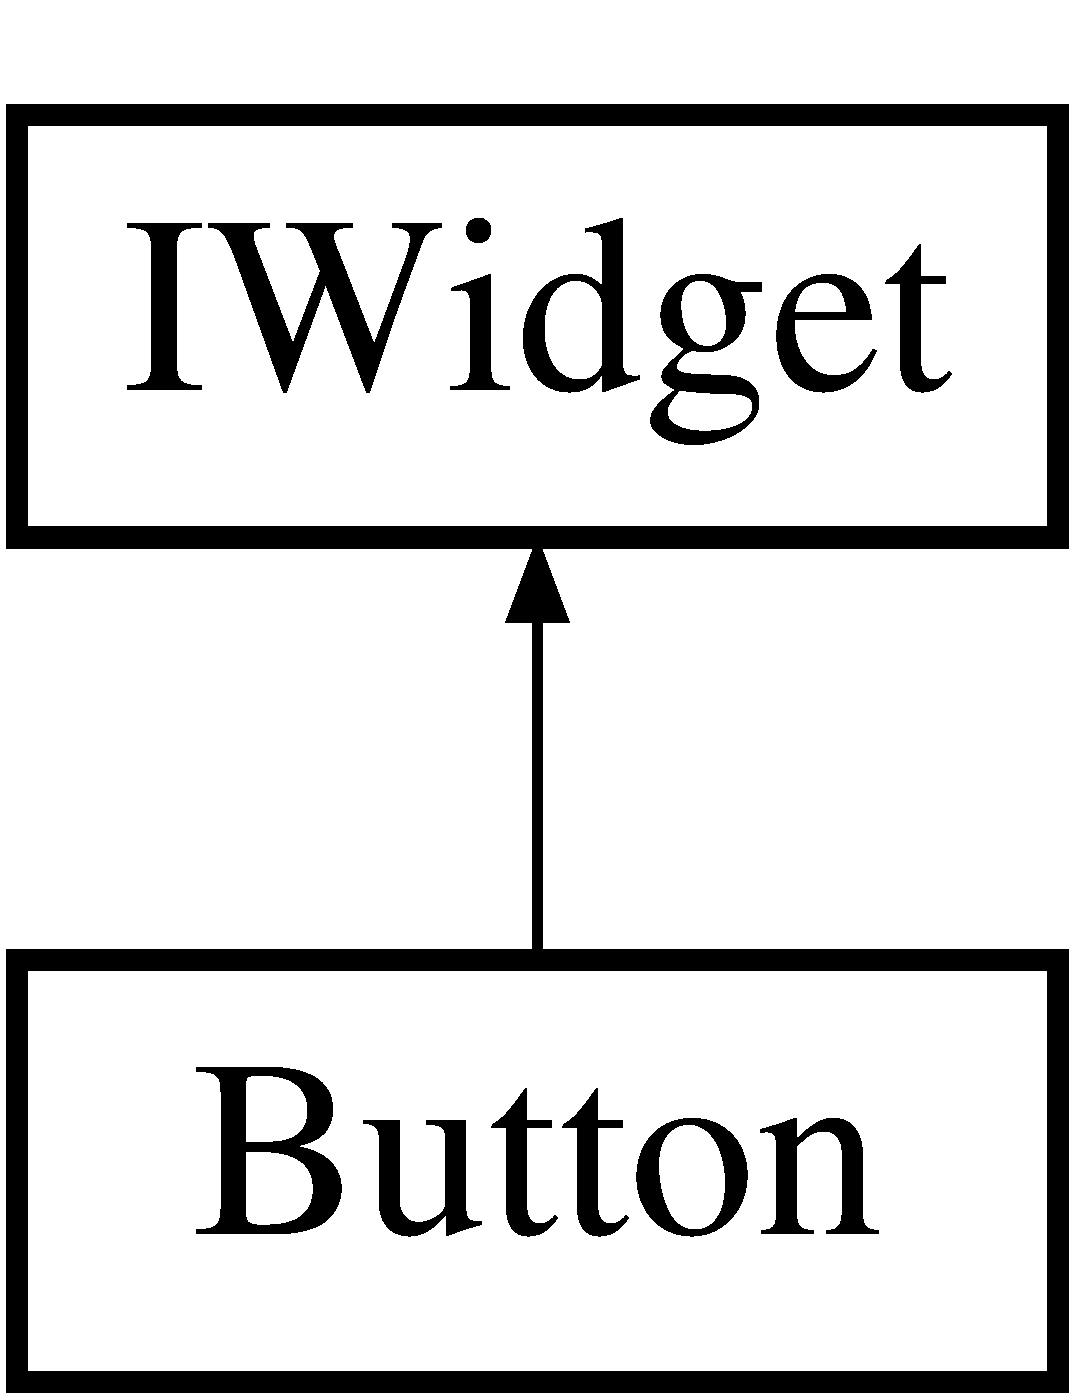
\includegraphics[height=2.000000cm]{classButton}
\end{center}
\end{figure}
\subsection*{Public Member Functions}
\begin{DoxyCompactItemize}
\item 
\hyperlink{classButton_a5729094ff8ec4ce3e64e6691c297983c}{Button} (const Rect \&rect, const wchar\+\_\+t $\ast$text, const wchar\+\_\+t $\ast$tooltext, enum indie\+::\+G\+U\+I\+Button\+Id id, const wchar\+\_\+t $\ast$background=L\char`\"{}assets/menus/transparent.\+png\char`\"{})
\begin{DoxyCompactList}\small\item\em Constructor. \end{DoxyCompactList}\item 
\mbox{\Hypertarget{classButton_a2a001eb9c3cc8ae54768a850dd345002}\label{classButton_a2a001eb9c3cc8ae54768a850dd345002}} 
\hyperlink{classButton_a2a001eb9c3cc8ae54768a850dd345002}{$\sim$\+Button} ()
\begin{DoxyCompactList}\small\item\em Destructor. \end{DoxyCompactList}\item 
void \hyperlink{classButton_aaee0c62414711ae91084b05b38d0c8c5}{print} (\hyperlink{classWindow}{Window} $\ast$win)
\begin{DoxyCompactList}\small\item\em Print the button into the window. \end{DoxyCompactList}\end{DoxyCompactItemize}


\subsection{Detailed Description}
Represent a button in the user interface. 

\subsection{Constructor \& Destructor Documentation}
\mbox{\Hypertarget{classButton_a5729094ff8ec4ce3e64e6691c297983c}\label{classButton_a5729094ff8ec4ce3e64e6691c297983c}} 
\index{Button@{Button}!Button@{Button}}
\index{Button@{Button}!Button@{Button}}
\subsubsection{\texorpdfstring{Button()}{Button()}}
{\footnotesize\ttfamily Button\+::\+Button (\begin{DoxyParamCaption}\item[{const Rect \&}]{rect,  }\item[{const wchar\+\_\+t $\ast$}]{text,  }\item[{const wchar\+\_\+t $\ast$}]{tooltext,  }\item[{enum indie\+::\+G\+U\+I\+Button\+Id}]{id,  }\item[{const wchar\+\_\+t $\ast$}]{background = {\ttfamily L\char`\"{}assets/menus/transparent.png\char`\"{}} }\end{DoxyParamCaption})}



Constructor. 

Build the class.


\begin{DoxyParams}{Parameters}
{\em rect} & The rectangle who represent the button (x1, y1, x2, y2). \\
\hline
{\em background} & The name of the image, that will be put on the background of the button. \\
\hline
{\em text} & the text that will be write on the button. \\
\hline
{\em tooltext} & The text displayed in the tooltip. \\
\hline
{\em id} & The id throw the user click on the button . \\
\hline
\end{DoxyParams}


\subsection{Member Function Documentation}
\mbox{\Hypertarget{classButton_aaee0c62414711ae91084b05b38d0c8c5}\label{classButton_aaee0c62414711ae91084b05b38d0c8c5}} 
\index{Button@{Button}!print@{print}}
\index{print@{print}!Button@{Button}}
\subsubsection{\texorpdfstring{print()}{print()}}
{\footnotesize\ttfamily void Button\+::print (\begin{DoxyParamCaption}\item[{\hyperlink{classWindow}{Window} $\ast$}]{win }\end{DoxyParamCaption})\hspace{0.3cm}{\ttfamily [virtual]}}



Print the button into the window. 


\begin{DoxyParams}{Parameters}
{\em win} & The window where the button will be print. \\
\hline
\end{DoxyParams}


Implements \hyperlink{classIWidget_a0cfa49a402e9bb31808a715e048ab2f4}{I\+Widget}.



The documentation for this class was generated from the following files\+:\begin{DoxyCompactItemize}
\item 
inc/graphics/widgets/\hyperlink{Button_8hh}{Button.\+hh}\item 
src/graphics/widgets/Button.\+cpp\end{DoxyCompactItemize}

\hypertarget{classCamera}{}\section{Camera Class Reference}
\label{classCamera}\index{Camera@{Camera}}


where cameras behaviour is defined  




{\ttfamily \#include $<$Camera.\+hh$>$}

\subsection*{Public Member Functions}
\begin{DoxyCompactItemize}
\item 
\hyperlink{classCamera_a4ffc956956f49716d7fa3bff2591cd3a}{Camera} (\hyperlink{classirr_1_1scene_1_1ICameraSceneNode}{irr\+::scene\+::\+I\+Camera\+Scene\+Node} $\ast$const cam)
\begin{DoxyCompactList}\small\item\em instanciate \hyperlink{classCamera}{Camera} \end{DoxyCompactList}\item 
\mbox{\Hypertarget{classCamera_ad1897942d0ccf91052386388a497349f}\label{classCamera_ad1897942d0ccf91052386388a497349f}} 
\hyperlink{classCamera_ad1897942d0ccf91052386388a497349f}{$\sim$\+Camera} ()
\begin{DoxyCompactList}\small\item\em Destructor... \end{DoxyCompactList}\item 
void \hyperlink{classCamera_ad7d58a7f1ab2b31f120a0bdad677b300}{change\+Position} (\hyperlink{namespaceirr_1_1core_a06f169d08b5c429f5575acb7edbad811}{irr\+::core\+::vector3df} move)
\begin{DoxyCompactList}\small\item\em change absolute camera position \end{DoxyCompactList}\item 
void \hyperlink{classCamera_a8c11f289be05671191a4f91288155685}{change\+Sight} (\hyperlink{namespaceirr_1_1core_a06f169d08b5c429f5575acb7edbad811}{irr\+::core\+::vector3df} new\+Target)
\begin{DoxyCompactList}\small\item\em change camera sight \end{DoxyCompactList}\end{DoxyCompactItemize}


\subsection{Detailed Description}
where cameras behaviour is defined 

\subsection{Constructor \& Destructor Documentation}
\mbox{\Hypertarget{classCamera_a4ffc956956f49716d7fa3bff2591cd3a}\label{classCamera_a4ffc956956f49716d7fa3bff2591cd3a}} 
\index{Camera@{Camera}!Camera@{Camera}}
\index{Camera@{Camera}!Camera@{Camera}}
\subsubsection{\texorpdfstring{Camera()}{Camera()}}
{\footnotesize\ttfamily Camera\+::\+Camera (\begin{DoxyParamCaption}\item[{\hyperlink{classirr_1_1scene_1_1ICameraSceneNode}{irr\+::scene\+::\+I\+Camera\+Scene\+Node} $\ast$const}]{cam }\end{DoxyParamCaption})}



instanciate \hyperlink{classCamera}{Camera} 


\begin{DoxyParams}{Parameters}
{\em cam} & \+: the irrlicht static camera \\
\hline
\end{DoxyParams}


\subsection{Member Function Documentation}
\mbox{\Hypertarget{classCamera_ad7d58a7f1ab2b31f120a0bdad677b300}\label{classCamera_ad7d58a7f1ab2b31f120a0bdad677b300}} 
\index{Camera@{Camera}!change\+Position@{change\+Position}}
\index{change\+Position@{change\+Position}!Camera@{Camera}}
\subsubsection{\texorpdfstring{change\+Position()}{changePosition()}}
{\footnotesize\ttfamily void Camera\+::change\+Position (\begin{DoxyParamCaption}\item[{\hyperlink{namespaceirr_1_1core_a06f169d08b5c429f5575acb7edbad811}{irr\+::core\+::vector3df}}]{move }\end{DoxyParamCaption})}



change absolute camera position 


\begin{DoxyParams}{Parameters}
{\em move} & \+: irrlicht 3D vector to positions camera \\
\hline
\end{DoxyParams}
\mbox{\Hypertarget{classCamera_a8c11f289be05671191a4f91288155685}\label{classCamera_a8c11f289be05671191a4f91288155685}} 
\index{Camera@{Camera}!change\+Sight@{change\+Sight}}
\index{change\+Sight@{change\+Sight}!Camera@{Camera}}
\subsubsection{\texorpdfstring{change\+Sight()}{changeSight()}}
{\footnotesize\ttfamily void Camera\+::change\+Sight (\begin{DoxyParamCaption}\item[{\hyperlink{namespaceirr_1_1core_a06f169d08b5c429f5575acb7edbad811}{irr\+::core\+::vector3df}}]{new\+Target }\end{DoxyParamCaption})}



change camera sight 



The documentation for this class was generated from the following files\+:\begin{DoxyCompactItemize}
\item 
inc/graphics/\hyperlink{Camera_8hh}{Camera.\+hh}\item 
src/graphics/Camera.\+cpp\end{DoxyCompactItemize}

\hypertarget{classConfigManager}{}\section{Config\+Manager Class Reference}
\label{classConfigManager}\index{Config\+Manager@{Config\+Manager}}


This class contain all the methode to manipulate the configuration.  




{\ttfamily \#include $<$Config\+Manager.\+hh$>$}

\subsection*{Public Member Functions}
\begin{DoxyCompactItemize}
\item 
\hyperlink{classConfigManager_a7d3d7c10423d969f7544509f6fcca32f}{Config\+Manager} ()
\begin{DoxyCompactList}\small\item\em Constructor. \end{DoxyCompactList}\item 
void \hyperlink{classConfigManager_a63ff6c831f037cf5bfe580b4944b0b6c}{load\+Config} (std\+::string)
\begin{DoxyCompactList}\small\item\em Load the configuration. \end{DoxyCompactList}\item 
\mbox{\Hypertarget{classConfigManager_a178e051860792271e9b1ec4434776f91}\label{classConfigManager_a178e051860792271e9b1ec4434776f91}} 
void \hyperlink{classConfigManager_a178e051860792271e9b1ec4434776f91}{save\+Config} () const
\begin{DoxyCompactList}\small\item\em Savethe object in the file. \end{DoxyCompactList}\item 
void \hyperlink{classConfigManager_a4f2b06f2ef741a15b3dfe82259cfd355}{create\+File} (std\+::string)
\begin{DoxyCompactList}\small\item\em create an empty configuration file \end{DoxyCompactList}\end{DoxyCompactItemize}
\subsection*{Public Attributes}
\begin{DoxyCompactItemize}
\item 
config\+::\+Video \hyperlink{classConfigManager_a1e0dbb8563b71871e6c68abce5620cd0}{video\+Config}
\begin{DoxyCompactList}\small\item\em The object video\+Config is a structure that contain all the setting for the video. \end{DoxyCompactList}\item 
config\+::\+Sound \hyperlink{classConfigManager_a010e2da02ebc90d7ce930d1c57a79e96}{sound}
\begin{DoxyCompactList}\small\item\em The object sound is a structure that constain all the setting for the sound. \end{DoxyCompactList}\item 
\mbox{\Hypertarget{classConfigManager_ad6d6269ec9827af5ca12067a49383132}\label{classConfigManager_ad6d6269ec9827af5ca12067a49383132}} 
std\+::vector$<$ config\+::\+I\+Control $>$ \hyperlink{classConfigManager_ad6d6269ec9827af5ca12067a49383132}{controllers}
\begin{DoxyCompactList}\small\item\em The object controllers is a vector that contain all the configuration for each players. \end{DoxyCompactList}\end{DoxyCompactItemize}


\subsection{Detailed Description}
This class contain all the methode to manipulate the configuration. 

\subsection{Constructor \& Destructor Documentation}
\mbox{\Hypertarget{classConfigManager_a7d3d7c10423d969f7544509f6fcca32f}\label{classConfigManager_a7d3d7c10423d969f7544509f6fcca32f}} 
\index{Config\+Manager@{Config\+Manager}!Config\+Manager@{Config\+Manager}}
\index{Config\+Manager@{Config\+Manager}!Config\+Manager@{Config\+Manager}}
\subsubsection{\texorpdfstring{Config\+Manager()}{ConfigManager()}}
{\footnotesize\ttfamily Config\+Manager\+::\+Config\+Manager (\begin{DoxyParamCaption}{ }\end{DoxyParamCaption})}



Constructor. 

Build the class


\begin{DoxyParams}{Parameters}
{\em nothing} & \\
\hline
\end{DoxyParams}


\subsection{Member Function Documentation}
\mbox{\Hypertarget{classConfigManager_a4f2b06f2ef741a15b3dfe82259cfd355}\label{classConfigManager_a4f2b06f2ef741a15b3dfe82259cfd355}} 
\index{Config\+Manager@{Config\+Manager}!create\+File@{create\+File}}
\index{create\+File@{create\+File}!Config\+Manager@{Config\+Manager}}
\subsubsection{\texorpdfstring{create\+File()}{createFile()}}
{\footnotesize\ttfamily void Config\+Manager\+::create\+File (\begin{DoxyParamCaption}\item[{std\+::string}]{file\+Name }\end{DoxyParamCaption})}



create an empty configuration file 


\begin{DoxyParams}{Parameters}
{\em path} & to the new configuration file \\
\hline
\end{DoxyParams}
\mbox{\Hypertarget{classConfigManager_a63ff6c831f037cf5bfe580b4944b0b6c}\label{classConfigManager_a63ff6c831f037cf5bfe580b4944b0b6c}} 
\index{Config\+Manager@{Config\+Manager}!load\+Config@{load\+Config}}
\index{load\+Config@{load\+Config}!Config\+Manager@{Config\+Manager}}
\subsubsection{\texorpdfstring{load\+Config()}{loadConfig()}}
{\footnotesize\ttfamily void Config\+Manager\+::load\+Config (\begin{DoxyParamCaption}\item[{std\+::string}]{file\+Name }\end{DoxyParamCaption})}



Load the configuration. 


\begin{DoxyParams}{Parameters}
{\em path} & to the configuration file \\
\hline
\end{DoxyParams}
\begin{DoxyReturn}{Returns}
void 
\end{DoxyReturn}


\subsection{Member Data Documentation}
\mbox{\Hypertarget{classConfigManager_a010e2da02ebc90d7ce930d1c57a79e96}\label{classConfigManager_a010e2da02ebc90d7ce930d1c57a79e96}} 
\index{Config\+Manager@{Config\+Manager}!sound@{sound}}
\index{sound@{sound}!Config\+Manager@{Config\+Manager}}
\subsubsection{\texorpdfstring{sound}{sound}}
{\footnotesize\ttfamily config\+::\+Sound Config\+Manager\+::sound}



The object sound is a structure that constain all the setting for the sound. 

The sructure is on the config namespace \mbox{\Hypertarget{classConfigManager_a1e0dbb8563b71871e6c68abce5620cd0}\label{classConfigManager_a1e0dbb8563b71871e6c68abce5620cd0}} 
\index{Config\+Manager@{Config\+Manager}!video\+Config@{video\+Config}}
\index{video\+Config@{video\+Config}!Config\+Manager@{Config\+Manager}}
\subsubsection{\texorpdfstring{video\+Config}{videoConfig}}
{\footnotesize\ttfamily config\+::\+Video Config\+Manager\+::video\+Config}



The object video\+Config is a structure that contain all the setting for the video. 

The sructure is on the config namespace 

The documentation for this class was generated from the following files\+:\begin{DoxyCompactItemize}
\item 
inc/managers/\hyperlink{ConfigManager_8hh}{Config\+Manager.\+hh}\item 
src/managers/Config\+Manager.\+cpp\end{DoxyCompactItemize}

\hypertarget{structconfig_1_1Control}{}\section{config\+:\+:Control Struct Reference}
\label{structconfig_1_1Control}\index{config\+::\+Control@{config\+::\+Control}}


This structure contain two \hyperlink{structconfig_1_1ControlPlayer}{Control\+Player} structure (one for each player)  




{\ttfamily \#include $<$Control.\+hh$>$}



\subsection{Detailed Description}
This structure contain two \hyperlink{structconfig_1_1ControlPlayer}{Control\+Player} structure (one for each player) 

The documentation for this struct was generated from the following file\+:\begin{DoxyCompactItemize}
\item 
inc/managers/config/\hyperlink{Control_8hh}{Control.\+hh}\end{DoxyCompactItemize}

\hypertarget{classController}{}\section{Controller Class Reference}
\label{classController}\index{Controller@{Controller}}


Use to handle \hyperlink{classController}{Controller} Event.  




{\ttfamily \#include $<$Controller.\+hh$>$}



Inherits I\+Event\+Receiver.

\subsection*{Public Member Functions}
\begin{DoxyCompactItemize}
\item 
\hyperlink{classController_ac4a14971762c0d091606211711762273}{Controller} (const irr\+::u32 controller\+ID, const irr\+::u32 player\+ID)
\begin{DoxyCompactList}\small\item\em Constructor. \end{DoxyCompactList}\item 
\hyperlink{classController_a0ab87934c4f7a266cfdb86e0f36bc1b5}{$\sim$\+Controller} ()
\begin{DoxyCompactList}\small\item\em Destructor. \end{DoxyCompactList}\item 
virtual bool \hyperlink{classController_a81b6f6d728022c92b064866759a7d4d9}{On\+Event} (const irr\+::\+S\+Event \&event)
\begin{DoxyCompactList}\small\item\em On\+Event. \end{DoxyCompactList}\item 
const irr\+::\+S\+Event\+::\+S\+Joystick\+Event \& \hyperlink{classController_a43d5202e40ae827029fdca587d0bfeab}{get\+Joystick\+State} (void) const
\begin{DoxyCompactList}\small\item\em get\+Joystick\+State \end{DoxyCompactList}\item 
irr\+::core\+::array$<$ irr\+::\+S\+Joystick\+Info $>$ \& \hyperlink{classController_a1d628add26120f35d2dc53eabaa34d4b}{get\+Joystick\+Info} (void)
\begin{DoxyCompactList}\small\item\em get\+Joystick\+Info \end{DoxyCompactList}\item 
void \hyperlink{classController_a3e855bf7e018e2659ecb3d0e13a7f39c}{notify\+Event\+Manager} (void)
\begin{DoxyCompactList}\small\item\em notify\+Event\+Manager \end{DoxyCompactList}\item 
irr\+::u32 \hyperlink{classController_a76891bd0871480c92f45c597c3eddf93}{get\+Player\+ID} (void) const
\begin{DoxyCompactList}\small\item\em get\+Player\+ID \end{DoxyCompactList}\item 
irr\+::u32 \hyperlink{classController_ab2294a9b730b80216705b7e9ae36a5bd}{get\+Controller\+ID} (void) const
\begin{DoxyCompactList}\small\item\em get\+Controller\+ID \end{DoxyCompactList}\end{DoxyCompactItemize}


\subsection{Detailed Description}
Use to handle \hyperlink{classController}{Controller} Event. 

\subsection{Constructor \& Destructor Documentation}
\mbox{\Hypertarget{classController_ac4a14971762c0d091606211711762273}\label{classController_ac4a14971762c0d091606211711762273}} 
\index{Controller@{Controller}!Controller@{Controller}}
\index{Controller@{Controller}!Controller@{Controller}}
\subsubsection{\texorpdfstring{Controller()}{Controller()}}
{\footnotesize\ttfamily Controller\+::\+Controller (\begin{DoxyParamCaption}\item[{const irr\+::u32}]{controller\+ID,  }\item[{const irr\+::u32}]{player\+ID }\end{DoxyParamCaption})}



Constructor. 

Build the class


\begin{DoxyParams}{Parameters}
{\em controller\+ID} & Define the id of controller\\
\hline
{\em player\+ID} & Define the id of player \\
\hline
\end{DoxyParams}
\mbox{\Hypertarget{classController_a0ab87934c4f7a266cfdb86e0f36bc1b5}\label{classController_a0ab87934c4f7a266cfdb86e0f36bc1b5}} 
\index{Controller@{Controller}!````~Controller@{$\sim$\+Controller}}
\index{````~Controller@{$\sim$\+Controller}!Controller@{Controller}}
\subsubsection{\texorpdfstring{$\sim$\+Controller()}{~Controller()}}
{\footnotesize\ttfamily Controller\+::$\sim$\+Controller (\begin{DoxyParamCaption}{ }\end{DoxyParamCaption})}



Destructor. 

Destruct the class 

\subsection{Member Function Documentation}
\mbox{\Hypertarget{classController_ab2294a9b730b80216705b7e9ae36a5bd}\label{classController_ab2294a9b730b80216705b7e9ae36a5bd}} 
\index{Controller@{Controller}!get\+Controller\+ID@{get\+Controller\+ID}}
\index{get\+Controller\+ID@{get\+Controller\+ID}!Controller@{Controller}}
\subsubsection{\texorpdfstring{get\+Controller\+I\+D()}{getControllerID()}}
{\footnotesize\ttfamily Unsigned\+Int Controller\+::get\+Controller\+ID (\begin{DoxyParamCaption}\item[{void}]{ }\end{DoxyParamCaption}) const}



get\+Controller\+ID 

\begin{DoxyReturn}{Returns}
\+\_\+controller\+ID 
\end{DoxyReturn}
\mbox{\Hypertarget{classController_a1d628add26120f35d2dc53eabaa34d4b}\label{classController_a1d628add26120f35d2dc53eabaa34d4b}} 
\index{Controller@{Controller}!get\+Joystick\+Info@{get\+Joystick\+Info}}
\index{get\+Joystick\+Info@{get\+Joystick\+Info}!Controller@{Controller}}
\subsubsection{\texorpdfstring{get\+Joystick\+Info()}{getJoystickInfo()}}
{\footnotesize\ttfamily irr\+::core\+::array$<$irr\+::\+S\+Joystick\+Info$>$\& Controller\+::get\+Joystick\+Info (\begin{DoxyParamCaption}\item[{void}]{ }\end{DoxyParamCaption})}



get\+Joystick\+Info 

\begin{DoxyReturn}{Returns}
the \+\_\+joystick\+Info 
\end{DoxyReturn}
\mbox{\Hypertarget{classController_a43d5202e40ae827029fdca587d0bfeab}\label{classController_a43d5202e40ae827029fdca587d0bfeab}} 
\index{Controller@{Controller}!get\+Joystick\+State@{get\+Joystick\+State}}
\index{get\+Joystick\+State@{get\+Joystick\+State}!Controller@{Controller}}
\subsubsection{\texorpdfstring{get\+Joystick\+State()}{getJoystickState()}}
{\footnotesize\ttfamily const irr\+::\+S\+Event\+::\+S\+Joystick\+Event\& Controller\+::get\+Joystick\+State (\begin{DoxyParamCaption}\item[{void}]{ }\end{DoxyParamCaption}) const}



get\+Joystick\+State 

\begin{DoxyReturn}{Returns}
the state of \+\_\+joystick\+State 
\end{DoxyReturn}
\mbox{\Hypertarget{classController_a76891bd0871480c92f45c597c3eddf93}\label{classController_a76891bd0871480c92f45c597c3eddf93}} 
\index{Controller@{Controller}!get\+Player\+ID@{get\+Player\+ID}}
\index{get\+Player\+ID@{get\+Player\+ID}!Controller@{Controller}}
\subsubsection{\texorpdfstring{get\+Player\+I\+D()}{getPlayerID()}}
{\footnotesize\ttfamily Unsigned\+Int Controller\+::get\+Player\+ID (\begin{DoxyParamCaption}\item[{void}]{ }\end{DoxyParamCaption}) const}



get\+Player\+ID 

\begin{DoxyReturn}{Returns}
\+\_\+player\+ID 
\end{DoxyReturn}
\mbox{\Hypertarget{classController_a3e855bf7e018e2659ecb3d0e13a7f39c}\label{classController_a3e855bf7e018e2659ecb3d0e13a7f39c}} 
\index{Controller@{Controller}!notify\+Event\+Manager@{notify\+Event\+Manager}}
\index{notify\+Event\+Manager@{notify\+Event\+Manager}!Controller@{Controller}}
\subsubsection{\texorpdfstring{notify\+Event\+Manager()}{notifyEventManager()}}
{\footnotesize\ttfamily void Controller\+::notify\+Event\+Manager (\begin{DoxyParamCaption}\item[{void}]{ }\end{DoxyParamCaption})}



notify\+Event\+Manager 

Add the event to the Event\+Manager queue \mbox{\Hypertarget{classController_a81b6f6d728022c92b064866759a7d4d9}\label{classController_a81b6f6d728022c92b064866759a7d4d9}} 
\index{Controller@{Controller}!On\+Event@{On\+Event}}
\index{On\+Event@{On\+Event}!Controller@{Controller}}
\subsubsection{\texorpdfstring{On\+Event()}{OnEvent()}}
{\footnotesize\ttfamily bool Controller\+::\+On\+Event (\begin{DoxyParamCaption}\item[{const irr\+::\+S\+Event \&}]{event }\end{DoxyParamCaption})\hspace{0.3cm}{\ttfamily [virtual]}}



On\+Event. 

Handle the event


\begin{DoxyParams}{Parameters}
{\em event} & Event sent by irrlicht \\
\hline
\end{DoxyParams}


The documentation for this class was generated from the following files\+:\begin{DoxyCompactItemize}
\item 
inc/event/\hyperlink{Controller_8hh}{Controller.\+hh}\item 
src/event/Controller.\+cpp\end{DoxyCompactItemize}

\hypertarget{classControlManager}{}\section{Control\+Manager Class Reference}
\label{classControlManager}\index{Control\+Manager@{Control\+Manager}}


Manage the \hyperlink{classController}{Controller} Instance.  




{\ttfamily \#include $<$Control\+Manager.\+hh$>$}

\subsection*{Public Member Functions}
\begin{DoxyCompactItemize}
\item 
\hyperlink{classControlManager_ac47df3d59d665fa9e6201677689ddf6a}{Control\+Manager} ()
\begin{DoxyCompactList}\small\item\em Contructor. \end{DoxyCompactList}\item 
\hyperlink{classControlManager_a58c547d9cb07dfaa0d6967cc656b80cb}{$\sim$\+Control\+Manager} ()
\begin{DoxyCompactList}\small\item\em Destructor. \end{DoxyCompactList}\end{DoxyCompactItemize}


\subsection{Detailed Description}
Manage the \hyperlink{classController}{Controller} Instance. 

\subsection{Constructor \& Destructor Documentation}
\mbox{\Hypertarget{classControlManager_ac47df3d59d665fa9e6201677689ddf6a}\label{classControlManager_ac47df3d59d665fa9e6201677689ddf6a}} 
\index{Control\+Manager@{Control\+Manager}!Control\+Manager@{Control\+Manager}}
\index{Control\+Manager@{Control\+Manager}!Control\+Manager@{Control\+Manager}}
\subsubsection{\texorpdfstring{Control\+Manager()}{ControlManager()}}
{\footnotesize\ttfamily Control\+Manager\+::\+Control\+Manager (\begin{DoxyParamCaption}{ }\end{DoxyParamCaption})}



Contructor. 

Build the class \mbox{\Hypertarget{classControlManager_a58c547d9cb07dfaa0d6967cc656b80cb}\label{classControlManager_a58c547d9cb07dfaa0d6967cc656b80cb}} 
\index{Control\+Manager@{Control\+Manager}!````~Control\+Manager@{$\sim$\+Control\+Manager}}
\index{````~Control\+Manager@{$\sim$\+Control\+Manager}!Control\+Manager@{Control\+Manager}}
\subsubsection{\texorpdfstring{$\sim$\+Control\+Manager()}{~ControlManager()}}
{\footnotesize\ttfamily Control\+Manager\+::$\sim$\+Control\+Manager (\begin{DoxyParamCaption}{ }\end{DoxyParamCaption})}



Destructor. 

Destroy the class 

The documentation for this class was generated from the following files\+:\begin{DoxyCompactItemize}
\item 
inc/managers/\hyperlink{ControlManager_8hh}{Control\+Manager.\+hh}\item 
src/managers/Control\+Manager.\+cpp\end{DoxyCompactItemize}

\hypertarget{structconfig_1_1ControlPlayer}{}\section{config\+:\+:Control\+Player Struct Reference}
\label{structconfig_1_1ControlPlayer}\index{config\+::\+Control\+Player@{config\+::\+Control\+Player}}


This structure contain all the key that are necessary to a player.  




{\ttfamily \#include $<$Control.\+hh$>$}



\subsection{Detailed Description}
This structure contain all the key that are necessary to a player. 

The documentation for this struct was generated from the following file\+:\begin{DoxyCompactItemize}
\item 
inc/managers/config/\hyperlink{Control_8hh}{Control.\+hh}\end{DoxyCompactItemize}

\hypertarget{classCoreManager}{}\section{Core\+Manager Class Reference}
\label{classCoreManager}\index{Core\+Manager@{Core\+Manager}}


\hyperlink{classCoreManager}{Core\+Manager} is the main manager who regroups all the other manager.  




{\ttfamily \#include $<$Core\+Manager.\+hh$>$}

\subsection*{Public Member Functions}
\begin{DoxyCompactItemize}
\item 
\mbox{\Hypertarget{classCoreManager_a0147fc3a8a8fca6b1f464d8b1257a304}\label{classCoreManager_a0147fc3a8a8fca6b1f464d8b1257a304}} 
\hyperlink{classCoreManager_a0147fc3a8a8fca6b1f464d8b1257a304}{Core\+Manager} ()
\begin{DoxyCompactList}\small\item\em Constructor. \end{DoxyCompactList}\item 
\mbox{\Hypertarget{classCoreManager_ac3489a741174a8d5e09effe11df18100}\label{classCoreManager_ac3489a741174a8d5e09effe11df18100}} 
\hyperlink{classCoreManager_ac3489a741174a8d5e09effe11df18100}{$\sim$\+Core\+Manager} ()
\begin{DoxyCompactList}\small\item\em Destructor. \end{DoxyCompactList}\end{DoxyCompactItemize}


\subsection{Detailed Description}
\hyperlink{classCoreManager}{Core\+Manager} is the main manager who regroups all the other manager. 

The documentation for this class was generated from the following files\+:\begin{DoxyCompactItemize}
\item 
inc/managers/\hyperlink{CoreManager_8hh}{Core\+Manager.\+hh}\item 
src/managers/Core\+Manager.\+cpp\end{DoxyCompactItemize}

\hypertarget{classerror_1_1Exception}{}\section{error\+:\+:Exception Class Reference}
\label{classerror_1_1Exception}\index{error\+::\+Exception@{error\+::\+Exception}}


This class allow to throw some execption and handle it finely.  




{\ttfamily \#include $<$Exception.\+hh$>$}



Inherits exception.

\subsection*{Public Member Functions}
\begin{DoxyCompactItemize}
\item 
\hyperlink{classerror_1_1Exception_ae9193ed1c5b211c31c239c5f30caefb4}{Exception} (const std\+::string \&msg, const error\+::severity \&severity, const char $\ast$file, const char $\ast$func, int line)
\begin{DoxyCompactList}\small\item\em /brief Constructor \+: Build the class. \end{DoxyCompactList}\item 
\hyperlink{classerror_1_1Exception_a1350d8f9d039facfd991b6782387eae5}{$\sim$\+Exception} ()  throw ()
\begin{DoxyCompactList}\small\item\em /brief Destructor \+: Destroy the class. \end{DoxyCompactList}\item 
const error\+::severity \& \hyperlink{classerror_1_1Exception_a05f9c8eecf03bb0ca05d5fe2ec7fb36a}{get\+Severity} () const
\begin{DoxyCompactList}\small\item\em /brief Give an access on the error\textquotesingle{}s severity. \end{DoxyCompactList}\item 
const char $\ast$ \hyperlink{classerror_1_1Exception_a30163f5666745344a3aeba609727fb5a}{what} () const  throw ()
\begin{DoxyCompactList}\small\item\em /brief Describe the error. \end{DoxyCompactList}\end{DoxyCompactItemize}


\subsection{Detailed Description}
This class allow to throw some execption and handle it finely. 

\subsection{Constructor \& Destructor Documentation}
\mbox{\Hypertarget{classerror_1_1Exception_ae9193ed1c5b211c31c239c5f30caefb4}\label{classerror_1_1Exception_ae9193ed1c5b211c31c239c5f30caefb4}} 
\index{error\+::\+Exception@{error\+::\+Exception}!Exception@{Exception}}
\index{Exception@{Exception}!error\+::\+Exception@{error\+::\+Exception}}
\subsubsection{\texorpdfstring{Exception()}{Exception()}}
{\footnotesize\ttfamily error\+::\+Exception\+::\+Exception (\begin{DoxyParamCaption}\item[{const std\+::string \&}]{msg,  }\item[{const error\+::severity \&}]{severity,  }\item[{const char $\ast$}]{file,  }\item[{const char $\ast$}]{func,  }\item[{int}]{line }\end{DoxyParamCaption})}



/brief Constructor \+: Build the class. 

/param This function take 5 parameters \+: 1) \textquotesingle{}file\textquotesingle{} is the file where the error occurred. 2) \textquotesingle{}func\textquotesingle{} is the func where the error occurred. 3) \textquotesingle{}line\textquotesingle{} is the line where the error occurred. 4) \textquotesingle{}msg\textquotesingle{} is the message who describe the error. 5) \textquotesingle{}severity\textquotesingle{} is the error\textquotesingle{}s severity.

/return None. \mbox{\Hypertarget{classerror_1_1Exception_a1350d8f9d039facfd991b6782387eae5}\label{classerror_1_1Exception_a1350d8f9d039facfd991b6782387eae5}} 
\index{error\+::\+Exception@{error\+::\+Exception}!````~Exception@{$\sim$\+Exception}}
\index{````~Exception@{$\sim$\+Exception}!error\+::\+Exception@{error\+::\+Exception}}
\subsubsection{\texorpdfstring{$\sim$\+Exception()}{~Exception()}}
{\footnotesize\ttfamily error\+::\+Exception\+::$\sim$\+Exception (\begin{DoxyParamCaption}{ }\end{DoxyParamCaption}) throw  ) \hspace{0.3cm}{\ttfamily [inline]}}



/brief Destructor \+: Destroy the class. 

/param None.

/return None. 

\subsection{Member Function Documentation}
\mbox{\Hypertarget{classerror_1_1Exception_a05f9c8eecf03bb0ca05d5fe2ec7fb36a}\label{classerror_1_1Exception_a05f9c8eecf03bb0ca05d5fe2ec7fb36a}} 
\index{error\+::\+Exception@{error\+::\+Exception}!get\+Severity@{get\+Severity}}
\index{get\+Severity@{get\+Severity}!error\+::\+Exception@{error\+::\+Exception}}
\subsubsection{\texorpdfstring{get\+Severity()}{getSeverity()}}
{\footnotesize\ttfamily const error\+::severity \& error\+::\+Exception\+::get\+Severity (\begin{DoxyParamCaption}{ }\end{DoxyParamCaption}) const}



/brief Give an access on the error\textquotesingle{}s severity. 

/param None.

/return None. \mbox{\Hypertarget{classerror_1_1Exception_a30163f5666745344a3aeba609727fb5a}\label{classerror_1_1Exception_a30163f5666745344a3aeba609727fb5a}} 
\index{error\+::\+Exception@{error\+::\+Exception}!what@{what}}
\index{what@{what}!error\+::\+Exception@{error\+::\+Exception}}
\subsubsection{\texorpdfstring{what()}{what()}}
{\footnotesize\ttfamily const char $\ast$ error\+::\+Exception\+::what (\begin{DoxyParamCaption}{ }\end{DoxyParamCaption}) const throw  ) }



/brief Describe the error. 

/param None.

/return the error\textquotesingle{}s message. 

The documentation for this class was generated from the following files\+:\begin{DoxyCompactItemize}
\item 
inc/exception/\hyperlink{Exception_8hh}{Exception.\+hh}\item 
src/exception/Exception.\+cpp\end{DoxyCompactItemize}

\hypertarget{classGame}{}\section{Game Class Reference}
\label{classGame}\index{Game@{Game}}


The \hyperlink{classGame}{Game} class.  




{\ttfamily \#include $<$Game.\+hh$>$}

\subsection*{Public Member Functions}
\begin{DoxyCompactItemize}
\item 
\hyperlink{classGame_ad59df6562a58a614fda24622d3715b65}{Game} ()
\begin{DoxyCompactList}\small\item\em Constructor. \end{DoxyCompactList}\item 
\hyperlink{classGame_ae3d112ca6e0e55150d2fdbc704474530}{$\sim$\+Game} ()
\begin{DoxyCompactList}\small\item\em Destructor. \end{DoxyCompactList}\item 
const std\+::shared\+\_\+ptr$<$ \hyperlink{classLevel}{Level} $>$ \& \hyperlink{classGame_aad97bed9ceadea4fcf802feaebc66947}{get\+Level} () const
\begin{DoxyCompactList}\small\item\em Return the level\textquotesingle{}s attribute. \end{DoxyCompactList}\item 
void \hyperlink{classGame_a9b3ac5684d403e8b6ecdc83f268c420f}{set\+Level} (const std\+::shared\+\_\+ptr$<$ \hyperlink{classLevel}{Level} $>$ \&level)
\begin{DoxyCompactList}\small\item\em Change the current level. \end{DoxyCompactList}\end{DoxyCompactItemize}


\subsection{Detailed Description}
The \hyperlink{classGame}{Game} class. 

\subsection{Constructor \& Destructor Documentation}
\mbox{\Hypertarget{classGame_ad59df6562a58a614fda24622d3715b65}\label{classGame_ad59df6562a58a614fda24622d3715b65}} 
\index{Game@{Game}!Game@{Game}}
\index{Game@{Game}!Game@{Game}}
\subsubsection{\texorpdfstring{Game()}{Game()}}
{\footnotesize\ttfamily Game\+::\+Game (\begin{DoxyParamCaption}{ }\end{DoxyParamCaption})}



Constructor. 

Build the class.


\begin{DoxyParams}{Parameters}
{\em None} & \\
\hline
\end{DoxyParams}
\mbox{\Hypertarget{classGame_ae3d112ca6e0e55150d2fdbc704474530}\label{classGame_ae3d112ca6e0e55150d2fdbc704474530}} 
\index{Game@{Game}!````~Game@{$\sim$\+Game}}
\index{````~Game@{$\sim$\+Game}!Game@{Game}}
\subsubsection{\texorpdfstring{$\sim$\+Game()}{~Game()}}
{\footnotesize\ttfamily Game\+::$\sim$\+Game (\begin{DoxyParamCaption}{ }\end{DoxyParamCaption})}



Destructor. 

Destroy the class.


\begin{DoxyParams}{Parameters}
{\em None} & \\
\hline
\end{DoxyParams}


\subsection{Member Function Documentation}
\mbox{\Hypertarget{classGame_aad97bed9ceadea4fcf802feaebc66947}\label{classGame_aad97bed9ceadea4fcf802feaebc66947}} 
\index{Game@{Game}!get\+Level@{get\+Level}}
\index{get\+Level@{get\+Level}!Game@{Game}}
\subsubsection{\texorpdfstring{get\+Level()}{getLevel()}}
{\footnotesize\ttfamily const std\+::shared\+\_\+ptr$<$ \hyperlink{classLevel}{Level} $>$ \& Game\+::get\+Level (\begin{DoxyParamCaption}{ }\end{DoxyParamCaption}) const}



Return the level\textquotesingle{}s attribute. 


\begin{DoxyParams}{Parameters}
{\em None} & \\
\hline
\end{DoxyParams}
\begin{DoxyReturn}{Returns}
the current level. 
\end{DoxyReturn}
\mbox{\Hypertarget{classGame_a9b3ac5684d403e8b6ecdc83f268c420f}\label{classGame_a9b3ac5684d403e8b6ecdc83f268c420f}} 
\index{Game@{Game}!set\+Level@{set\+Level}}
\index{set\+Level@{set\+Level}!Game@{Game}}
\subsubsection{\texorpdfstring{set\+Level()}{setLevel()}}
{\footnotesize\ttfamily void Game\+::set\+Level (\begin{DoxyParamCaption}\item[{const std\+::shared\+\_\+ptr$<$ \hyperlink{classLevel}{Level} $>$ \&}]{level }\end{DoxyParamCaption})}



Change the current level. 


\begin{DoxyParams}{Parameters}
{\em The} & new level.\\
\hline
\end{DoxyParams}
\begin{DoxyReturn}{Returns}
None. 
\end{DoxyReturn}


The documentation for this class was generated from the following files\+:\begin{DoxyCompactItemize}
\item 
inc/game/\hyperlink{Game_8hh}{Game.\+hh}\item 
src/game/Game.\+cpp\end{DoxyCompactItemize}

\hypertarget{classGameLoadScene}{}\section{Game\+Load\+Scene Class Reference}
\label{classGameLoadScene}\index{Game\+Load\+Scene@{Game\+Load\+Scene}}


\hyperlink{classButton}{Button} interface of Game\+Load scene.  




{\ttfamily \#include $<$Game\+Load\+Scene.\+hh$>$}

Inheritance diagram for Game\+Load\+Scene\+:\begin{figure}[H]
\begin{center}
\leavevmode
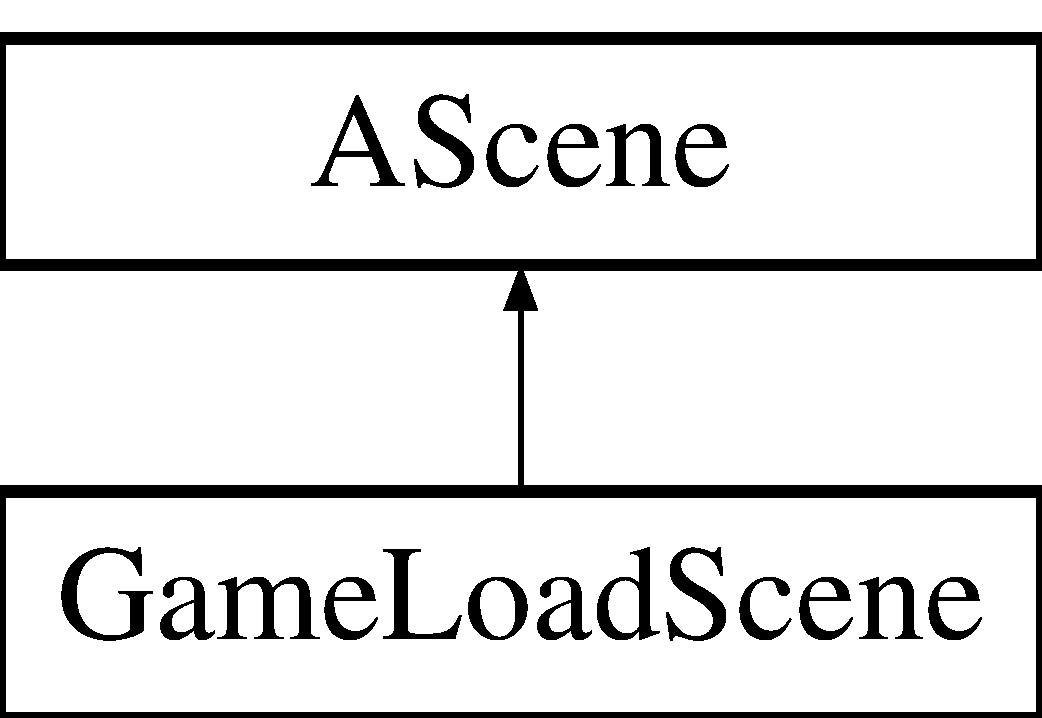
\includegraphics[height=2.000000cm]{classGameLoadScene}
\end{center}
\end{figure}
\subsection*{Public Member Functions}
\begin{DoxyCompactItemize}
\item 
\hyperlink{classGameLoadScene_a225786d3826577aa3743164b6262dc2b}{Game\+Load\+Scene} ()
\begin{DoxyCompactList}\small\item\em Constructor. \end{DoxyCompactList}\item 
\hyperlink{classGameLoadScene_a39c0f378455520c08d21e0642f35cd9b}{$\sim$\+Game\+Load\+Scene} ()
\begin{DoxyCompactList}\small\item\em Destructor. \end{DoxyCompactList}\item 
\mbox{\Hypertarget{classGameLoadScene_a4d2c3a0455cd070671dbef281b7bd87f}\label{classGameLoadScene_a4d2c3a0455cd070671dbef281b7bd87f}} 
void \hyperlink{classGameLoadScene_a4d2c3a0455cd070671dbef281b7bd87f}{prev} ()
\begin{DoxyCompactList}\small\item\em Pass to the prev scene. \end{DoxyCompactList}\item 
\mbox{\Hypertarget{classGameLoadScene_a67796257e428031f44010b9bf0b3173a}\label{classGameLoadScene_a67796257e428031f44010b9bf0b3173a}} 
void \hyperlink{classGameLoadScene_a67796257e428031f44010b9bf0b3173a}{print\+Current\+Save} ()
\begin{DoxyCompactList}\small\item\em Print current scene. \end{DoxyCompactList}\item 
\mbox{\Hypertarget{classGameLoadScene_aa00e2695ad042ee9a637ab0d5c08b054}\label{classGameLoadScene_aa00e2695ad042ee9a637ab0d5c08b054}} 
void \hyperlink{classGameLoadScene_aa00e2695ad042ee9a637ab0d5c08b054}{next} ()
\begin{DoxyCompactList}\small\item\em Pass to the next scene. \end{DoxyCompactList}\item 
irr\+::\+I\+Event\+Receiver $\ast$ \hyperlink{classGameLoadScene_a81807790ad65bd2cf97a1e543cae2b74}{get\+Event\+Receiver} () const
\begin{DoxyCompactList}\small\item\em Allow the user to implemente the event callback class for each scene. \end{DoxyCompactList}\end{DoxyCompactItemize}


\subsection{Detailed Description}
\hyperlink{classButton}{Button} interface of Game\+Load scene. 

\subsection{Constructor \& Destructor Documentation}
\mbox{\Hypertarget{classGameLoadScene_a225786d3826577aa3743164b6262dc2b}\label{classGameLoadScene_a225786d3826577aa3743164b6262dc2b}} 
\index{Game\+Load\+Scene@{Game\+Load\+Scene}!Game\+Load\+Scene@{Game\+Load\+Scene}}
\index{Game\+Load\+Scene@{Game\+Load\+Scene}!Game\+Load\+Scene@{Game\+Load\+Scene}}
\subsubsection{\texorpdfstring{Game\+Load\+Scene()}{GameLoadScene()}}
{\footnotesize\ttfamily Game\+Load\+Scene\+::\+Game\+Load\+Scene (\begin{DoxyParamCaption}{ }\end{DoxyParamCaption})}



Constructor. 

Build the class. \mbox{\Hypertarget{classGameLoadScene_a39c0f378455520c08d21e0642f35cd9b}\label{classGameLoadScene_a39c0f378455520c08d21e0642f35cd9b}} 
\index{Game\+Load\+Scene@{Game\+Load\+Scene}!````~Game\+Load\+Scene@{$\sim$\+Game\+Load\+Scene}}
\index{````~Game\+Load\+Scene@{$\sim$\+Game\+Load\+Scene}!Game\+Load\+Scene@{Game\+Load\+Scene}}
\subsubsection{\texorpdfstring{$\sim$\+Game\+Load\+Scene()}{~GameLoadScene()}}
{\footnotesize\ttfamily Game\+Load\+Scene\+::$\sim$\+Game\+Load\+Scene (\begin{DoxyParamCaption}{ }\end{DoxyParamCaption})}



Destructor. 

Destroy the class. 

\subsection{Member Function Documentation}
\mbox{\Hypertarget{classGameLoadScene_a81807790ad65bd2cf97a1e543cae2b74}\label{classGameLoadScene_a81807790ad65bd2cf97a1e543cae2b74}} 
\index{Game\+Load\+Scene@{Game\+Load\+Scene}!get\+Event\+Receiver@{get\+Event\+Receiver}}
\index{get\+Event\+Receiver@{get\+Event\+Receiver}!Game\+Load\+Scene@{Game\+Load\+Scene}}
\subsubsection{\texorpdfstring{get\+Event\+Receiver()}{getEventReceiver()}}
{\footnotesize\ttfamily irr\+::\+I\+Event\+Receiver $\ast$ Game\+Load\+Scene\+::get\+Event\+Receiver (\begin{DoxyParamCaption}{ }\end{DoxyParamCaption}) const\hspace{0.3cm}{\ttfamily [virtual]}}



Allow the user to implemente the event callback class for each scene. 

Return the event. 

Implements \hyperlink{classAScene_af521e5e6d30a5d2e5d30eb333e4d3abd}{A\+Scene}.



The documentation for this class was generated from the following files\+:\begin{DoxyCompactItemize}
\item 
inc/graphics/scenes/\hyperlink{GameLoadScene_8hh}{Game\+Load\+Scene.\+hh}\item 
src/graphics/scenes/Game\+Load\+Scene.\+cpp\end{DoxyCompactItemize}

\hypertarget{classGameMenuReceiver}{}\section{Game\+Menu\+Receiver Class Reference}
\label{classGameMenuReceiver}\index{Game\+Menu\+Receiver@{Game\+Menu\+Receiver}}


Manager of event of game scene.  




{\ttfamily \#include $<$Game\+Menu\+Receiver.\+hh$>$}



Inherits I\+Event\+Receiver.

\subsection*{Public Member Functions}
\begin{DoxyCompactItemize}
\item 
\hyperlink{classGameMenuReceiver_a5dd735dbdeddd9f11a999c9f0c4210e8}{Game\+Menu\+Receiver} ()
\begin{DoxyCompactList}\small\item\em Constructor. \end{DoxyCompactList}\item 
\hyperlink{classGameMenuReceiver_a490afacab72bebb8b1f28c3977f9ed44}{$\sim$\+Game\+Menu\+Receiver} ()
\begin{DoxyCompactList}\small\item\em Destructor. \end{DoxyCompactList}\item 
bool \hyperlink{classGameMenuReceiver_af6774556abc7e3718b7bf904cc62ead0}{On\+Event} (const irr\+::\+S\+Event \&event)
\begin{DoxyCompactList}\small\item\em Allow the user to handle envent into a scene. \end{DoxyCompactList}\end{DoxyCompactItemize}


\subsection{Detailed Description}
Manager of event of game scene. 

\subsection{Constructor \& Destructor Documentation}
\mbox{\Hypertarget{classGameMenuReceiver_a5dd735dbdeddd9f11a999c9f0c4210e8}\label{classGameMenuReceiver_a5dd735dbdeddd9f11a999c9f0c4210e8}} 
\index{Game\+Menu\+Receiver@{Game\+Menu\+Receiver}!Game\+Menu\+Receiver@{Game\+Menu\+Receiver}}
\index{Game\+Menu\+Receiver@{Game\+Menu\+Receiver}!Game\+Menu\+Receiver@{Game\+Menu\+Receiver}}
\subsubsection{\texorpdfstring{Game\+Menu\+Receiver()}{GameMenuReceiver()}}
{\footnotesize\ttfamily Game\+Menu\+Receiver\+::\+Game\+Menu\+Receiver (\begin{DoxyParamCaption}{ }\end{DoxyParamCaption})}



Constructor. 

Build the class. \mbox{\Hypertarget{classGameMenuReceiver_a490afacab72bebb8b1f28c3977f9ed44}\label{classGameMenuReceiver_a490afacab72bebb8b1f28c3977f9ed44}} 
\index{Game\+Menu\+Receiver@{Game\+Menu\+Receiver}!````~Game\+Menu\+Receiver@{$\sim$\+Game\+Menu\+Receiver}}
\index{````~Game\+Menu\+Receiver@{$\sim$\+Game\+Menu\+Receiver}!Game\+Menu\+Receiver@{Game\+Menu\+Receiver}}
\subsubsection{\texorpdfstring{$\sim$\+Game\+Menu\+Receiver()}{~GameMenuReceiver()}}
{\footnotesize\ttfamily Game\+Menu\+Receiver\+::$\sim$\+Game\+Menu\+Receiver (\begin{DoxyParamCaption}{ }\end{DoxyParamCaption})}



Destructor. 

Destroy the class. 

\subsection{Member Function Documentation}
\mbox{\Hypertarget{classGameMenuReceiver_af6774556abc7e3718b7bf904cc62ead0}\label{classGameMenuReceiver_af6774556abc7e3718b7bf904cc62ead0}} 
\index{Game\+Menu\+Receiver@{Game\+Menu\+Receiver}!On\+Event@{On\+Event}}
\index{On\+Event@{On\+Event}!Game\+Menu\+Receiver@{Game\+Menu\+Receiver}}
\subsubsection{\texorpdfstring{On\+Event()}{OnEvent()}}
{\footnotesize\ttfamily bool Game\+Menu\+Receiver\+::\+On\+Event (\begin{DoxyParamCaption}\item[{const irr\+::\+S\+Event \&}]{event }\end{DoxyParamCaption})}



Allow the user to handle envent into a scene. 

Return true if he know the event, false if not. 

The documentation for this class was generated from the following files\+:\begin{DoxyCompactItemize}
\item 
inc/graphics/scenes/events/\hyperlink{GameMenuReceiver_8hh}{Game\+Menu\+Receiver.\+hh}\item 
src/graphics/scenes/events/Game\+Menu\+Receiver.\+cpp\end{DoxyCompactItemize}

\hypertarget{classGameMenuScene}{}\section{Game\+Menu\+Scene Class Reference}
\label{classGameMenuScene}\index{Game\+Menu\+Scene@{Game\+Menu\+Scene}}


\hyperlink{classButton}{Button} interface of menu setting scene.  




{\ttfamily \#include $<$Game\+Menu\+Scene.\+hh$>$}

Inheritance diagram for Game\+Menu\+Scene\+:\begin{figure}[H]
\begin{center}
\leavevmode
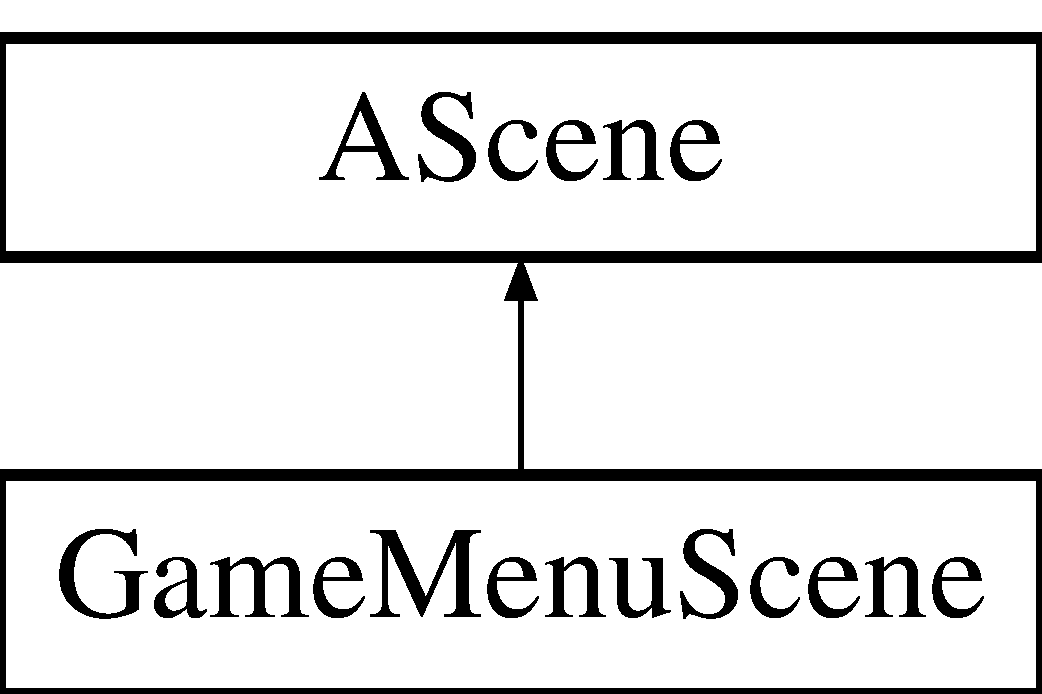
\includegraphics[height=2.000000cm]{classGameMenuScene}
\end{center}
\end{figure}
\subsection*{Public Member Functions}
\begin{DoxyCompactItemize}
\item 
\hyperlink{classGameMenuScene_a990633f8037ab2691f0aca251f3d89ee}{Game\+Menu\+Scene} ()
\begin{DoxyCompactList}\small\item\em Constructor. \end{DoxyCompactList}\item 
\hyperlink{classGameMenuScene_afbc6eddfe5f84b6f0b21bc652c9fc435}{$\sim$\+Game\+Menu\+Scene} ()
\begin{DoxyCompactList}\small\item\em Destructor. \end{DoxyCompactList}\item 
irr\+::\+I\+Event\+Receiver $\ast$ \hyperlink{classGameMenuScene_adcb01430b24486c4e5d0157fc32d7611}{get\+Event\+Receiver} () const
\begin{DoxyCompactList}\small\item\em Event getter. \end{DoxyCompactList}\end{DoxyCompactItemize}


\subsection{Detailed Description}
\hyperlink{classButton}{Button} interface of menu setting scene. 

\subsection{Constructor \& Destructor Documentation}
\mbox{\Hypertarget{classGameMenuScene_a990633f8037ab2691f0aca251f3d89ee}\label{classGameMenuScene_a990633f8037ab2691f0aca251f3d89ee}} 
\index{Game\+Menu\+Scene@{Game\+Menu\+Scene}!Game\+Menu\+Scene@{Game\+Menu\+Scene}}
\index{Game\+Menu\+Scene@{Game\+Menu\+Scene}!Game\+Menu\+Scene@{Game\+Menu\+Scene}}
\subsubsection{\texorpdfstring{Game\+Menu\+Scene()}{GameMenuScene()}}
{\footnotesize\ttfamily Game\+Menu\+Scene\+::\+Game\+Menu\+Scene (\begin{DoxyParamCaption}{ }\end{DoxyParamCaption})}



Constructor. 

Build the class. \mbox{\Hypertarget{classGameMenuScene_afbc6eddfe5f84b6f0b21bc652c9fc435}\label{classGameMenuScene_afbc6eddfe5f84b6f0b21bc652c9fc435}} 
\index{Game\+Menu\+Scene@{Game\+Menu\+Scene}!````~Game\+Menu\+Scene@{$\sim$\+Game\+Menu\+Scene}}
\index{````~Game\+Menu\+Scene@{$\sim$\+Game\+Menu\+Scene}!Game\+Menu\+Scene@{Game\+Menu\+Scene}}
\subsubsection{\texorpdfstring{$\sim$\+Game\+Menu\+Scene()}{~GameMenuScene()}}
{\footnotesize\ttfamily Game\+Menu\+Scene\+::$\sim$\+Game\+Menu\+Scene (\begin{DoxyParamCaption}{ }\end{DoxyParamCaption})}



Destructor. 

Destroy the class. 

\subsection{Member Function Documentation}
\mbox{\Hypertarget{classGameMenuScene_adcb01430b24486c4e5d0157fc32d7611}\label{classGameMenuScene_adcb01430b24486c4e5d0157fc32d7611}} 
\index{Game\+Menu\+Scene@{Game\+Menu\+Scene}!get\+Event\+Receiver@{get\+Event\+Receiver}}
\index{get\+Event\+Receiver@{get\+Event\+Receiver}!Game\+Menu\+Scene@{Game\+Menu\+Scene}}
\subsubsection{\texorpdfstring{get\+Event\+Receiver()}{getEventReceiver()}}
{\footnotesize\ttfamily irr\+::\+I\+Event\+Receiver $\ast$ Game\+Menu\+Scene\+::get\+Event\+Receiver (\begin{DoxyParamCaption}{ }\end{DoxyParamCaption}) const\hspace{0.3cm}{\ttfamily [virtual]}}



Event getter. 

Return the event. 

Implements \hyperlink{classAScene_af521e5e6d30a5d2e5d30eb333e4d3abd}{A\+Scene}.



The documentation for this class was generated from the following files\+:\begin{DoxyCompactItemize}
\item 
inc/graphics/scenes/\hyperlink{GameMenuScene_8hh}{Game\+Menu\+Scene.\+hh}\item 
src/graphics/scenes/Game\+Menu\+Scene.\+cpp\end{DoxyCompactItemize}

\hypertarget{classGameNewReceiver}{}\section{Game\+New\+Receiver Class Reference}
\label{classGameNewReceiver}\index{Game\+New\+Receiver@{Game\+New\+Receiver}}


Manager of event of new game scene.  




{\ttfamily \#include $<$Game\+New\+Receiver.\+hh$>$}

Inheritance diagram for Game\+New\+Receiver\+:\begin{figure}[H]
\begin{center}
\leavevmode
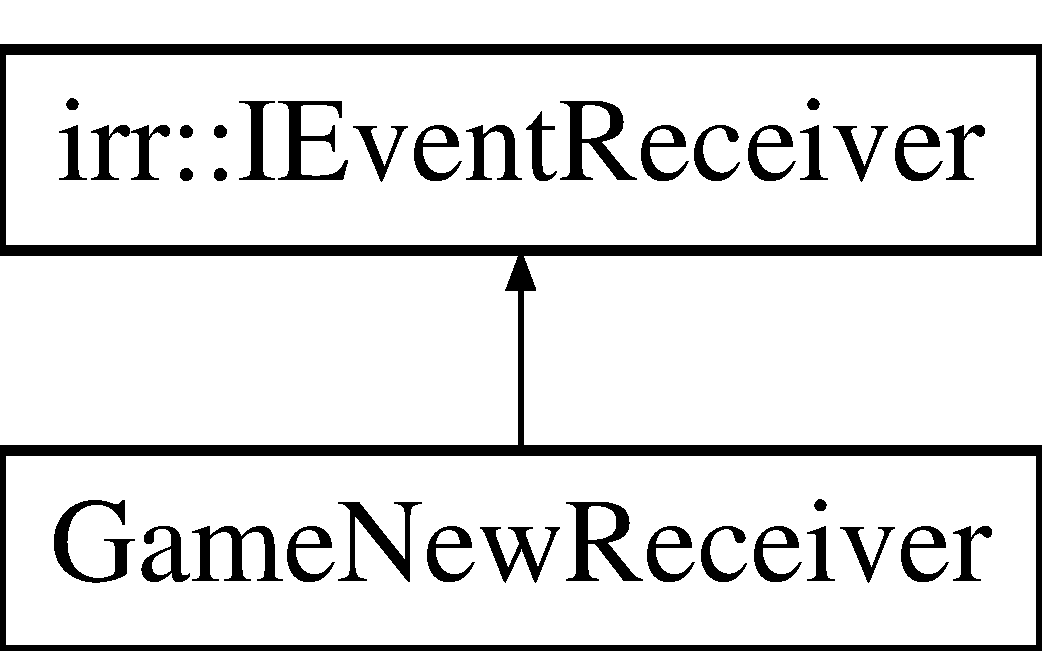
\includegraphics[height=2.000000cm]{classGameNewReceiver}
\end{center}
\end{figure}
\subsection*{Public Member Functions}
\begin{DoxyCompactItemize}
\item 
\hyperlink{classGameNewReceiver_a41816905e385ac8e17849d599106b930}{Game\+New\+Receiver} (const \hyperlink{classGameNewScene}{Game\+New\+Scene} $\ast$parent)
\begin{DoxyCompactList}\small\item\em Constructor. \end{DoxyCompactList}\item 
\hyperlink{classGameNewReceiver_ab92b6653b56d291853a4e2f737eaf6fd}{$\sim$\+Game\+New\+Receiver} ()
\begin{DoxyCompactList}\small\item\em Destructor. \end{DoxyCompactList}\item 
bool \hyperlink{classGameNewReceiver_ad9ec097d8b46946ed1a21c24463fc0b6}{On\+Event} (const \hyperlink{structirr_1_1SEvent}{irr\+::\+S\+Event} \&event)
\begin{DoxyCompactList}\small\item\em Allow the user to handle envent into a scene. \end{DoxyCompactList}\end{DoxyCompactItemize}


\subsection{Detailed Description}
Manager of event of new game scene. 

\subsection{Constructor \& Destructor Documentation}
\mbox{\Hypertarget{classGameNewReceiver_a41816905e385ac8e17849d599106b930}\label{classGameNewReceiver_a41816905e385ac8e17849d599106b930}} 
\index{Game\+New\+Receiver@{Game\+New\+Receiver}!Game\+New\+Receiver@{Game\+New\+Receiver}}
\index{Game\+New\+Receiver@{Game\+New\+Receiver}!Game\+New\+Receiver@{Game\+New\+Receiver}}
\subsubsection{\texorpdfstring{Game\+New\+Receiver()}{GameNewReceiver()}}
{\footnotesize\ttfamily Game\+New\+Receiver\+::\+Game\+New\+Receiver (\begin{DoxyParamCaption}\item[{const \hyperlink{classGameNewScene}{Game\+New\+Scene} $\ast$}]{parent }\end{DoxyParamCaption})}



Constructor. 

Build the class. \mbox{\Hypertarget{classGameNewReceiver_ab92b6653b56d291853a4e2f737eaf6fd}\label{classGameNewReceiver_ab92b6653b56d291853a4e2f737eaf6fd}} 
\index{Game\+New\+Receiver@{Game\+New\+Receiver}!````~Game\+New\+Receiver@{$\sim$\+Game\+New\+Receiver}}
\index{````~Game\+New\+Receiver@{$\sim$\+Game\+New\+Receiver}!Game\+New\+Receiver@{Game\+New\+Receiver}}
\subsubsection{\texorpdfstring{$\sim$\+Game\+New\+Receiver()}{~GameNewReceiver()}}
{\footnotesize\ttfamily Game\+New\+Receiver\+::$\sim$\+Game\+New\+Receiver (\begin{DoxyParamCaption}{ }\end{DoxyParamCaption})}



Destructor. 

Destroy the class. 

\subsection{Member Function Documentation}
\mbox{\Hypertarget{classGameNewReceiver_ad9ec097d8b46946ed1a21c24463fc0b6}\label{classGameNewReceiver_ad9ec097d8b46946ed1a21c24463fc0b6}} 
\index{Game\+New\+Receiver@{Game\+New\+Receiver}!On\+Event@{On\+Event}}
\index{On\+Event@{On\+Event}!Game\+New\+Receiver@{Game\+New\+Receiver}}
\subsubsection{\texorpdfstring{On\+Event()}{OnEvent()}}
{\footnotesize\ttfamily bool Game\+New\+Receiver\+::\+On\+Event (\begin{DoxyParamCaption}\item[{const \hyperlink{structirr_1_1SEvent}{irr\+::\+S\+Event} \&}]{event }\end{DoxyParamCaption})\hspace{0.3cm}{\ttfamily [virtual]}}



Allow the user to handle envent into a scene. 

Return true if he know the event, false if not. 

Implements \hyperlink{classirr_1_1IEventReceiver_a571f744ceffc3b4fe8a81f529163eb97}{irr\+::\+I\+Event\+Receiver}.



The documentation for this class was generated from the following files\+:\begin{DoxyCompactItemize}
\item 
inc/graphics/scenes/events/\hyperlink{GameNewReceiver_8hh}{Game\+New\+Receiver.\+hh}\item 
src/graphics/scenes/events/Game\+New\+Receiver.\+cpp\end{DoxyCompactItemize}

\hypertarget{classGameNewScene}{}\section{Game\+New\+Scene Class Reference}
\label{classGameNewScene}\index{Game\+New\+Scene@{Game\+New\+Scene}}


\hyperlink{classButton}{Button} interface of new game setting scene.  




{\ttfamily \#include $<$Game\+New\+Scene.\+hh$>$}

Inheritance diagram for Game\+New\+Scene\+:\begin{figure}[H]
\begin{center}
\leavevmode
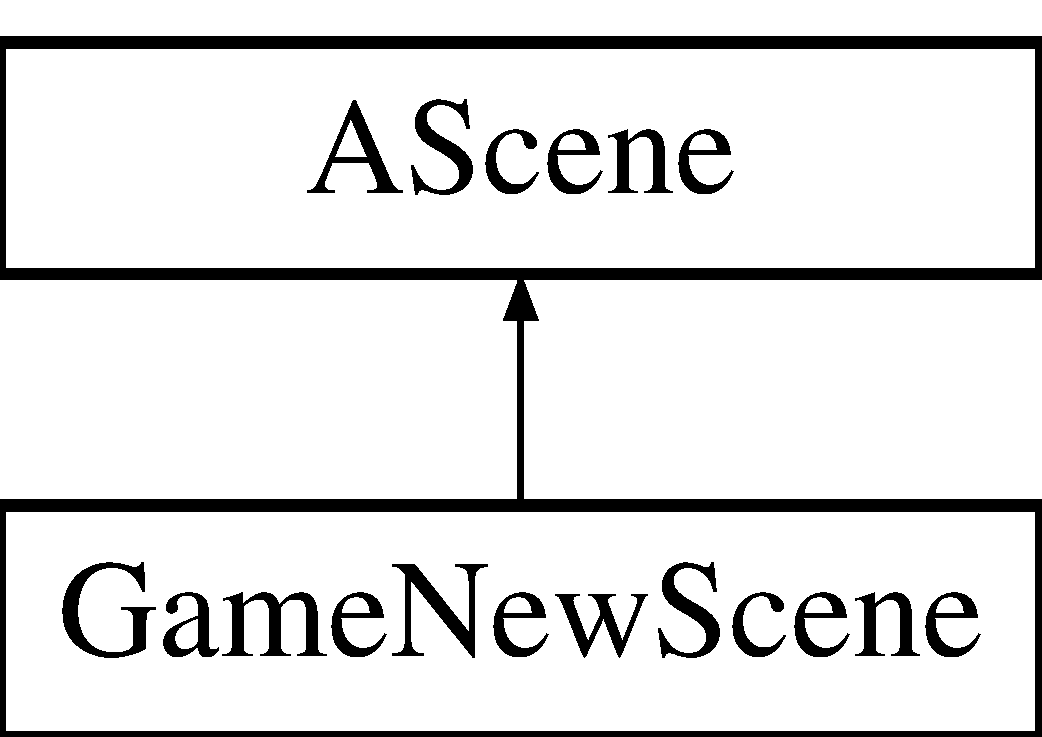
\includegraphics[height=2.000000cm]{classGameNewScene}
\end{center}
\end{figure}
\subsection*{Public Member Functions}
\begin{DoxyCompactItemize}
\item 
\hyperlink{classGameNewScene_af482b13a2d9e315ef39a6e41293bf4fb}{Game\+New\+Scene} ()
\begin{DoxyCompactList}\small\item\em Constructor. \end{DoxyCompactList}\item 
\hyperlink{classGameNewScene_a3df0ff81012d3f7dbd08c7367be22fdf}{$\sim$\+Game\+New\+Scene} ()
\begin{DoxyCompactList}\small\item\em Destructor. \end{DoxyCompactList}\item 
irr\+::\+I\+Event\+Receiver $\ast$ \hyperlink{classGameNewScene_a21c27ef3ea1923d975683e1bcdd134fa}{get\+Event\+Receiver} () const
\begin{DoxyCompactList}\small\item\em Allow the user to implemente the event callback class for each scene. \end{DoxyCompactList}\item 
\mbox{\Hypertarget{classGameNewScene_a2fb7cacfacbf5c565c3e2f98bd06aec4}\label{classGameNewScene_a2fb7cacfacbf5c565c3e2f98bd06aec4}} 
std\+::vector$<$ std\+::shared\+\_\+ptr$<$ A\+Hero $>$ $>$ \& \hyperlink{classGameNewScene_a2fb7cacfacbf5c565c3e2f98bd06aec4}{get\+Players} ()
\begin{DoxyCompactList}\small\item\em Return the players table. \end{DoxyCompactList}\item 
\mbox{\Hypertarget{classGameNewScene_a8ec7d1675e6be7490aee15126d8f2026}\label{classGameNewScene_a8ec7d1675e6be7490aee15126d8f2026}} 
std\+::vector$<$ std\+::shared\+\_\+ptr$<$ Player\+Configuration $>$ $>$ \& \hyperlink{classGameNewScene_a8ec7d1675e6be7490aee15126d8f2026}{get\+Players\+Configurations} ()
\begin{DoxyCompactList}\small\item\em Return the players configurations. \end{DoxyCompactList}\end{DoxyCompactItemize}


\subsection{Detailed Description}
\hyperlink{classButton}{Button} interface of new game setting scene. 

\subsection{Constructor \& Destructor Documentation}
\mbox{\Hypertarget{classGameNewScene_af482b13a2d9e315ef39a6e41293bf4fb}\label{classGameNewScene_af482b13a2d9e315ef39a6e41293bf4fb}} 
\index{Game\+New\+Scene@{Game\+New\+Scene}!Game\+New\+Scene@{Game\+New\+Scene}}
\index{Game\+New\+Scene@{Game\+New\+Scene}!Game\+New\+Scene@{Game\+New\+Scene}}
\subsubsection{\texorpdfstring{Game\+New\+Scene()}{GameNewScene()}}
{\footnotesize\ttfamily Game\+New\+Scene\+::\+Game\+New\+Scene (\begin{DoxyParamCaption}{ }\end{DoxyParamCaption})}



Constructor. 

Build the class. \mbox{\Hypertarget{classGameNewScene_a3df0ff81012d3f7dbd08c7367be22fdf}\label{classGameNewScene_a3df0ff81012d3f7dbd08c7367be22fdf}} 
\index{Game\+New\+Scene@{Game\+New\+Scene}!````~Game\+New\+Scene@{$\sim$\+Game\+New\+Scene}}
\index{````~Game\+New\+Scene@{$\sim$\+Game\+New\+Scene}!Game\+New\+Scene@{Game\+New\+Scene}}
\subsubsection{\texorpdfstring{$\sim$\+Game\+New\+Scene()}{~GameNewScene()}}
{\footnotesize\ttfamily Game\+New\+Scene\+::$\sim$\+Game\+New\+Scene (\begin{DoxyParamCaption}{ }\end{DoxyParamCaption})}



Destructor. 

Destroy the class. 

\subsection{Member Function Documentation}
\mbox{\Hypertarget{classGameNewScene_a21c27ef3ea1923d975683e1bcdd134fa}\label{classGameNewScene_a21c27ef3ea1923d975683e1bcdd134fa}} 
\index{Game\+New\+Scene@{Game\+New\+Scene}!get\+Event\+Receiver@{get\+Event\+Receiver}}
\index{get\+Event\+Receiver@{get\+Event\+Receiver}!Game\+New\+Scene@{Game\+New\+Scene}}
\subsubsection{\texorpdfstring{get\+Event\+Receiver()}{getEventReceiver()}}
{\footnotesize\ttfamily irr\+::\+I\+Event\+Receiver $\ast$ Game\+New\+Scene\+::get\+Event\+Receiver (\begin{DoxyParamCaption}{ }\end{DoxyParamCaption}) const\hspace{0.3cm}{\ttfamily [virtual]}}



Allow the user to implemente the event callback class for each scene. 

Return the event. 

Implements \hyperlink{classAScene_af521e5e6d30a5d2e5d30eb333e4d3abd}{A\+Scene}.



The documentation for this class was generated from the following files\+:\begin{DoxyCompactItemize}
\item 
inc/graphics/scenes/\hyperlink{GameNewScene_8hh}{Game\+New\+Scene.\+hh}\item 
src/graphics/scenes/Game\+New\+Scene.\+cpp\end{DoxyCompactItemize}

\hypertarget{classGameOnlineScene}{}\section{Game\+Online\+Scene Class Reference}
\label{classGameOnlineScene}\index{Game\+Online\+Scene@{Game\+Online\+Scene}}


\hyperlink{classButton}{Button} interface of Game\+Onlinescene.  




{\ttfamily \#include $<$Game\+Online\+Scene.\+hh$>$}

Inheritance diagram for Game\+Online\+Scene\+:\begin{figure}[H]
\begin{center}
\leavevmode
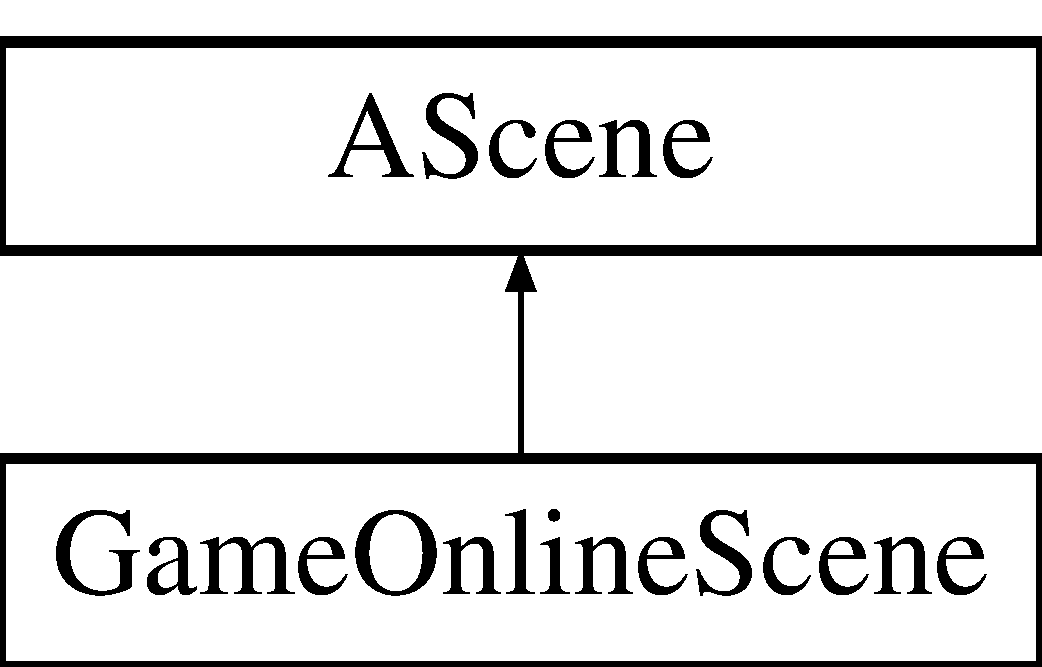
\includegraphics[height=2.000000cm]{classGameOnlineScene}
\end{center}
\end{figure}
\subsection*{Public Member Functions}
\begin{DoxyCompactItemize}
\item 
\hyperlink{classGameOnlineScene_a057362d043c386aa2b6789baf548fa09}{Game\+Online\+Scene} ()
\begin{DoxyCompactList}\small\item\em Constructor. \end{DoxyCompactList}\item 
\hyperlink{classGameOnlineScene_a59b127983ae2338edcf0b8bd86ff9f96}{$\sim$\+Game\+Online\+Scene} ()
\begin{DoxyCompactList}\small\item\em Destructor. \end{DoxyCompactList}\item 
irr\+::\+I\+Event\+Receiver $\ast$ \hyperlink{classGameOnlineScene_a00ce9773db4f1886fc463b023cbf63f9}{get\+Event\+Receiver} () const
\begin{DoxyCompactList}\small\item\em Allow the user to implemente the event callback class for each scene. \end{DoxyCompactList}\end{DoxyCompactItemize}


\subsection{Detailed Description}
\hyperlink{classButton}{Button} interface of Game\+Onlinescene. 

\subsection{Constructor \& Destructor Documentation}
\mbox{\Hypertarget{classGameOnlineScene_a057362d043c386aa2b6789baf548fa09}\label{classGameOnlineScene_a057362d043c386aa2b6789baf548fa09}} 
\index{Game\+Online\+Scene@{Game\+Online\+Scene}!Game\+Online\+Scene@{Game\+Online\+Scene}}
\index{Game\+Online\+Scene@{Game\+Online\+Scene}!Game\+Online\+Scene@{Game\+Online\+Scene}}
\subsubsection{\texorpdfstring{Game\+Online\+Scene()}{GameOnlineScene()}}
{\footnotesize\ttfamily Game\+Online\+Scene\+::\+Game\+Online\+Scene (\begin{DoxyParamCaption}{ }\end{DoxyParamCaption})}



Constructor. 

Build the class. \mbox{\Hypertarget{classGameOnlineScene_a59b127983ae2338edcf0b8bd86ff9f96}\label{classGameOnlineScene_a59b127983ae2338edcf0b8bd86ff9f96}} 
\index{Game\+Online\+Scene@{Game\+Online\+Scene}!````~Game\+Online\+Scene@{$\sim$\+Game\+Online\+Scene}}
\index{````~Game\+Online\+Scene@{$\sim$\+Game\+Online\+Scene}!Game\+Online\+Scene@{Game\+Online\+Scene}}
\subsubsection{\texorpdfstring{$\sim$\+Game\+Online\+Scene()}{~GameOnlineScene()}}
{\footnotesize\ttfamily Game\+Online\+Scene\+::$\sim$\+Game\+Online\+Scene (\begin{DoxyParamCaption}{ }\end{DoxyParamCaption})}



Destructor. 

Destroy the class. 

\subsection{Member Function Documentation}
\mbox{\Hypertarget{classGameOnlineScene_a00ce9773db4f1886fc463b023cbf63f9}\label{classGameOnlineScene_a00ce9773db4f1886fc463b023cbf63f9}} 
\index{Game\+Online\+Scene@{Game\+Online\+Scene}!get\+Event\+Receiver@{get\+Event\+Receiver}}
\index{get\+Event\+Receiver@{get\+Event\+Receiver}!Game\+Online\+Scene@{Game\+Online\+Scene}}
\subsubsection{\texorpdfstring{get\+Event\+Receiver()}{getEventReceiver()}}
{\footnotesize\ttfamily irr\+::\+I\+Event\+Receiver $\ast$ Game\+Online\+Scene\+::get\+Event\+Receiver (\begin{DoxyParamCaption}{ }\end{DoxyParamCaption}) const\hspace{0.3cm}{\ttfamily [virtual]}}



Allow the user to implemente the event callback class for each scene. 

Return the event. 

Implements \hyperlink{classAScene_af521e5e6d30a5d2e5d30eb333e4d3abd}{A\+Scene}.



The documentation for this class was generated from the following files\+:\begin{DoxyCompactItemize}
\item 
inc/graphics/scenes/\hyperlink{GameOnlineScene_8hh}{Game\+Online\+Scene.\+hh}\item 
src/graphics/scenes/Game\+Online\+Scene.\+cpp\end{DoxyCompactItemize}

\hypertarget{classGameSimulationScene}{}\section{Game\+Simulation\+Scene Class Reference}
\label{classGameSimulationScene}\index{Game\+Simulation\+Scene@{Game\+Simulation\+Scene}}


\hyperlink{classButton}{Button} interface of Game\+Simulationscene.  




{\ttfamily \#include $<$Game\+Simulation\+Scene.\+hh$>$}

Inheritance diagram for Game\+Simulation\+Scene\+:\begin{figure}[H]
\begin{center}
\leavevmode
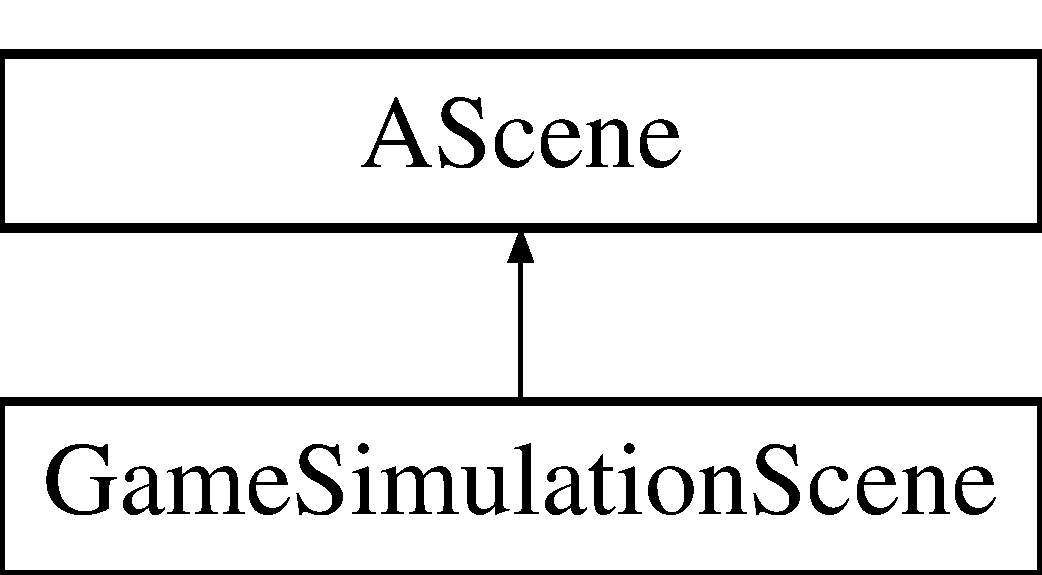
\includegraphics[height=2.000000cm]{classGameSimulationScene}
\end{center}
\end{figure}
\subsection*{Public Member Functions}
\begin{DoxyCompactItemize}
\item 
\hyperlink{classGameSimulationScene_a6983b2c511d45278121bcf62151fbb19}{Game\+Simulation\+Scene} (const std\+::shared\+\_\+ptr$<$ \hyperlink{classLevel}{Level} $>$ \&level)
\begin{DoxyCompactList}\small\item\em Constructor. \end{DoxyCompactList}\item 
\hyperlink{classGameSimulationScene_af45f3e7f70376e59a6f320f21ce2897b}{$\sim$\+Game\+Simulation\+Scene} ()
\begin{DoxyCompactList}\small\item\em Destructor. \end{DoxyCompactList}\item 
void \hyperlink{classGameSimulationScene_a66b107f708b5eed87a3c0a0016541d29}{update\+Camera} (\hyperlink{classWindow}{Window} $\ast$win)
\begin{DoxyCompactList}\small\item\em Update camera\textquotesingle{}s position. \end{DoxyCompactList}\item 
\hyperlink{classirr_1_1IEventReceiver}{irr\+::\+I\+Event\+Receiver} $\ast$ \hyperlink{classGameSimulationScene_a048b2a937caff3af7b4d54f8bd404ec1}{get\+Event\+Receiver} () const
\begin{DoxyCompactList}\small\item\em Allow the user to implemente the event callback class for each scene. \end{DoxyCompactList}\end{DoxyCompactItemize}


\subsection{Detailed Description}
\hyperlink{classButton}{Button} interface of Game\+Simulationscene. 

\subsection{Constructor \& Destructor Documentation}
\mbox{\Hypertarget{classGameSimulationScene_a6983b2c511d45278121bcf62151fbb19}\label{classGameSimulationScene_a6983b2c511d45278121bcf62151fbb19}} 
\index{Game\+Simulation\+Scene@{Game\+Simulation\+Scene}!Game\+Simulation\+Scene@{Game\+Simulation\+Scene}}
\index{Game\+Simulation\+Scene@{Game\+Simulation\+Scene}!Game\+Simulation\+Scene@{Game\+Simulation\+Scene}}
\subsubsection{\texorpdfstring{Game\+Simulation\+Scene()}{GameSimulationScene()}}
{\footnotesize\ttfamily Game\+Simulation\+Scene\+::\+Game\+Simulation\+Scene (\begin{DoxyParamCaption}\item[{const std\+::shared\+\_\+ptr$<$ \hyperlink{classLevel}{Level} $>$ \&}]{level }\end{DoxyParamCaption})}



Constructor. 

Build the class. \mbox{\Hypertarget{classGameSimulationScene_af45f3e7f70376e59a6f320f21ce2897b}\label{classGameSimulationScene_af45f3e7f70376e59a6f320f21ce2897b}} 
\index{Game\+Simulation\+Scene@{Game\+Simulation\+Scene}!````~Game\+Simulation\+Scene@{$\sim$\+Game\+Simulation\+Scene}}
\index{````~Game\+Simulation\+Scene@{$\sim$\+Game\+Simulation\+Scene}!Game\+Simulation\+Scene@{Game\+Simulation\+Scene}}
\subsubsection{\texorpdfstring{$\sim$\+Game\+Simulation\+Scene()}{~GameSimulationScene()}}
{\footnotesize\ttfamily Game\+Simulation\+Scene\+::$\sim$\+Game\+Simulation\+Scene (\begin{DoxyParamCaption}{ }\end{DoxyParamCaption})}



Destructor. 

Destroy the class. 

\subsection{Member Function Documentation}
\mbox{\Hypertarget{classGameSimulationScene_a048b2a937caff3af7b4d54f8bd404ec1}\label{classGameSimulationScene_a048b2a937caff3af7b4d54f8bd404ec1}} 
\index{Game\+Simulation\+Scene@{Game\+Simulation\+Scene}!get\+Event\+Receiver@{get\+Event\+Receiver}}
\index{get\+Event\+Receiver@{get\+Event\+Receiver}!Game\+Simulation\+Scene@{Game\+Simulation\+Scene}}
\subsubsection{\texorpdfstring{get\+Event\+Receiver()}{getEventReceiver()}}
{\footnotesize\ttfamily \hyperlink{classirr_1_1IEventReceiver}{irr\+::\+I\+Event\+Receiver} $\ast$ Game\+Simulation\+Scene\+::get\+Event\+Receiver (\begin{DoxyParamCaption}{ }\end{DoxyParamCaption}) const\hspace{0.3cm}{\ttfamily [virtual]}}



Allow the user to implemente the event callback class for each scene. 

Return the event. 

Implements \hyperlink{classAScene_af521e5e6d30a5d2e5d30eb333e4d3abd}{A\+Scene}.

\mbox{\Hypertarget{classGameSimulationScene_a66b107f708b5eed87a3c0a0016541d29}\label{classGameSimulationScene_a66b107f708b5eed87a3c0a0016541d29}} 
\index{Game\+Simulation\+Scene@{Game\+Simulation\+Scene}!update\+Camera@{update\+Camera}}
\index{update\+Camera@{update\+Camera}!Game\+Simulation\+Scene@{Game\+Simulation\+Scene}}
\subsubsection{\texorpdfstring{update\+Camera()}{updateCamera()}}
{\footnotesize\ttfamily void Game\+Simulation\+Scene\+::update\+Camera (\begin{DoxyParamCaption}\item[{\hyperlink{classWindow}{Window} $\ast$}]{win }\end{DoxyParamCaption})\hspace{0.3cm}{\ttfamily [virtual]}}



Update camera\textquotesingle{}s position. 


\begin{DoxyParams}{Parameters}
{\em The} & window who contain the camera. \\
\hline
\end{DoxyParams}


Reimplemented from \hyperlink{classAScene_a18070899d965f1811c2253ad1d939374}{A\+Scene}.



The documentation for this class was generated from the following files\+:\begin{DoxyCompactItemize}
\item 
inc/graphics/scenes/\hyperlink{GameSimulationScene_8hh}{Game\+Simulation\+Scene.\+hh}\item 
src/graphics/scenes/Game\+Simulation\+Scene.\+cpp\end{DoxyCompactItemize}

\hypertarget{classGravity}{}\section{Gravity Class Reference}
\label{classGravity}\index{Gravity@{Gravity}}


where \hyperlink{classGravity}{Gravity} behaviour is defined  




{\ttfamily \#include $<$Gravity.\+hh$>$}

\subsection*{Public Member Functions}
\begin{DoxyCompactItemize}
\item 
\mbox{\Hypertarget{classGravity_ae971708aa344811adcc352e2d8a707de}\label{classGravity_ae971708aa344811adcc352e2d8a707de}} 
\hyperlink{classGravity_ae971708aa344811adcc352e2d8a707de}{Gravity} ()
\begin{DoxyCompactList}\small\item\em Instanciate \hyperlink{classGravity}{Gravity}. \end{DoxyCompactList}\item 
\mbox{\Hypertarget{classGravity_a6fcaf5f5f0d4672c4a1d97a3102e053a}\label{classGravity_a6fcaf5f5f0d4672c4a1d97a3102e053a}} 
\hyperlink{classGravity_a6fcaf5f5f0d4672c4a1d97a3102e053a}{$\sim$\+Gravity} ()
\begin{DoxyCompactList}\small\item\em Destructor. \end{DoxyCompactList}\item 
void \hyperlink{classGravity_adc8738cabe1e73c29697f7065d1273e0}{set\+Gravity} (irr\+::scene\+::\+I\+Animated\+Mesh\+Scene\+Node $\ast$node, const irr\+::core\+::vector3df \&elipsoid\+Radius=irr\+::core\+::vector3df(30, 60, 30), const irr\+::core\+::vector3df \&gravity\+Per\+Second=irr\+::core\+::vector3df(0,-\/10.\+0f, 0))
\begin{DoxyCompactList}\small\item\em set\+Gravity apply gravity to given mesh \end{DoxyCompactList}\item 
\mbox{\Hypertarget{classGravity_a2e27a01c3edd1a5d8aa580dced3c92b8}\label{classGravity_a2e27a01c3edd1a5d8aa580dced3c92b8}} 
void \hyperlink{classGravity_a2e27a01c3edd1a5d8aa580dced3c92b8}{unset\+Gravity} ()
\begin{DoxyCompactList}\small\item\em unset\+Gravity unset gravity of given mesh \end{DoxyCompactList}\end{DoxyCompactItemize}


\subsection{Detailed Description}
where \hyperlink{classGravity}{Gravity} behaviour is defined 

\subsection{Member Function Documentation}
\mbox{\Hypertarget{classGravity_adc8738cabe1e73c29697f7065d1273e0}\label{classGravity_adc8738cabe1e73c29697f7065d1273e0}} 
\index{Gravity@{Gravity}!set\+Gravity@{set\+Gravity}}
\index{set\+Gravity@{set\+Gravity}!Gravity@{Gravity}}
\subsubsection{\texorpdfstring{set\+Gravity()}{setGravity()}}
{\footnotesize\ttfamily void Gravity\+::set\+Gravity (\begin{DoxyParamCaption}\item[{irr\+::scene\+::\+I\+Animated\+Mesh\+Scene\+Node $\ast$}]{node,  }\item[{const irr\+::core\+::vector3df \&}]{elipsoid\+Radius = {\ttfamily irr\+:\+:core\+:\+:vector3df(30,60,30)},  }\item[{const irr\+::core\+::vector3df \&}]{gravity\+Per\+Second = {\ttfamily irr\+:\+:core\+:\+:vector3df(0,-\/10.0f,0)} }\end{DoxyParamCaption})}



set\+Gravity apply gravity to given mesh 


\begin{DoxyParams}{Parameters}
{\em node} & Node to which you want to apply gravity \\
\hline
{\em elipsoid\+Radius} & Elipsoid radius \\
\hline
{\em gravity\+Per\+Second} & \hyperlink{classGravity}{Gravity} (x,y,z) which will be apply to the given node \\
\hline
\end{DoxyParams}


The documentation for this class was generated from the following files\+:\begin{DoxyCompactItemize}
\item 
inc/graphics/\hyperlink{Gravity_8hh}{Gravity.\+hh}\item 
src/graphics/Gravity.\+cpp\end{DoxyCompactItemize}

\hypertarget{classImage}{}\section{Image Class Reference}
\label{classImage}\index{Image@{Image}}


Represent a image in the user interface.  




{\ttfamily \#include $<$Image.\+hh$>$}

Inheritance diagram for Image\+:\begin{figure}[H]
\begin{center}
\leavevmode
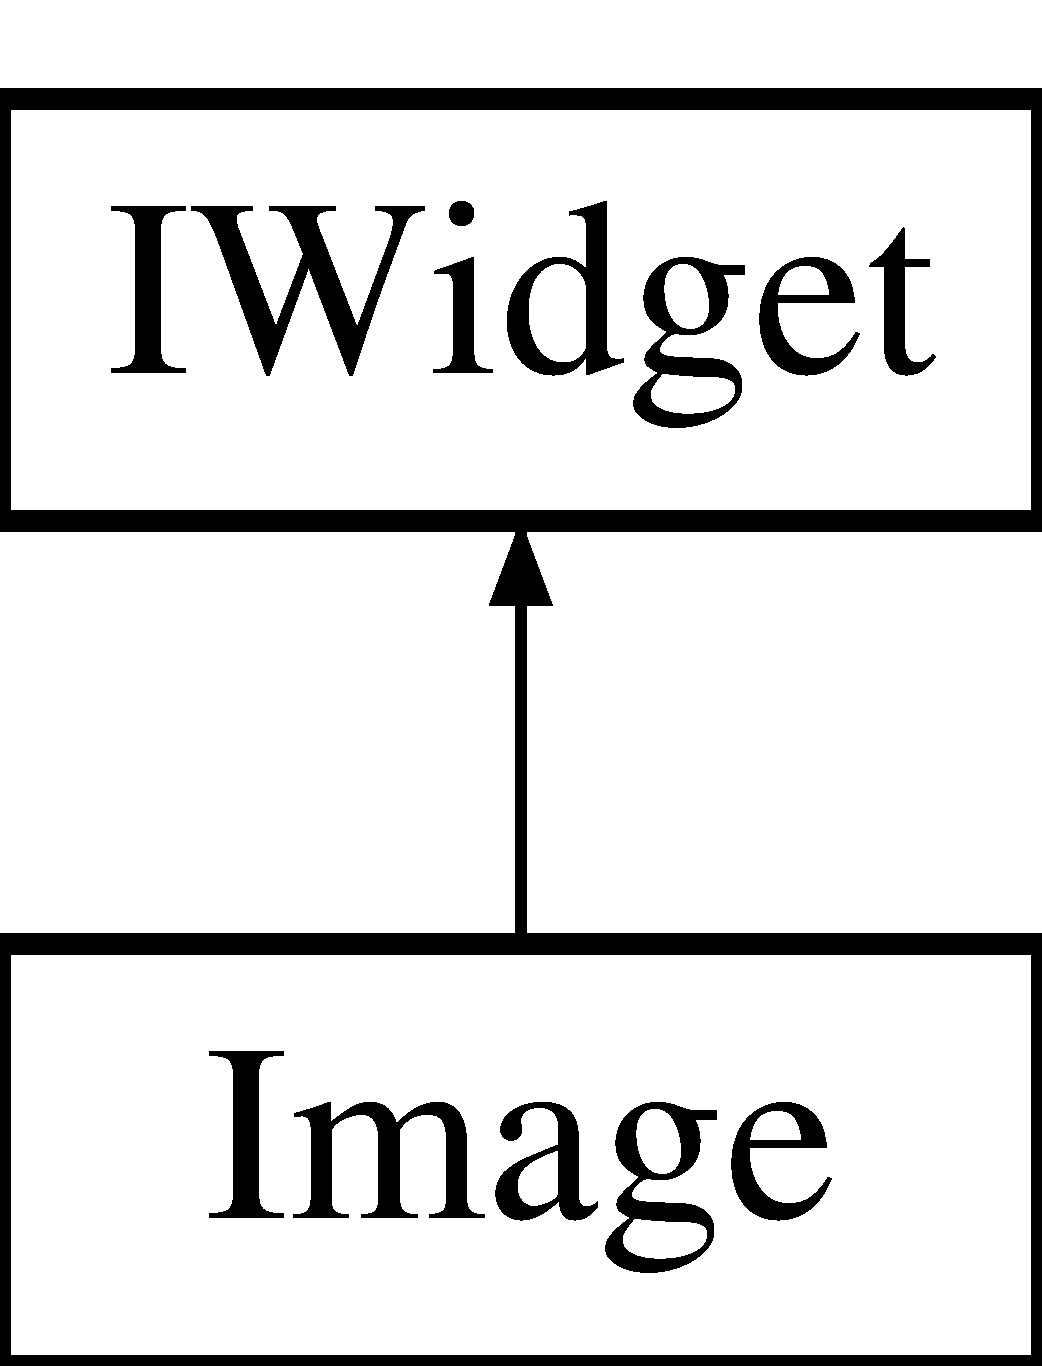
\includegraphics[height=2.000000cm]{classImage}
\end{center}
\end{figure}
\subsection*{Public Member Functions}
\begin{DoxyCompactItemize}
\item 
\hyperlink{classImage_aca308a45e7c53ec95e244863cb31a738}{Image} (const String \&name, const Position2d \&pos)
\begin{DoxyCompactList}\small\item\em Constructor. \end{DoxyCompactList}\item 
\mbox{\Hypertarget{classImage_a0294f63700543e11c0f0da85601c7ae5}\label{classImage_a0294f63700543e11c0f0da85601c7ae5}} 
\hyperlink{classImage_a0294f63700543e11c0f0da85601c7ae5}{$\sim$\+Image} ()
\begin{DoxyCompactList}\small\item\em Destructor. \end{DoxyCompactList}\item 
\mbox{\Hypertarget{classImage_a1c98ca475ce45aaa71e8a91a2a781ff5}\label{classImage_a1c98ca475ce45aaa71e8a91a2a781ff5}} 
void \hyperlink{classImage_a1c98ca475ce45aaa71e8a91a2a781ff5}{print} ()
\begin{DoxyCompactList}\small\item\em Print the image into the window. \end{DoxyCompactList}\item 
\mbox{\Hypertarget{classImage_a8a781889a88d1757620c61501d24d394}\label{classImage_a8a781889a88d1757620c61501d24d394}} 
void \hyperlink{classImage_a8a781889a88d1757620c61501d24d394}{set\+Position} (const Position2d \&pos)
\begin{DoxyCompactList}\small\item\em Set the image\textquotesingle{}s position. \end{DoxyCompactList}\end{DoxyCompactItemize}


\subsection{Detailed Description}
Represent a image in the user interface. 

\subsection{Constructor \& Destructor Documentation}
\mbox{\Hypertarget{classImage_aca308a45e7c53ec95e244863cb31a738}\label{classImage_aca308a45e7c53ec95e244863cb31a738}} 
\index{Image@{Image}!Image@{Image}}
\index{Image@{Image}!Image@{Image}}
\subsubsection{\texorpdfstring{Image()}{Image()}}
{\footnotesize\ttfamily Image\+::\+Image (\begin{DoxyParamCaption}\item[{const String \&}]{name,  }\item[{const Position2d \&}]{pos }\end{DoxyParamCaption})}



Constructor. 


\begin{DoxyParams}{Parameters}
{\em name} & The name of the image that will be load and print. \\
\hline
{\em pos} & The position of the image where the image will be print. \\
\hline
\end{DoxyParams}


The documentation for this class was generated from the following files\+:\begin{DoxyCompactItemize}
\item 
inc/graphics/widgets/\hyperlink{Image_8hh}{Image.\+hh}\item 
src/graphics/widgets/Image.\+cpp\end{DoxyCompactItemize}

\hypertarget{classIntroScene}{}\section{Intro\+Scene Class Reference}
\label{classIntroScene}\index{Intro\+Scene@{Intro\+Scene}}


\hyperlink{classButton}{Button} interface of Introcene.  




{\ttfamily \#include $<$Intro\+Scene.\+hh$>$}

Inheritance diagram for Intro\+Scene\+:\begin{figure}[H]
\begin{center}
\leavevmode
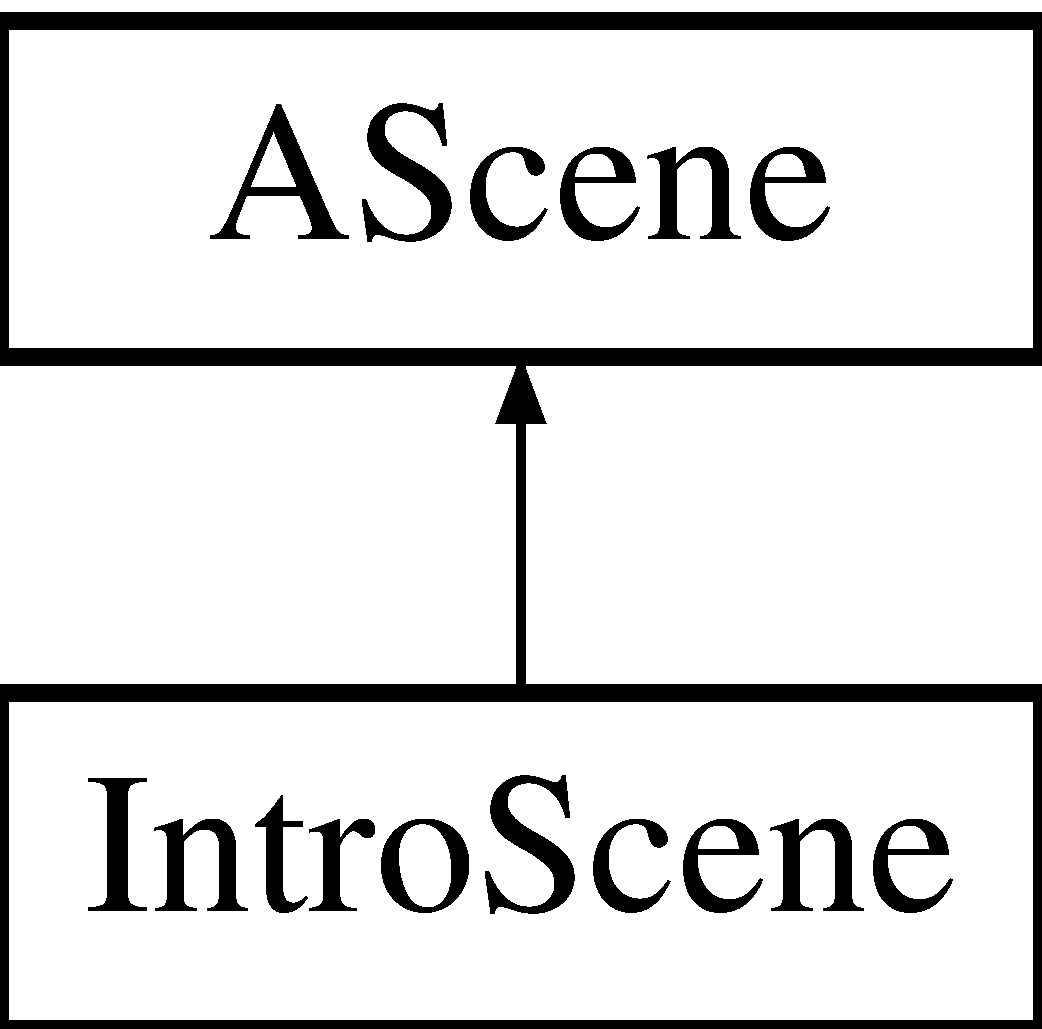
\includegraphics[height=2.000000cm]{classIntroScene}
\end{center}
\end{figure}
\subsection*{Public Member Functions}
\begin{DoxyCompactItemize}
\item 
\hyperlink{classIntroScene_a3691b51409f65b40f0c84008e49ef32b}{Intro\+Scene} ()
\begin{DoxyCompactList}\small\item\em Constructor. \end{DoxyCompactList}\item 
\hyperlink{classIntroScene_a7cdb50b55c0f5cf66b7bd151e4abe2b1}{$\sim$\+Intro\+Scene} ()
\begin{DoxyCompactList}\small\item\em Destructor. \end{DoxyCompactList}\item 
\hyperlink{classirr_1_1IEventReceiver}{irr\+::\+I\+Event\+Receiver} $\ast$ \hyperlink{classIntroScene_acabf925dab7b2a346edd398445cd5800}{get\+Event\+Receiver} () const
\begin{DoxyCompactList}\small\item\em Event getter. \end{DoxyCompactList}\end{DoxyCompactItemize}


\subsection{Detailed Description}
\hyperlink{classButton}{Button} interface of Introcene. 

\subsection{Constructor \& Destructor Documentation}
\mbox{\Hypertarget{classIntroScene_a3691b51409f65b40f0c84008e49ef32b}\label{classIntroScene_a3691b51409f65b40f0c84008e49ef32b}} 
\index{Intro\+Scene@{Intro\+Scene}!Intro\+Scene@{Intro\+Scene}}
\index{Intro\+Scene@{Intro\+Scene}!Intro\+Scene@{Intro\+Scene}}
\subsubsection{\texorpdfstring{Intro\+Scene()}{IntroScene()}}
{\footnotesize\ttfamily Intro\+Scene\+::\+Intro\+Scene (\begin{DoxyParamCaption}{ }\end{DoxyParamCaption})}



Constructor. 

Build the class. \mbox{\Hypertarget{classIntroScene_a7cdb50b55c0f5cf66b7bd151e4abe2b1}\label{classIntroScene_a7cdb50b55c0f5cf66b7bd151e4abe2b1}} 
\index{Intro\+Scene@{Intro\+Scene}!````~Intro\+Scene@{$\sim$\+Intro\+Scene}}
\index{````~Intro\+Scene@{$\sim$\+Intro\+Scene}!Intro\+Scene@{Intro\+Scene}}
\subsubsection{\texorpdfstring{$\sim$\+Intro\+Scene()}{~IntroScene()}}
{\footnotesize\ttfamily Intro\+Scene\+::$\sim$\+Intro\+Scene (\begin{DoxyParamCaption}{ }\end{DoxyParamCaption})}



Destructor. 

Destroy the class. 

\subsection{Member Function Documentation}
\mbox{\Hypertarget{classIntroScene_acabf925dab7b2a346edd398445cd5800}\label{classIntroScene_acabf925dab7b2a346edd398445cd5800}} 
\index{Intro\+Scene@{Intro\+Scene}!get\+Event\+Receiver@{get\+Event\+Receiver}}
\index{get\+Event\+Receiver@{get\+Event\+Receiver}!Intro\+Scene@{Intro\+Scene}}
\subsubsection{\texorpdfstring{get\+Event\+Receiver()}{getEventReceiver()}}
{\footnotesize\ttfamily \hyperlink{classirr_1_1IEventReceiver}{irr\+::\+I\+Event\+Receiver} $\ast$ Intro\+Scene\+::get\+Event\+Receiver (\begin{DoxyParamCaption}{ }\end{DoxyParamCaption}) const\hspace{0.3cm}{\ttfamily [virtual]}}



Event getter. 

Return the event. 

Implements \hyperlink{classAScene_af521e5e6d30a5d2e5d30eb333e4d3abd}{A\+Scene}.



The documentation for this class was generated from the following files\+:\begin{DoxyCompactItemize}
\item 
inc/graphics/scenes/\hyperlink{IntroScene_8hh}{Intro\+Scene.\+hh}\item 
src/graphics/scenes/Intro\+Scene.\+cpp\end{DoxyCompactItemize}

\hypertarget{classIWidget}{}\section{I\+Widget Class Reference}
\label{classIWidget}\index{I\+Widget@{I\+Widget}}


Represent a generic object in the user interface.  




{\ttfamily \#include $<$I\+Widget.\+hh$>$}

Inheritance diagram for I\+Widget\+:\begin{figure}[H]
\begin{center}
\leavevmode
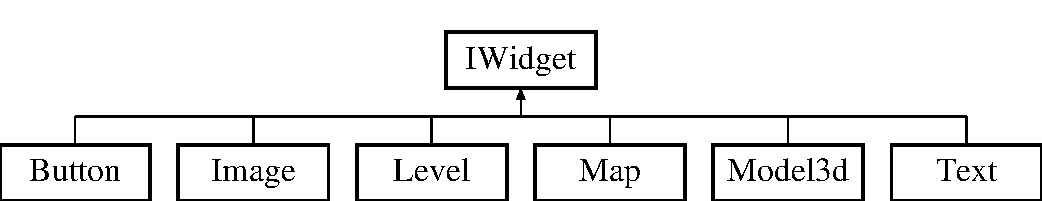
\includegraphics[height=2.000000cm]{classIWidget}
\end{center}
\end{figure}
\subsection*{Public Member Functions}
\begin{DoxyCompactItemize}
\item 
\mbox{\Hypertarget{classIWidget_ad733ed972c58c5c6268b57e2f4381666}\label{classIWidget_ad733ed972c58c5c6268b57e2f4381666}} 
virtual \hyperlink{classIWidget_ad733ed972c58c5c6268b57e2f4381666}{$\sim$\+I\+Widget} ()
\begin{DoxyCompactList}\small\item\em Destructor. \end{DoxyCompactList}\item 
\mbox{\Hypertarget{classIWidget_ad59738ae1350ed490fdbe07cd1ab4daa}\label{classIWidget_ad59738ae1350ed490fdbe07cd1ab4daa}} 
virtual void \hyperlink{classIWidget_ad59738ae1350ed490fdbe07cd1ab4daa}{print} ()=0
\begin{DoxyCompactList}\small\item\em Print the object into the window. \end{DoxyCompactList}\end{DoxyCompactItemize}


\subsection{Detailed Description}
Represent a generic object in the user interface. 

The documentation for this class was generated from the following file\+:\begin{DoxyCompactItemize}
\item 
inc/graphics/widgets/\hyperlink{IWidget_8hh}{I\+Widget.\+hh}\end{DoxyCompactItemize}

\hypertarget{classKeyboard}{}\section{Keyboard Class Reference}
\label{classKeyboard}\index{Keyboard@{Keyboard}}


Handle client keyboard event.  




{\ttfamily \#include $<$Keyboard.\+hh$>$}



Inherits I\+Event\+Receiver.

\subsection*{Public Member Functions}
\begin{DoxyCompactItemize}
\item 
\hyperlink{classKeyboard_abb54d55e7d65dd6ef017352fdf5570c6}{Keyboard} (const irr\+::u32 keyboard\+ID, const irr\+::u32 player\+ID, \hyperlink{structconfig_1_1ControlPlayer}{config\+::\+Control\+Player} control)
\begin{DoxyCompactList}\small\item\em Contructor. \end{DoxyCompactList}\item 
\hyperlink{classKeyboard_af6a99ec66c8c722a45b967bf79167038}{$\sim$\+Keyboard} ()
\begin{DoxyCompactList}\small\item\em Destructor. \end{DoxyCompactList}\item 
virtual bool \hyperlink{classKeyboard_ad6974153a0c29b55c1b8765d0d6ccbfa}{On\+Event} (const irr\+::\+S\+Event \&event)
\begin{DoxyCompactList}\small\item\em On\+Event. \end{DoxyCompactList}\item 
void \hyperlink{classKeyboard_a6c6492921a44b4a4ab7e96566381353c}{notify\+Event\+Manager} (const irr\+::\+S\+Event \&event)
\begin{DoxyCompactList}\small\item\em notify\+Event\+Manager \end{DoxyCompactList}\item 
irr\+::u32 \hyperlink{classKeyboard_ac8fe530866f42dd3a62ea66054bc148b}{get\+Player\+ID} (void) const
\begin{DoxyCompactList}\small\item\em get\+Player\+ID \end{DoxyCompactList}\item 
irr\+::u32 \hyperlink{classKeyboard_a8bc4a7d865e268c0d126aa3f0a913bbb}{get\+Keyboard\+ID} (void) const
\begin{DoxyCompactList}\small\item\em get\+Keyboard\+ID \end{DoxyCompactList}\end{DoxyCompactItemize}


\subsection{Detailed Description}
Handle client keyboard event. 

\subsection{Constructor \& Destructor Documentation}
\mbox{\Hypertarget{classKeyboard_abb54d55e7d65dd6ef017352fdf5570c6}\label{classKeyboard_abb54d55e7d65dd6ef017352fdf5570c6}} 
\index{Keyboard@{Keyboard}!Keyboard@{Keyboard}}
\index{Keyboard@{Keyboard}!Keyboard@{Keyboard}}
\subsubsection{\texorpdfstring{Keyboard()}{Keyboard()}}
{\footnotesize\ttfamily Keyboard\+::\+Keyboard (\begin{DoxyParamCaption}\item[{const irr\+::u32}]{keyboard\+ID,  }\item[{const irr\+::u32}]{player\+ID,  }\item[{\hyperlink{structconfig_1_1ControlPlayer}{config\+::\+Control\+Player}}]{control }\end{DoxyParamCaption})}



Contructor. 

Build the class


\begin{DoxyParams}{Parameters}
{\em keyboard\+ID} & Define the id of keyboard\\
\hline
{\em player\+ID} & Define the id of player\\
\hline
{\em control} & Link the control to the \hyperlink{classKeyboard}{Keyboard} \\
\hline
\end{DoxyParams}
\mbox{\Hypertarget{classKeyboard_af6a99ec66c8c722a45b967bf79167038}\label{classKeyboard_af6a99ec66c8c722a45b967bf79167038}} 
\index{Keyboard@{Keyboard}!````~Keyboard@{$\sim$\+Keyboard}}
\index{````~Keyboard@{$\sim$\+Keyboard}!Keyboard@{Keyboard}}
\subsubsection{\texorpdfstring{$\sim$\+Keyboard()}{~Keyboard()}}
{\footnotesize\ttfamily Keyboard\+::$\sim$\+Keyboard (\begin{DoxyParamCaption}{ }\end{DoxyParamCaption})}



Destructor. 

Destroy the class 

\subsection{Member Function Documentation}
\mbox{\Hypertarget{classKeyboard_a8bc4a7d865e268c0d126aa3f0a913bbb}\label{classKeyboard_a8bc4a7d865e268c0d126aa3f0a913bbb}} 
\index{Keyboard@{Keyboard}!get\+Keyboard\+ID@{get\+Keyboard\+ID}}
\index{get\+Keyboard\+ID@{get\+Keyboard\+ID}!Keyboard@{Keyboard}}
\subsubsection{\texorpdfstring{get\+Keyboard\+I\+D()}{getKeyboardID()}}
{\footnotesize\ttfamily Unsigned\+Int Keyboard\+::get\+Keyboard\+ID (\begin{DoxyParamCaption}\item[{void}]{ }\end{DoxyParamCaption}) const}



get\+Keyboard\+ID 

Return \+\_\+keyboard\+ID \mbox{\Hypertarget{classKeyboard_ac8fe530866f42dd3a62ea66054bc148b}\label{classKeyboard_ac8fe530866f42dd3a62ea66054bc148b}} 
\index{Keyboard@{Keyboard}!get\+Player\+ID@{get\+Player\+ID}}
\index{get\+Player\+ID@{get\+Player\+ID}!Keyboard@{Keyboard}}
\subsubsection{\texorpdfstring{get\+Player\+I\+D()}{getPlayerID()}}
{\footnotesize\ttfamily Unsigned\+Int Keyboard\+::get\+Player\+ID (\begin{DoxyParamCaption}\item[{void}]{ }\end{DoxyParamCaption}) const}



get\+Player\+ID 

Return \+\_\+playeriD \mbox{\Hypertarget{classKeyboard_a6c6492921a44b4a4ab7e96566381353c}\label{classKeyboard_a6c6492921a44b4a4ab7e96566381353c}} 
\index{Keyboard@{Keyboard}!notify\+Event\+Manager@{notify\+Event\+Manager}}
\index{notify\+Event\+Manager@{notify\+Event\+Manager}!Keyboard@{Keyboard}}
\subsubsection{\texorpdfstring{notify\+Event\+Manager()}{notifyEventManager()}}
{\footnotesize\ttfamily void Keyboard\+::notify\+Event\+Manager (\begin{DoxyParamCaption}\item[{const irr\+::\+S\+Event \&}]{event }\end{DoxyParamCaption})}



notify\+Event\+Manager 

Handle the event and send the event in the Queue


\begin{DoxyParams}{Parameters}
{\em event} & event sent by Onevent \\
\hline
\end{DoxyParams}
\mbox{\Hypertarget{classKeyboard_ad6974153a0c29b55c1b8765d0d6ccbfa}\label{classKeyboard_ad6974153a0c29b55c1b8765d0d6ccbfa}} 
\index{Keyboard@{Keyboard}!On\+Event@{On\+Event}}
\index{On\+Event@{On\+Event}!Keyboard@{Keyboard}}
\subsubsection{\texorpdfstring{On\+Event()}{OnEvent()}}
{\footnotesize\ttfamily bool Keyboard\+::\+On\+Event (\begin{DoxyParamCaption}\item[{const irr\+::\+S\+Event \&}]{event }\end{DoxyParamCaption})\hspace{0.3cm}{\ttfamily [virtual]}}



On\+Event. 

Call the notify manager


\begin{DoxyParams}{Parameters}
{\em event} & event sent by irrlicht \\
\hline
\end{DoxyParams}


The documentation for this class was generated from the following files\+:\begin{DoxyCompactItemize}
\item 
inc/event/\hyperlink{Keyboard_8hh}{Keyboard.\+hh}\item 
src/event/Keyboard.\+cpp\end{DoxyCompactItemize}

\hypertarget{classLegendScene}{}\section{Legend\+Scene Class Reference}
\label{classLegendScene}\index{Legend\+Scene@{Legend\+Scene}}


\hyperlink{classButton}{Button} interface of \hyperlink{classLegendScene}{Legend\+Scene}.  




{\ttfamily \#include $<$Legend\+Scene.\+hh$>$}

Inheritance diagram for Legend\+Scene\+:\begin{figure}[H]
\begin{center}
\leavevmode
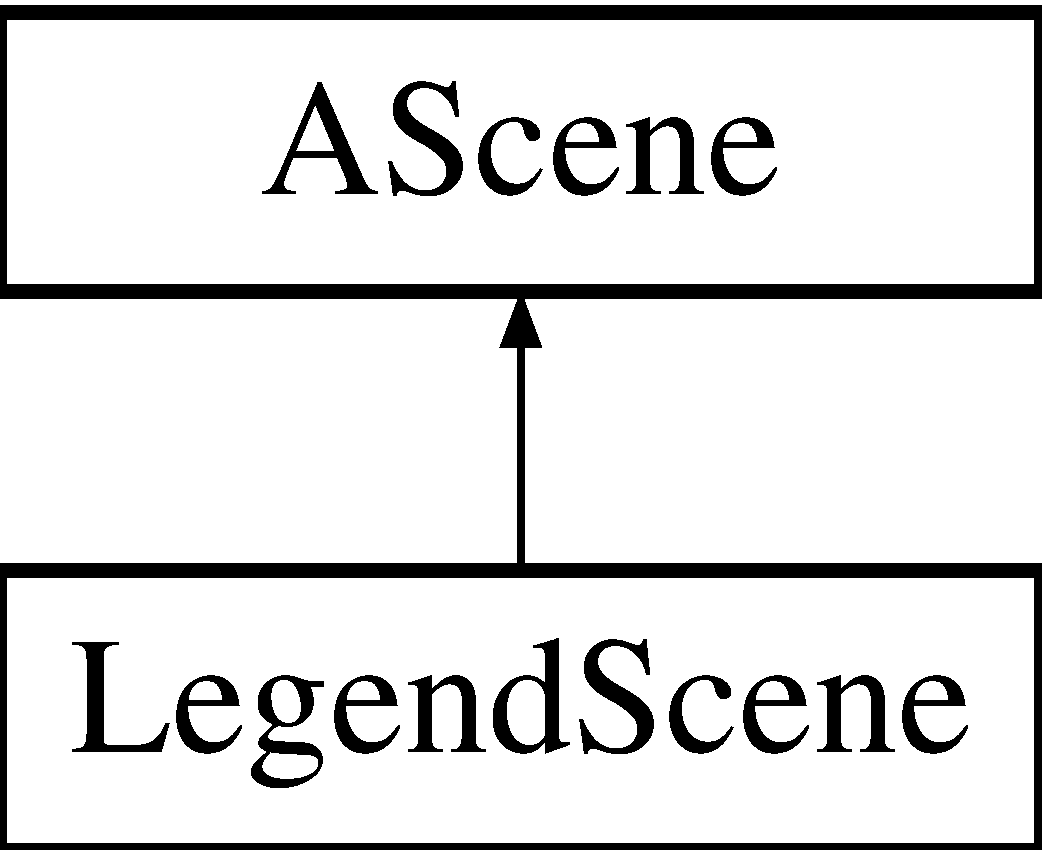
\includegraphics[height=2.000000cm]{classLegendScene}
\end{center}
\end{figure}
\subsection*{Public Member Functions}
\begin{DoxyCompactItemize}
\item 
\hyperlink{classLegendScene_a33a4d96e0e320724e60d565dec448e38}{Legend\+Scene} ()
\begin{DoxyCompactList}\small\item\em Constructor. \end{DoxyCompactList}\item 
\hyperlink{classLegendScene_a88e66f9964236616735c7b9873641141}{$\sim$\+Legend\+Scene} ()
\begin{DoxyCompactList}\small\item\em Destructor. \end{DoxyCompactList}\item 
\hyperlink{classirr_1_1IEventReceiver}{irr\+::\+I\+Event\+Receiver} $\ast$ \hyperlink{classLegendScene_ab11340ae844c04d704f28e1ef188deae}{get\+Event\+Receiver} () const
\begin{DoxyCompactList}\small\item\em Event getter. \end{DoxyCompactList}\end{DoxyCompactItemize}


\subsection{Detailed Description}
\hyperlink{classButton}{Button} interface of \hyperlink{classLegendScene}{Legend\+Scene}. 

\subsection{Constructor \& Destructor Documentation}
\mbox{\Hypertarget{classLegendScene_a33a4d96e0e320724e60d565dec448e38}\label{classLegendScene_a33a4d96e0e320724e60d565dec448e38}} 
\index{Legend\+Scene@{Legend\+Scene}!Legend\+Scene@{Legend\+Scene}}
\index{Legend\+Scene@{Legend\+Scene}!Legend\+Scene@{Legend\+Scene}}
\subsubsection{\texorpdfstring{Legend\+Scene()}{LegendScene()}}
{\footnotesize\ttfamily Legend\+Scene\+::\+Legend\+Scene (\begin{DoxyParamCaption}{ }\end{DoxyParamCaption})}



Constructor. 

Build the class. \mbox{\Hypertarget{classLegendScene_a88e66f9964236616735c7b9873641141}\label{classLegendScene_a88e66f9964236616735c7b9873641141}} 
\index{Legend\+Scene@{Legend\+Scene}!````~Legend\+Scene@{$\sim$\+Legend\+Scene}}
\index{````~Legend\+Scene@{$\sim$\+Legend\+Scene}!Legend\+Scene@{Legend\+Scene}}
\subsubsection{\texorpdfstring{$\sim$\+Legend\+Scene()}{~LegendScene()}}
{\footnotesize\ttfamily Legend\+Scene\+::$\sim$\+Legend\+Scene (\begin{DoxyParamCaption}{ }\end{DoxyParamCaption})}



Destructor. 

Destroy the class. 

\subsection{Member Function Documentation}
\mbox{\Hypertarget{classLegendScene_ab11340ae844c04d704f28e1ef188deae}\label{classLegendScene_ab11340ae844c04d704f28e1ef188deae}} 
\index{Legend\+Scene@{Legend\+Scene}!get\+Event\+Receiver@{get\+Event\+Receiver}}
\index{get\+Event\+Receiver@{get\+Event\+Receiver}!Legend\+Scene@{Legend\+Scene}}
\subsubsection{\texorpdfstring{get\+Event\+Receiver()}{getEventReceiver()}}
{\footnotesize\ttfamily \hyperlink{classirr_1_1IEventReceiver}{irr\+::\+I\+Event\+Receiver} $\ast$ Legend\+Scene\+::get\+Event\+Receiver (\begin{DoxyParamCaption}{ }\end{DoxyParamCaption}) const\hspace{0.3cm}{\ttfamily [virtual]}}



Event getter. 

Return the event. 

Implements \hyperlink{classAScene_af521e5e6d30a5d2e5d30eb333e4d3abd}{A\+Scene}.



The documentation for this class was generated from the following files\+:\begin{DoxyCompactItemize}
\item 
inc/graphics/scenes/\hyperlink{LegendScene_8hh}{Legend\+Scene.\+hh}\item 
src/graphics/scenes/Legend\+Scene.\+cpp\end{DoxyCompactItemize}

\hypertarget{classLevel}{}\section{Level Class Reference}
\label{classLevel}\index{Level@{Level}}


Represent a game\textquotesingle{}s level.  




{\ttfamily \#include $<$Level.\+hh$>$}

Inheritance diagram for Level\+:\begin{figure}[H]
\begin{center}
\leavevmode
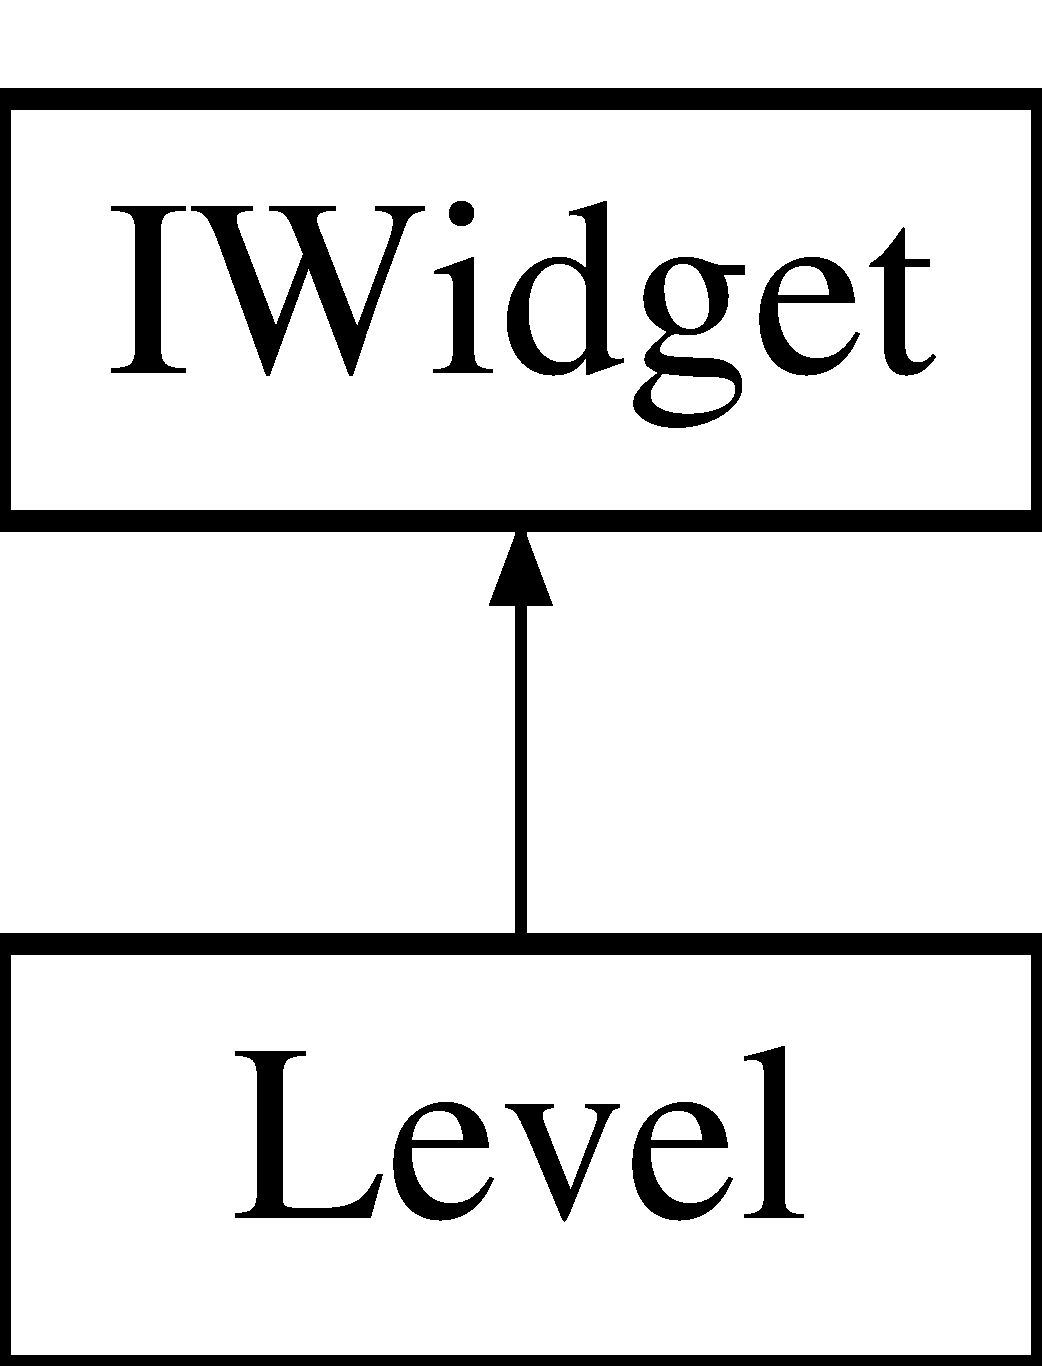
\includegraphics[height=2.000000cm]{classLevel}
\end{center}
\end{figure}
\subsection*{Public Member Functions}
\begin{DoxyCompactItemize}
\item 
\hyperlink{classLevel_a1cddef79da66a80002686199a847543f}{Level} (const W\+String \&map\+Path, std\+::vector$<$ std\+::shared\+\_\+ptr$<$ A\+Hero $>$ $>$ players=std\+::vector$<$ std\+::shared\+\_\+ptr$<$ A\+Hero $>$ $>$(), std\+::vector$<$ std\+::shared\+\_\+ptr$<$ A\+Monster $>$ $>$ monsters=std\+::vector$<$ std\+::shared\+\_\+ptr$<$ A\+Monster $>$ $>$(), std\+::vector$<$ std\+::shared\+\_\+ptr$<$ \hyperlink{classAPickable}{A\+Pickable} $>$ $>$ objects=std\+::vector$<$ std\+::shared\+\_\+ptr$<$ \hyperlink{classAPickable}{A\+Pickable} $>$ $>$())
\begin{DoxyCompactList}\small\item\em Constructor. \end{DoxyCompactList}\item 
\hyperlink{classLevel_a249eac1e8f19ff44134efa5e986feaca}{$\sim$\+Level} ()
\begin{DoxyCompactList}\small\item\em Destructor. \end{DoxyCompactList}\item 
void \hyperlink{classLevel_aa88db36cd824320cb599d913603dc2a3}{load\+Level} ()
\item 
void \hyperlink{classLevel_ab8311fe64b7957d627053359331b0b6b}{print} (\hyperlink{classWindow}{Window} $\ast$win)
\begin{DoxyCompactList}\small\item\em Print the object into the window. \end{DoxyCompactList}\end{DoxyCompactItemize}


\subsection{Detailed Description}
Represent a game\textquotesingle{}s level. 

\subsection{Constructor \& Destructor Documentation}
\mbox{\Hypertarget{classLevel_a1cddef79da66a80002686199a847543f}\label{classLevel_a1cddef79da66a80002686199a847543f}} 
\index{Level@{Level}!Level@{Level}}
\index{Level@{Level}!Level@{Level}}
\subsubsection{\texorpdfstring{Level()}{Level()}}
{\footnotesize\ttfamily Level\+::\+Level (\begin{DoxyParamCaption}\item[{const W\+String \&}]{map\+Path,  }\item[{std\+::vector$<$ std\+::shared\+\_\+ptr$<$ A\+Hero $>$ $>$}]{players = {\ttfamily std\+:\+:vector$<$~std\+:\+:shared\+\_\+ptr$<$AHero$>$~$>$()},  }\item[{std\+::vector$<$ std\+::shared\+\_\+ptr$<$ A\+Monster $>$ $>$}]{monsters = {\ttfamily std\+:\+:vector$<$~std\+:\+:shared\+\_\+ptr$<$AMonster$>$~$>$()},  }\item[{std\+::vector$<$ std\+::shared\+\_\+ptr$<$ \hyperlink{classAPickable}{A\+Pickable} $>$ $>$}]{objects = {\ttfamily std\+:\+:vector$<$~std\+:\+:shared\+\_\+ptr$<$\hyperlink{classAPickable}{A\+Pickable}$>$~$>$()} }\end{DoxyParamCaption})}



Constructor. 

Build the class \mbox{\Hypertarget{classLevel_a249eac1e8f19ff44134efa5e986feaca}\label{classLevel_a249eac1e8f19ff44134efa5e986feaca}} 
\index{Level@{Level}!````~Level@{$\sim$\+Level}}
\index{````~Level@{$\sim$\+Level}!Level@{Level}}
\subsubsection{\texorpdfstring{$\sim$\+Level()}{~Level()}}
{\footnotesize\ttfamily Level\+::$\sim$\+Level (\begin{DoxyParamCaption}{ }\end{DoxyParamCaption})}



Destructor. 

Destroy the class 

\subsection{Member Function Documentation}
\mbox{\Hypertarget{classLevel_aa88db36cd824320cb599d913603dc2a3}\label{classLevel_aa88db36cd824320cb599d913603dc2a3}} 
\index{Level@{Level}!load\+Level@{load\+Level}}
\index{load\+Level@{load\+Level}!Level@{Level}}
\subsubsection{\texorpdfstring{load\+Level()}{loadLevel()}}
{\footnotesize\ttfamily void Level\+::load\+Level (\begin{DoxyParamCaption}{ }\end{DoxyParamCaption})}

load level according to X\+ML file xml is loaded thankfully to level\+Number Loading \+:
\begin{DoxyItemize}
\item map
\item player
\item monsters
\item pickable objects 
\end{DoxyItemize}\mbox{\Hypertarget{classLevel_ab8311fe64b7957d627053359331b0b6b}\label{classLevel_ab8311fe64b7957d627053359331b0b6b}} 
\index{Level@{Level}!print@{print}}
\index{print@{print}!Level@{Level}}
\subsubsection{\texorpdfstring{print()}{print()}}
{\footnotesize\ttfamily void Level\+::print (\begin{DoxyParamCaption}\item[{\hyperlink{classWindow}{Window} $\ast$}]{win }\end{DoxyParamCaption})\hspace{0.3cm}{\ttfamily [virtual]}}



Print the object into the window. 


\begin{DoxyParams}{Parameters}
{\em \textquotesingle{}window\textquotesingle{}} & the window where the object will be print. \\
\hline
\end{DoxyParams}
T\+O\+DO Print player Print monsters Print pickable objects

Implements \hyperlink{classIWidget_a0cfa49a402e9bb31808a715e048ab2f4}{I\+Widget}.



The documentation for this class was generated from the following files\+:\begin{DoxyCompactItemize}
\item 
inc/game/level/\hyperlink{Level_8hh}{Level.\+hh}\item 
src/game/level/Level.\+cpp\end{DoxyCompactItemize}

\hypertarget{classMainScene}{}\section{Main\+Scene Class Reference}
\label{classMainScene}\index{Main\+Scene@{Main\+Scene}}


\hyperlink{classButton}{Button} interface of main scene.  




{\ttfamily \#include $<$Main\+Scene.\+hh$>$}

Inheritance diagram for Main\+Scene\+:\begin{figure}[H]
\begin{center}
\leavevmode
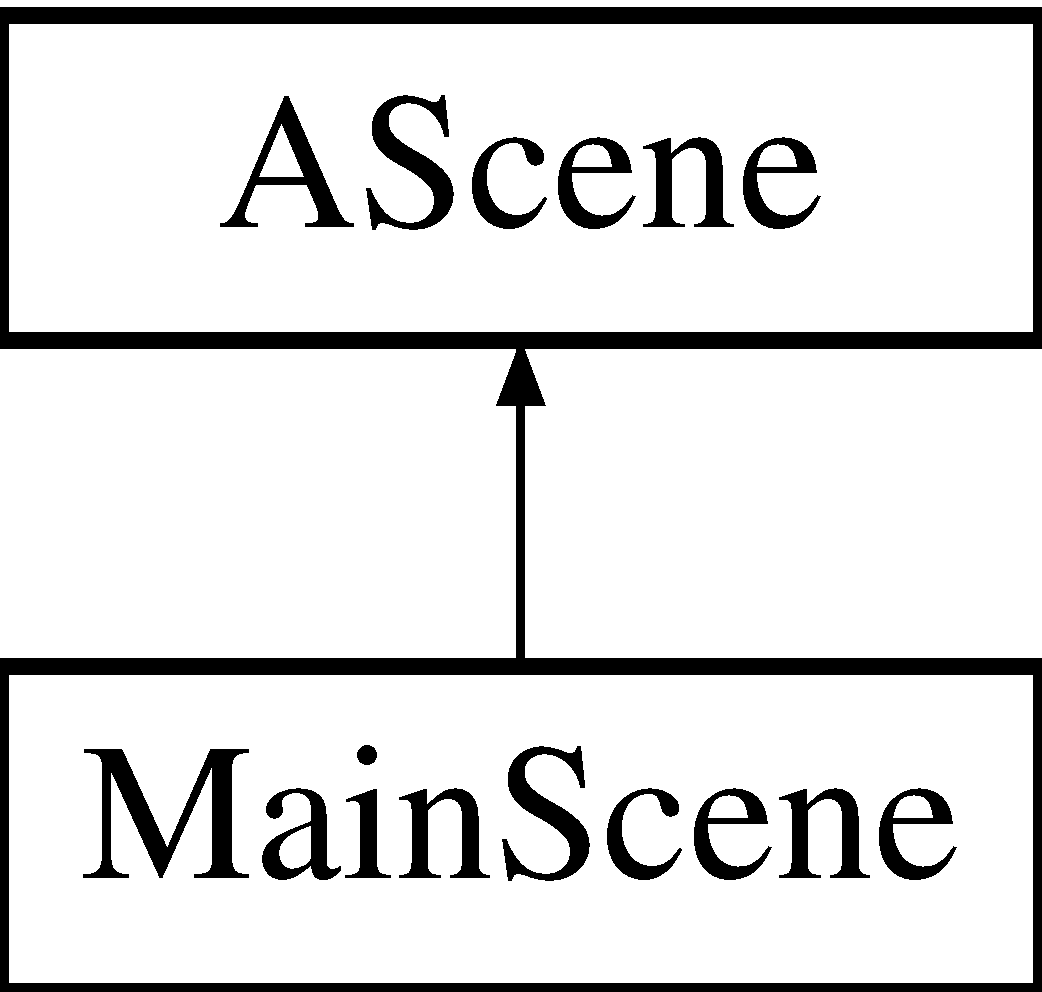
\includegraphics[height=2.000000cm]{classMainScene}
\end{center}
\end{figure}
\subsection*{Public Member Functions}
\begin{DoxyCompactItemize}
\item 
\hyperlink{classMainScene_ad0d02863b2e1eaf96d4d2f9277398afc}{Main\+Scene} ()
\begin{DoxyCompactList}\small\item\em Constructor. \end{DoxyCompactList}\item 
\hyperlink{classMainScene_a6f5a9b6606eb0534d828a11881e0a73f}{$\sim$\+Main\+Scene} ()
\begin{DoxyCompactList}\small\item\em Destructor. \end{DoxyCompactList}\item 
\hyperlink{classirr_1_1IEventReceiver}{irr\+::\+I\+Event\+Receiver} $\ast$ \hyperlink{classMainScene_af9fbc6337aa6ff42447c702e91e77237}{get\+Event\+Receiver} () const
\begin{DoxyCompactList}\small\item\em Event getter. \end{DoxyCompactList}\end{DoxyCompactItemize}


\subsection{Detailed Description}
\hyperlink{classButton}{Button} interface of main scene. 

\subsection{Constructor \& Destructor Documentation}
\mbox{\Hypertarget{classMainScene_ad0d02863b2e1eaf96d4d2f9277398afc}\label{classMainScene_ad0d02863b2e1eaf96d4d2f9277398afc}} 
\index{Main\+Scene@{Main\+Scene}!Main\+Scene@{Main\+Scene}}
\index{Main\+Scene@{Main\+Scene}!Main\+Scene@{Main\+Scene}}
\subsubsection{\texorpdfstring{Main\+Scene()}{MainScene()}}
{\footnotesize\ttfamily Main\+Scene\+::\+Main\+Scene (\begin{DoxyParamCaption}{ }\end{DoxyParamCaption})}



Constructor. 

Build the class. \mbox{\Hypertarget{classMainScene_a6f5a9b6606eb0534d828a11881e0a73f}\label{classMainScene_a6f5a9b6606eb0534d828a11881e0a73f}} 
\index{Main\+Scene@{Main\+Scene}!````~Main\+Scene@{$\sim$\+Main\+Scene}}
\index{````~Main\+Scene@{$\sim$\+Main\+Scene}!Main\+Scene@{Main\+Scene}}
\subsubsection{\texorpdfstring{$\sim$\+Main\+Scene()}{~MainScene()}}
{\footnotesize\ttfamily Main\+Scene\+::$\sim$\+Main\+Scene (\begin{DoxyParamCaption}{ }\end{DoxyParamCaption})}



Destructor. 

Destroy the class. 

\subsection{Member Function Documentation}
\mbox{\Hypertarget{classMainScene_af9fbc6337aa6ff42447c702e91e77237}\label{classMainScene_af9fbc6337aa6ff42447c702e91e77237}} 
\index{Main\+Scene@{Main\+Scene}!get\+Event\+Receiver@{get\+Event\+Receiver}}
\index{get\+Event\+Receiver@{get\+Event\+Receiver}!Main\+Scene@{Main\+Scene}}
\subsubsection{\texorpdfstring{get\+Event\+Receiver()}{getEventReceiver()}}
{\footnotesize\ttfamily \hyperlink{classirr_1_1IEventReceiver}{irr\+::\+I\+Event\+Receiver} $\ast$ Main\+Scene\+::get\+Event\+Receiver (\begin{DoxyParamCaption}{ }\end{DoxyParamCaption}) const\hspace{0.3cm}{\ttfamily [virtual]}}



Event getter. 

Return the event. 

Implements \hyperlink{classAScene_af521e5e6d30a5d2e5d30eb333e4d3abd}{A\+Scene}.



The documentation for this class was generated from the following files\+:\begin{DoxyCompactItemize}
\item 
inc/graphics/scenes/\hyperlink{MainScene_8hh}{Main\+Scene.\+hh}\item 
src/graphics/scenes/Main\+Scene.\+cpp\end{DoxyCompactItemize}

\hypertarget{classMap}{}\section{Map Class Reference}
\label{classMap}\index{Map@{Map}}


Represent a level\textquotesingle{}s map.  




{\ttfamily \#include $<$Map.\+hh$>$}

Inheritance diagram for Map\+:\begin{figure}[H]
\begin{center}
\leavevmode
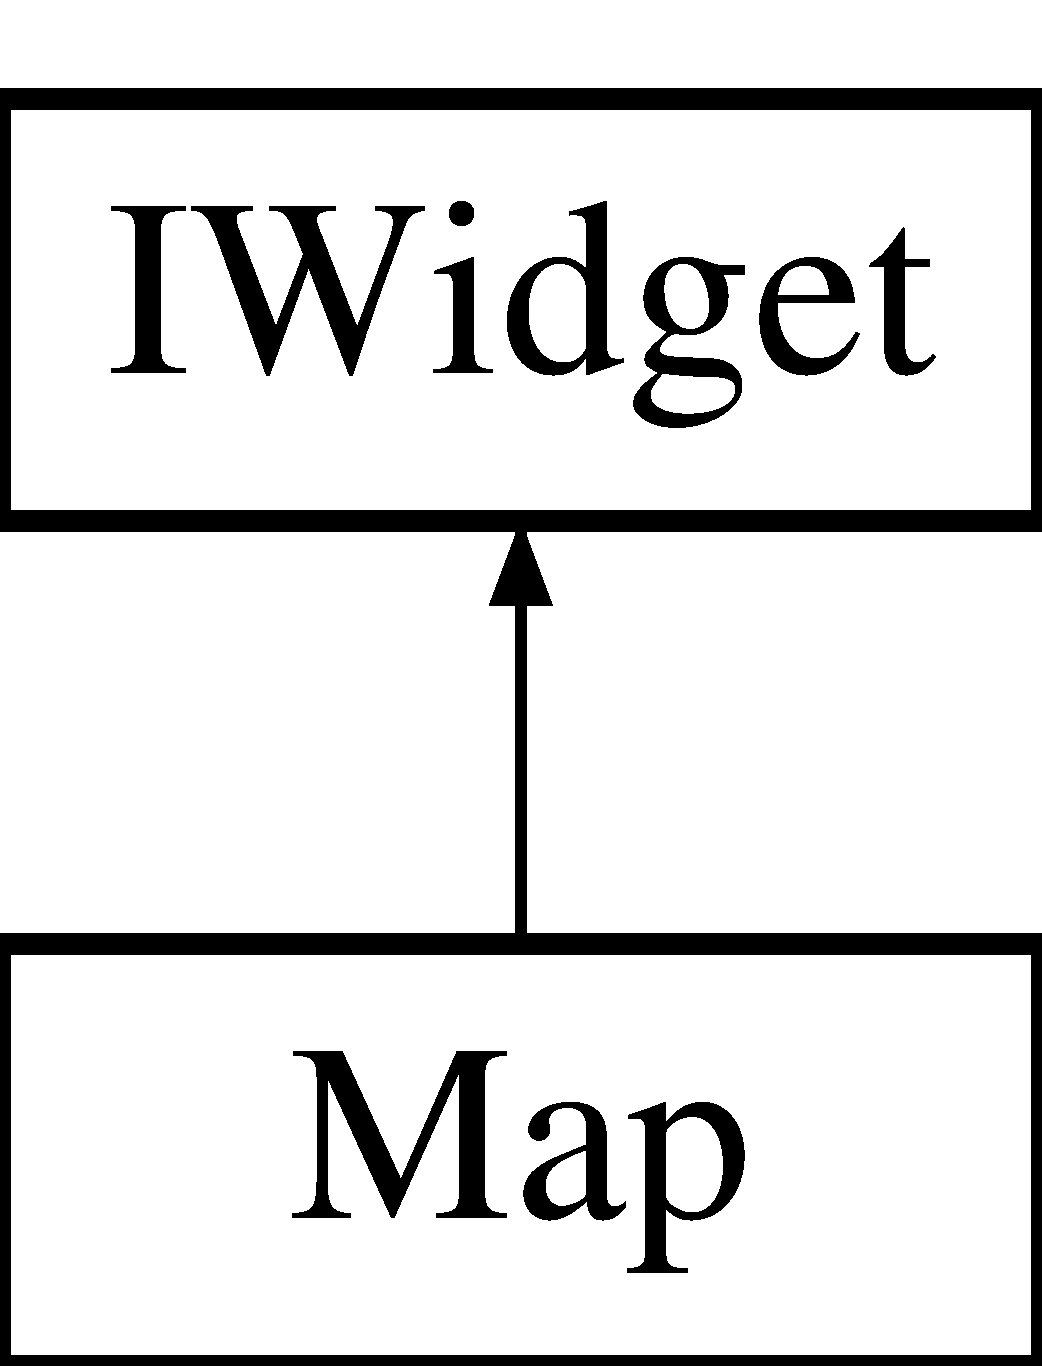
\includegraphics[height=2.000000cm]{classMap}
\end{center}
\end{figure}
\subsection*{Public Member Functions}
\begin{DoxyCompactItemize}
\item 
\hyperlink{classMap_a2e6d2bce865999917deae256baaa434d}{Map} (W\+String const map\+Name)
\begin{DoxyCompactList}\small\item\em Constructs the map with the related file. \end{DoxyCompactList}\item 
\mbox{\Hypertarget{classMap_aa403fbe09394ccf39747588f5168e3b2}\label{classMap_aa403fbe09394ccf39747588f5168e3b2}} 
\hyperlink{classMap_aa403fbe09394ccf39747588f5168e3b2}{$\sim$\+Map} ()
\begin{DoxyCompactList}\small\item\em Destructor... \end{DoxyCompactList}\item 
\mbox{\Hypertarget{classMap_a9c6dc88a70dcf25e3371d8bc4ec35ad0}\label{classMap_a9c6dc88a70dcf25e3371d8bc4ec35ad0}} 
void \hyperlink{classMap_a9c6dc88a70dcf25e3371d8bc4ec35ad0}{print} ()
\begin{DoxyCompactList}\small\item\em Print the map into the window, by adding some nodes into the scene manager. \end{DoxyCompactList}\item 
\mbox{\Hypertarget{classMap_a47f72d481d0ed624dfd03e63ebd281e5}\label{classMap_a47f72d481d0ed624dfd03e63ebd281e5}} 
W\+String const \hyperlink{classMap_a47f72d481d0ed624dfd03e63ebd281e5}{get\+Map\+Path} (void) const
\begin{DoxyCompactList}\small\item\em Accessor on map name. \end{DoxyCompactList}\item 
bool \hyperlink{classMap_ae085956bff7ba817bb82fc37bb8231df}{load\+Map} () const
\begin{DoxyCompactList}\small\item\em Load map in global scene manager. \end{DoxyCompactList}\item 
bool \hyperlink{classMap_a7b66b582699a4ea8108eebd86b1aca57}{load\+Scene\+Nodes} ()
\begin{DoxyCompactList}\small\item\em Load all the nodes of the map. \end{DoxyCompactList}\item 
\mbox{\Hypertarget{classMap_af7e0fd073da4026f58370b0e5f207e9d}\label{classMap_af7e0fd073da4026f58370b0e5f207e9d}} 
bool \hyperlink{classMap_af7e0fd073da4026f58370b0e5f207e9d}{init\+Collision\+Response\+Animator} ()
\begin{DoxyCompactList}\small\item\em Initialize the collisions. \end{DoxyCompactList}\end{DoxyCompactItemize}


\subsection{Detailed Description}
Represent a level\textquotesingle{}s map. 

\subsection{Constructor \& Destructor Documentation}
\mbox{\Hypertarget{classMap_a2e6d2bce865999917deae256baaa434d}\label{classMap_a2e6d2bce865999917deae256baaa434d}} 
\index{Map@{Map}!Map@{Map}}
\index{Map@{Map}!Map@{Map}}
\subsubsection{\texorpdfstring{Map()}{Map()}}
{\footnotesize\ttfamily Map\+::\+Map (\begin{DoxyParamCaption}\item[{W\+String const}]{map\+Name }\end{DoxyParamCaption})}



Constructs the map with the related file. 


\begin{DoxyParams}{Parameters}
{\em map\+Name} & \+: the related .irr map file \\
\hline
\end{DoxyParams}


\subsection{Member Function Documentation}
\mbox{\Hypertarget{classMap_ae085956bff7ba817bb82fc37bb8231df}\label{classMap_ae085956bff7ba817bb82fc37bb8231df}} 
\index{Map@{Map}!load\+Map@{load\+Map}}
\index{load\+Map@{load\+Map}!Map@{Map}}
\subsubsection{\texorpdfstring{load\+Map()}{loadMap()}}
{\footnotesize\ttfamily bool Map\+::load\+Map (\begin{DoxyParamCaption}{ }\end{DoxyParamCaption}) const}



Load map in global scene manager. 

.irr files can store the whole scene graph including animators, materials and particle systems. And there is also the possibility to store arbitrary user data for every scene node in that file. this example simple, we are simply loading the scene here. See the documentation at I\+Scene\+Manager\+::load\+Scene and I\+Scene\+Manager\+::save\+Scene for more information. \mbox{\Hypertarget{classMap_a7b66b582699a4ea8108eebd86b1aca57}\label{classMap_a7b66b582699a4ea8108eebd86b1aca57}} 
\index{Map@{Map}!load\+Scene\+Nodes@{load\+Scene\+Nodes}}
\index{load\+Scene\+Nodes@{load\+Scene\+Nodes}!Map@{Map}}
\subsubsection{\texorpdfstring{load\+Scene\+Nodes()}{loadSceneNodes()}}
{\footnotesize\ttfamily bool Map\+::load\+Scene\+Nodes (\begin{DoxyParamCaption}{ }\end{DoxyParamCaption})}



Load all the nodes of the map. 

We find all the nodes in the scene It would be possible to make a more informed decision about which nodes to perform collision checks on. We would such capture that information in the node name/id. 

The documentation for this class was generated from the following files\+:\begin{DoxyCompactItemize}
\item 
inc/game/level/\hyperlink{Map_8hh}{Map.\+hh}\item 
src/game/level/Map.\+cpp\end{DoxyCompactItemize}

\hypertarget{classMapFactory}{}\section{Map\+Factory Class Reference}
\label{classMapFactory}\index{Map\+Factory@{Map\+Factory}}


Represent a maps\textquotesingle{} factory.  




{\ttfamily \#include $<$Map\+Factory.\+hh$>$}



\subsection{Detailed Description}
Represent a maps\textquotesingle{} factory. 

The documentation for this class was generated from the following files\+:\begin{DoxyCompactItemize}
\item 
inc/game/level/\hyperlink{MapFactory_8hh}{Map\+Factory.\+hh}\item 
src/game/level/Map\+Factory.\+cpp\end{DoxyCompactItemize}

\hypertarget{classModel3d}{}\section{Model3d Class Reference}
\label{classModel3d}\index{Model3d@{Model3d}}


Represent a model 3d in the user interface.  




{\ttfamily \#include $<$Model3d.\+hh$>$}

Inheritance diagram for Model3d\+:\begin{figure}[H]
\begin{center}
\leavevmode
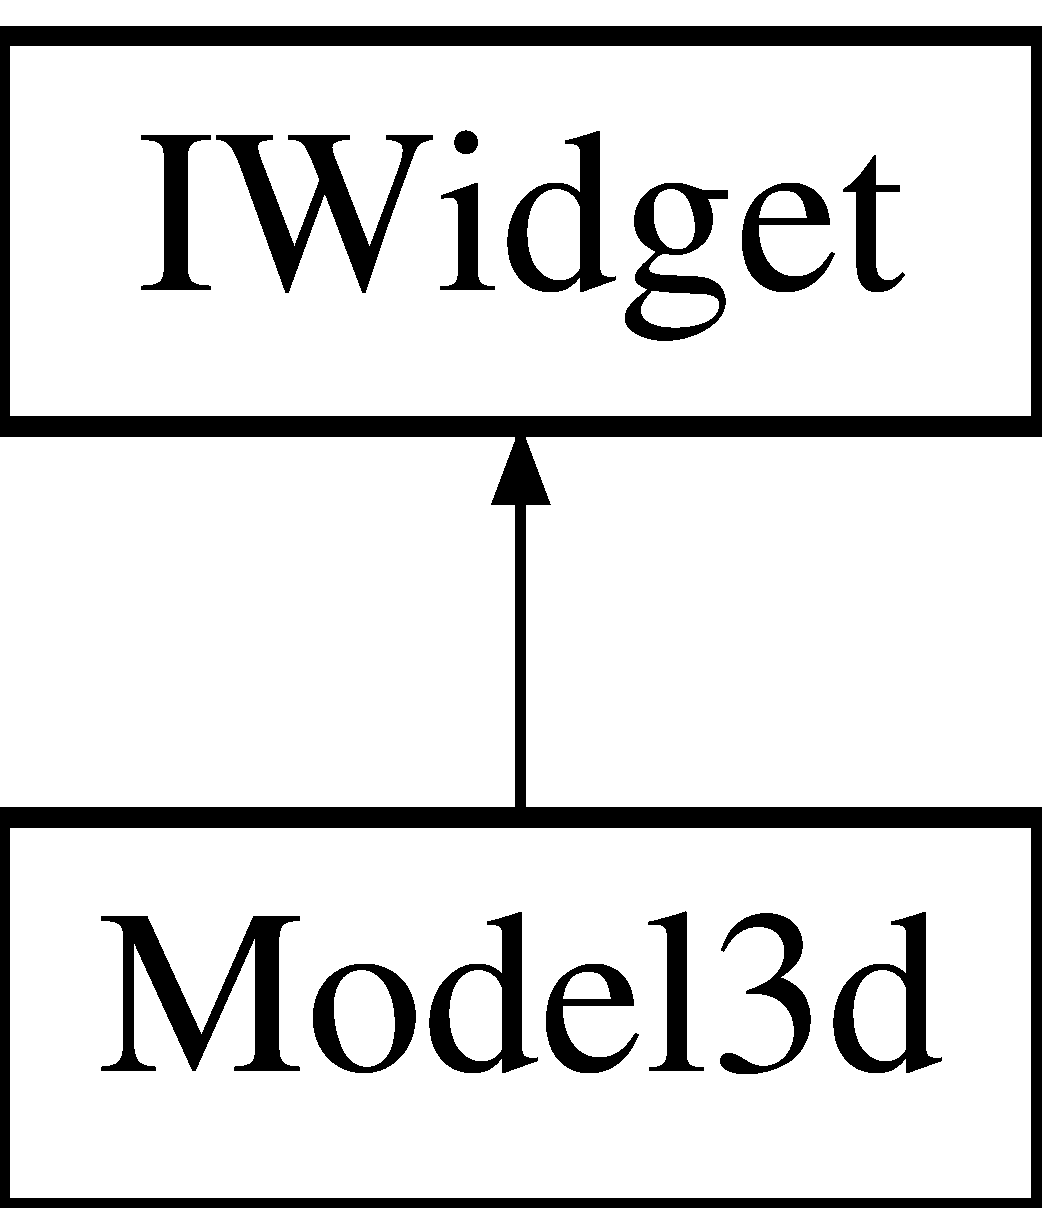
\includegraphics[height=2.000000cm]{classModel3d}
\end{center}
\end{figure}
\subsection*{Classes}
\begin{DoxyCompactItemize}
\item 
struct \hyperlink{structModel3d_1_1Animation}{Animation}
\begin{DoxyCompactList}\small\item\em Represent a model\textquotesingle{}s animation. \end{DoxyCompactList}\item 
struct \hyperlink{structModel3d_1_1AnimationSetting}{Animation\+Setting}
\begin{DoxyCompactList}\small\item\em Represent a model\textquotesingle{}s animation\textquotesingle{}s setting. \end{DoxyCompactList}\end{DoxyCompactItemize}
\subsection*{Public Member Functions}
\begin{DoxyCompactItemize}
\item 
\hyperlink{classModel3d_a3382c1519f85b695a1d98b492207c339}{Model3d} (const String \&file\+X\+ML, const Vector3d \&position, const Vector3d \&rotation, Float scale=1, size\+\_\+t animation\+Speed=4)
\begin{DoxyCompactList}\small\item\em Constructor. \end{DoxyCompactList}\item 
\mbox{\Hypertarget{classModel3d_a7a4ec3be34c901538574d99d95a46b04}\label{classModel3d_a7a4ec3be34c901538574d99d95a46b04}} 
\hyperlink{classModel3d_a7a4ec3be34c901538574d99d95a46b04}{$\sim$\+Model3d} ()
\begin{DoxyCompactList}\small\item\em Destructor. \end{DoxyCompactList}\item 
\mbox{\Hypertarget{classModel3d_ab1d6c9347c05323f85e5decb7e73cd1e}\label{classModel3d_ab1d6c9347c05323f85e5decb7e73cd1e}} 
void \hyperlink{classModel3d_ab1d6c9347c05323f85e5decb7e73cd1e}{print} ()
\begin{DoxyCompactList}\small\item\em Print the model 3d into the window. \end{DoxyCompactList}\item 
void \hyperlink{classModel3d_a29eeaa6769b0c21268f4704ac2d404b7}{set\+Current\+Anim} (const String \&name)
\begin{DoxyCompactList}\small\item\em Allow to change the current animated mesh of the model. \end{DoxyCompactList}\item 
void \hyperlink{classModel3d_a971b77ce978903443e71187ceafa1528}{set\+Position} (const Vector3d \&pos)
\begin{DoxyCompactList}\small\item\em Set the model\textquotesingle{}s position. \end{DoxyCompactList}\item 
\mbox{\Hypertarget{classModel3d_ac40de3ff1527b92c7eadc80766c87824}\label{classModel3d_ac40de3ff1527b92c7eadc80766c87824}} 
Vector3d \hyperlink{classModel3d_ac40de3ff1527b92c7eadc80766c87824}{get\+Position} (void) const
\begin{DoxyCompactList}\small\item\em Get the model\textquotesingle{}s position. \end{DoxyCompactList}\item 
\mbox{\Hypertarget{classModel3d_a10401849cf36b84946774602e73c7ac9}\label{classModel3d_a10401849cf36b84946774602e73c7ac9}} 
Vector3d \hyperlink{classModel3d_a10401849cf36b84946774602e73c7ac9}{get\+Rotation} (void) const
\begin{DoxyCompactList}\small\item\em Get the model\textquotesingle{}s rotation. \end{DoxyCompactList}\item 
void \hyperlink{classModel3d_adc3c185a679687b4bf483f89eb2c20a9}{set\+Rotation} (const Vector3d \&rot)
\begin{DoxyCompactList}\small\item\em Set the model\textquotesingle{}s position. \end{DoxyCompactList}\item 
void \hyperlink{classModel3d_a108ab9c13b7ae24cc1711c2e97fbc625}{play\+Animation} (const std\+::shared\+\_\+ptr$<$ \hyperlink{structModel3d_1_1Animation}{Animation} $>$ \&anim)
\begin{DoxyCompactList}\small\item\em Play the annimation. \end{DoxyCompactList}\item 
void \hyperlink{classModel3d_a6ce79286c43bd4a6852c544bdad8ee18}{play\+Animation\+Sound} (const std\+::string \&sound)
\begin{DoxyCompactList}\small\item\em Play the annimation\textquotesingle{}s sound. \end{DoxyCompactList}\item 
\mbox{\Hypertarget{classModel3d_a39fb00dd1aa3bcf6161fb0b1218ec200}\label{classModel3d_a39fb00dd1aa3bcf6161fb0b1218ec200}} 
std\+::size\+\_\+t \hyperlink{classModel3d_a39fb00dd1aa3bcf6161fb0b1218ec200}{get\+Animation\+Speed} () const
\begin{DoxyCompactList}\small\item\em Return the model\textquotesingle{}s animation\textquotesingle{}s speed. \end{DoxyCompactList}\item 
\mbox{\Hypertarget{classModel3d_ac3acf0ae583c5ea4b900c291ef95b9af}\label{classModel3d_ac3acf0ae583c5ea4b900c291ef95b9af}} 
Float \hyperlink{classModel3d_ac3acf0ae583c5ea4b900c291ef95b9af}{get\+Scale} () const
\begin{DoxyCompactList}\small\item\em Return the model\textquotesingle{}s scale. \end{DoxyCompactList}\item 
\mbox{\Hypertarget{classModel3d_afa0ccf1c5b0c571afcfbef4a894e6b3a}\label{classModel3d_afa0ccf1c5b0c571afcfbef4a894e6b3a}} 
String \hyperlink{classModel3d_afa0ccf1c5b0c571afcfbef4a894e6b3a}{get\+Name} () const
\begin{DoxyCompactList}\small\item\em Return the model\textquotesingle{}s name. \end{DoxyCompactList}\end{DoxyCompactItemize}


\subsection{Detailed Description}
Represent a model 3d in the user interface. 

\subsection{Constructor \& Destructor Documentation}
\mbox{\Hypertarget{classModel3d_a3382c1519f85b695a1d98b492207c339}\label{classModel3d_a3382c1519f85b695a1d98b492207c339}} 
\index{Model3d@{Model3d}!Model3d@{Model3d}}
\index{Model3d@{Model3d}!Model3d@{Model3d}}
\subsubsection{\texorpdfstring{Model3d()}{Model3d()}}
{\footnotesize\ttfamily Model3d\+::\+Model3d (\begin{DoxyParamCaption}\item[{const String \&}]{file\+X\+ML,  }\item[{const Vector3d \&}]{position,  }\item[{const Vector3d \&}]{rotation,  }\item[{Float}]{scale = {\ttfamily 1},  }\item[{size\+\_\+t}]{animation\+Speed = {\ttfamily 4} }\end{DoxyParamCaption})}



Constructor. 


\begin{DoxyParams}{Parameters}
{\em file\+X\+ML} & Path to the xml file who describe the model. \\
\hline
{\em position} & The position in the space where the model will be print. \\
\hline
{\em rotation} & The rotation of the model in the space. \\
\hline
{\em scale} & An additionnal scale coefficient for the model. \\
\hline
{\em animation\+Speed} & \hyperlink{structModel3d_1_1Animation}{Animation} speed \\
\hline
\end{DoxyParams}


\subsection{Member Function Documentation}
\mbox{\Hypertarget{classModel3d_a108ab9c13b7ae24cc1711c2e97fbc625}\label{classModel3d_a108ab9c13b7ae24cc1711c2e97fbc625}} 
\index{Model3d@{Model3d}!play\+Animation@{play\+Animation}}
\index{play\+Animation@{play\+Animation}!Model3d@{Model3d}}
\subsubsection{\texorpdfstring{play\+Animation()}{playAnimation()}}
{\footnotesize\ttfamily void Model3d\+::play\+Animation (\begin{DoxyParamCaption}\item[{const std\+::shared\+\_\+ptr$<$ \hyperlink{structModel3d_1_1Animation}{Animation} $>$ \&}]{anim }\end{DoxyParamCaption})}



Play the annimation. 


\begin{DoxyParams}{Parameters}
{\em anim} & The animation to play. \\
\hline
\end{DoxyParams}
\mbox{\Hypertarget{classModel3d_a6ce79286c43bd4a6852c544bdad8ee18}\label{classModel3d_a6ce79286c43bd4a6852c544bdad8ee18}} 
\index{Model3d@{Model3d}!play\+Animation\+Sound@{play\+Animation\+Sound}}
\index{play\+Animation\+Sound@{play\+Animation\+Sound}!Model3d@{Model3d}}
\subsubsection{\texorpdfstring{play\+Animation\+Sound()}{playAnimationSound()}}
{\footnotesize\ttfamily void Model3d\+::play\+Animation\+Sound (\begin{DoxyParamCaption}\item[{const std\+::string \&}]{sound }\end{DoxyParamCaption})}



Play the annimation\textquotesingle{}s sound. 


\begin{DoxyParams}{Parameters}
{\em sound} & The sound\textquotesingle{}s name. \\
\hline
\end{DoxyParams}
\mbox{\Hypertarget{classModel3d_a29eeaa6769b0c21268f4704ac2d404b7}\label{classModel3d_a29eeaa6769b0c21268f4704ac2d404b7}} 
\index{Model3d@{Model3d}!set\+Current\+Anim@{set\+Current\+Anim}}
\index{set\+Current\+Anim@{set\+Current\+Anim}!Model3d@{Model3d}}
\subsubsection{\texorpdfstring{set\+Current\+Anim()}{setCurrentAnim()}}
{\footnotesize\ttfamily void Model3d\+::set\+Current\+Anim (\begin{DoxyParamCaption}\item[{const String \&}]{name }\end{DoxyParamCaption})}



Allow to change the current animated mesh of the model. 


\begin{DoxyParams}{Parameters}
{\em name} & Name of the animation that will be load. \\
\hline
\end{DoxyParams}
\mbox{\Hypertarget{classModel3d_a971b77ce978903443e71187ceafa1528}\label{classModel3d_a971b77ce978903443e71187ceafa1528}} 
\index{Model3d@{Model3d}!set\+Position@{set\+Position}}
\index{set\+Position@{set\+Position}!Model3d@{Model3d}}
\subsubsection{\texorpdfstring{set\+Position()}{setPosition()}}
{\footnotesize\ttfamily void Model3d\+::set\+Position (\begin{DoxyParamCaption}\item[{const Vector3d \&}]{pos }\end{DoxyParamCaption})}



Set the model\textquotesingle{}s position. 


\begin{DoxyParams}{Parameters}
{\em pos} & The position to set. \\
\hline
\end{DoxyParams}
\mbox{\Hypertarget{classModel3d_adc3c185a679687b4bf483f89eb2c20a9}\label{classModel3d_adc3c185a679687b4bf483f89eb2c20a9}} 
\index{Model3d@{Model3d}!set\+Rotation@{set\+Rotation}}
\index{set\+Rotation@{set\+Rotation}!Model3d@{Model3d}}
\subsubsection{\texorpdfstring{set\+Rotation()}{setRotation()}}
{\footnotesize\ttfamily void Model3d\+::set\+Rotation (\begin{DoxyParamCaption}\item[{const Vector3d \&}]{rot }\end{DoxyParamCaption})}



Set the model\textquotesingle{}s position. 


\begin{DoxyParams}{Parameters}
{\em rot} & The rotation to set. \\
\hline
\end{DoxyParams}


The documentation for this class was generated from the following files\+:\begin{DoxyCompactItemize}
\item 
inc/graphics/widgets/\hyperlink{Model3d_8hh}{Model3d.\+hh}\item 
src/graphics/widgets/Model3d.\+cpp\end{DoxyCompactItemize}

\hypertarget{classModelsManager}{}\section{Models\+Manager Class Reference}
\label{classModelsManager}\index{Models\+Manager@{Models\+Manager}}


The class to load all the information about a model.  




{\ttfamily \#include $<$Models\+Manager.\+hh$>$}

\subsection*{Public Member Functions}
\begin{DoxyCompactItemize}
\item 
\mbox{\Hypertarget{classModelsManager_a48f911933ce0a38aa78667e34e8098f4}\label{classModelsManager_a48f911933ce0a38aa78667e34e8098f4}} 
\hyperlink{classModelsManager_a48f911933ce0a38aa78667e34e8098f4}{Models\+Manager} ()
\begin{DoxyCompactList}\small\item\em Constructor. \end{DoxyCompactList}\item 
bool \hyperlink{classModelsManager_a54ac507f91b38c8270f96bca6c639846}{load\+Model} (String path, String model\+Name)
\begin{DoxyCompactList}\small\item\em Allow you to load a model. \end{DoxyCompactList}\item 
const config\+::\+Model $\ast$ \hyperlink{classModelsManager_a8fe0ee355c02692c538c7bae747b55a5}{get\+Model} (String to\+Find) const
\begin{DoxyCompactList}\small\item\em Give you a pointeur to an object Model. \end{DoxyCompactList}\end{DoxyCompactItemize}


\subsection{Detailed Description}
The class to load all the information about a model. 

\subsection{Member Function Documentation}
\mbox{\Hypertarget{classModelsManager_a8fe0ee355c02692c538c7bae747b55a5}\label{classModelsManager_a8fe0ee355c02692c538c7bae747b55a5}} 
\index{Models\+Manager@{Models\+Manager}!get\+Model@{get\+Model}}
\index{get\+Model@{get\+Model}!Models\+Manager@{Models\+Manager}}
\subsubsection{\texorpdfstring{get\+Model()}{getModel()}}
{\footnotesize\ttfamily const config\+::\+Model $\ast$ Models\+Manager\+::get\+Model (\begin{DoxyParamCaption}\item[{String}]{to\+Find }\end{DoxyParamCaption}) const}



Give you a pointeur to an object Model. 


\begin{DoxyParams}{Parameters}
{\em to\+Find} & The name previously given to the model \\
\hline
\end{DoxyParams}
\begin{DoxyReturn}{Returns}
A pointer to the model 
\end{DoxyReturn}
\mbox{\Hypertarget{classModelsManager_a54ac507f91b38c8270f96bca6c639846}\label{classModelsManager_a54ac507f91b38c8270f96bca6c639846}} 
\index{Models\+Manager@{Models\+Manager}!load\+Model@{load\+Model}}
\index{load\+Model@{load\+Model}!Models\+Manager@{Models\+Manager}}
\subsubsection{\texorpdfstring{load\+Model()}{loadModel()}}
{\footnotesize\ttfamily bool Models\+Manager\+::load\+Model (\begin{DoxyParamCaption}\item[{String}]{path,  }\item[{String}]{model\+Name }\end{DoxyParamCaption})}



Allow you to load a model. 


\begin{DoxyParams}{Parameters}
{\em path} & Model path \\
\hline
{\em model\+Name} & Name of the model \\
\hline
\end{DoxyParams}
\begin{DoxyReturn}{Returns}
true is the model is load and false otherwise 
\end{DoxyReturn}


The documentation for this class was generated from the following files\+:\begin{DoxyCompactItemize}
\item 
inc/managers/\hyperlink{ModelsManager_8hh}{Models\+Manager.\+hh}\item 
src/managers/Models\+Manager.\+cpp\end{DoxyCompactItemize}

\hypertarget{classOptionControl}{}\section{Option\+Control Class Reference}
\label{classOptionControl}\index{Option\+Control@{Option\+Control}}


\hyperlink{classButton}{Button} interface of Option\+Controlscene.  




{\ttfamily \#include $<$Option\+Control\+Scene.\+hh$>$}



\subsection{Detailed Description}
\hyperlink{classButton}{Button} interface of Option\+Controlscene. 

The documentation for this class was generated from the following file\+:\begin{DoxyCompactItemize}
\item 
inc/graphics/scenes/\hyperlink{OptionControlScene_8hh}{Option\+Control\+Scene.\+hh}\end{DoxyCompactItemize}

\hypertarget{classOptionScene}{}\section{Option\+Scene Class Reference}
\label{classOptionScene}\index{Option\+Scene@{Option\+Scene}}


\hyperlink{classButton}{Button} interface of option scene.  




{\ttfamily \#include $<$Option\+Scene.\+hh$>$}

Inheritance diagram for Option\+Scene\+:\begin{figure}[H]
\begin{center}
\leavevmode
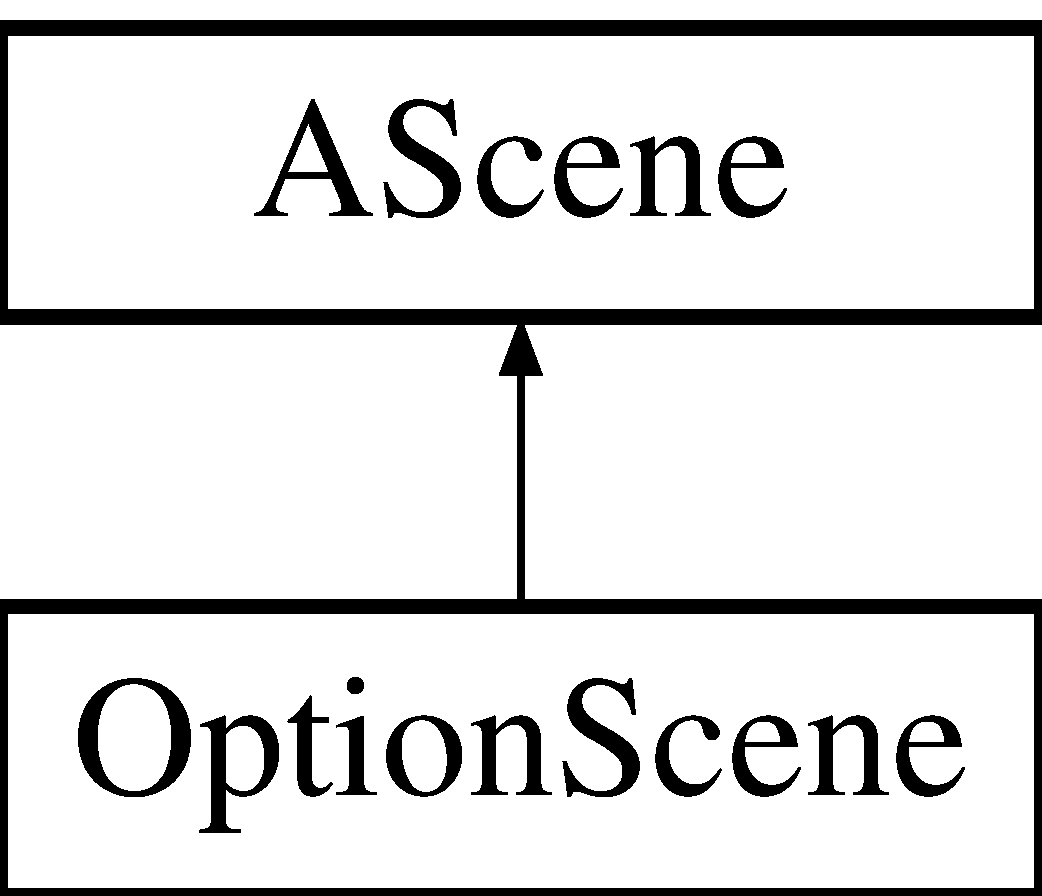
\includegraphics[height=2.000000cm]{classOptionScene}
\end{center}
\end{figure}
\subsection*{Public Member Functions}
\begin{DoxyCompactItemize}
\item 
\hyperlink{classOptionScene_ac0dfacf1988c5dcfe2520970735fab10}{Option\+Scene} ()
\begin{DoxyCompactList}\small\item\em Constructor. \end{DoxyCompactList}\item 
\hyperlink{classOptionScene_ab8de71400c4ed7f2a47cedfedb13f327}{$\sim$\+Option\+Scene} ()
\begin{DoxyCompactList}\small\item\em Destructor. \end{DoxyCompactList}\item 
\hyperlink{classirr_1_1IEventReceiver}{irr\+::\+I\+Event\+Receiver} $\ast$ \hyperlink{classOptionScene_a8848b9040ee7fd9c1d05a22181c5e053}{get\+Event\+Receiver} () const
\begin{DoxyCompactList}\small\item\em Event getter. \end{DoxyCompactList}\end{DoxyCompactItemize}


\subsection{Detailed Description}
\hyperlink{classButton}{Button} interface of option scene. 

\subsection{Constructor \& Destructor Documentation}
\mbox{\Hypertarget{classOptionScene_ac0dfacf1988c5dcfe2520970735fab10}\label{classOptionScene_ac0dfacf1988c5dcfe2520970735fab10}} 
\index{Option\+Scene@{Option\+Scene}!Option\+Scene@{Option\+Scene}}
\index{Option\+Scene@{Option\+Scene}!Option\+Scene@{Option\+Scene}}
\subsubsection{\texorpdfstring{Option\+Scene()}{OptionScene()}}
{\footnotesize\ttfamily Option\+Scene\+::\+Option\+Scene (\begin{DoxyParamCaption}{ }\end{DoxyParamCaption})}



Constructor. 

Build the class. \mbox{\Hypertarget{classOptionScene_ab8de71400c4ed7f2a47cedfedb13f327}\label{classOptionScene_ab8de71400c4ed7f2a47cedfedb13f327}} 
\index{Option\+Scene@{Option\+Scene}!````~Option\+Scene@{$\sim$\+Option\+Scene}}
\index{````~Option\+Scene@{$\sim$\+Option\+Scene}!Option\+Scene@{Option\+Scene}}
\subsubsection{\texorpdfstring{$\sim$\+Option\+Scene()}{~OptionScene()}}
{\footnotesize\ttfamily Option\+Scene\+::$\sim$\+Option\+Scene (\begin{DoxyParamCaption}{ }\end{DoxyParamCaption})}



Destructor. 

Destroy the class. 

\subsection{Member Function Documentation}
\mbox{\Hypertarget{classOptionScene_a8848b9040ee7fd9c1d05a22181c5e053}\label{classOptionScene_a8848b9040ee7fd9c1d05a22181c5e053}} 
\index{Option\+Scene@{Option\+Scene}!get\+Event\+Receiver@{get\+Event\+Receiver}}
\index{get\+Event\+Receiver@{get\+Event\+Receiver}!Option\+Scene@{Option\+Scene}}
\subsubsection{\texorpdfstring{get\+Event\+Receiver()}{getEventReceiver()}}
{\footnotesize\ttfamily \hyperlink{classirr_1_1IEventReceiver}{irr\+::\+I\+Event\+Receiver} $\ast$ Option\+Scene\+::get\+Event\+Receiver (\begin{DoxyParamCaption}{ }\end{DoxyParamCaption}) const\hspace{0.3cm}{\ttfamily [virtual]}}



Event getter. 

Return the event. 

Implements \hyperlink{classAScene_af521e5e6d30a5d2e5d30eb333e4d3abd}{A\+Scene}.



The documentation for this class was generated from the following files\+:\begin{DoxyCompactItemize}
\item 
inc/graphics/scenes/\hyperlink{OptionScene_8hh}{Option\+Scene.\+hh}\item 
src/graphics/scenes/Option\+Scene.\+cpp\end{DoxyCompactItemize}

\hypertarget{classOptionSoundReceiver}{}\section{Option\+Sound\+Receiver Class Reference}
\label{classOptionSoundReceiver}\index{Option\+Sound\+Receiver@{Option\+Sound\+Receiver}}


Manager of event of Sound scene setting.  




{\ttfamily \#include $<$Option\+Sound\+Receiver.\+hh$>$}



Inherits I\+Event\+Receiver.

\subsection*{Public Member Functions}
\begin{DoxyCompactItemize}
\item 
\hyperlink{classOptionSoundReceiver_aac72bf7db0c7610a37f9f14984f087ef}{Option\+Sound\+Receiver} (\hyperlink{classOptionSoundScene}{Option\+Sound\+Scene} $\ast$)
\begin{DoxyCompactList}\small\item\em Constructor. \end{DoxyCompactList}\item 
\hyperlink{classOptionSoundReceiver_aca3553e7a1777ed7e39111325b09954a}{$\sim$\+Option\+Sound\+Receiver} ()
\begin{DoxyCompactList}\small\item\em Destructor. \end{DoxyCompactList}\item 
bool \hyperlink{classOptionSoundReceiver_ae7c9643b12df38a45d4e3d629274019c}{On\+Event} (const irr\+::\+S\+Event \&event)
\begin{DoxyCompactList}\small\item\em Allow the user to handle envent into a scene. \end{DoxyCompactList}\end{DoxyCompactItemize}


\subsection{Detailed Description}
Manager of event of Sound scene setting. 

\subsection{Constructor \& Destructor Documentation}
\mbox{\Hypertarget{classOptionSoundReceiver_aac72bf7db0c7610a37f9f14984f087ef}\label{classOptionSoundReceiver_aac72bf7db0c7610a37f9f14984f087ef}} 
\index{Option\+Sound\+Receiver@{Option\+Sound\+Receiver}!Option\+Sound\+Receiver@{Option\+Sound\+Receiver}}
\index{Option\+Sound\+Receiver@{Option\+Sound\+Receiver}!Option\+Sound\+Receiver@{Option\+Sound\+Receiver}}
\subsubsection{\texorpdfstring{Option\+Sound\+Receiver()}{OptionSoundReceiver()}}
{\footnotesize\ttfamily Option\+Sound\+Receiver\+::\+Option\+Sound\+Receiver (\begin{DoxyParamCaption}\item[{\hyperlink{classOptionSoundScene}{Option\+Sound\+Scene} $\ast$}]{scene }\end{DoxyParamCaption})}



Constructor. 

Build the class. \mbox{\Hypertarget{classOptionSoundReceiver_aca3553e7a1777ed7e39111325b09954a}\label{classOptionSoundReceiver_aca3553e7a1777ed7e39111325b09954a}} 
\index{Option\+Sound\+Receiver@{Option\+Sound\+Receiver}!````~Option\+Sound\+Receiver@{$\sim$\+Option\+Sound\+Receiver}}
\index{````~Option\+Sound\+Receiver@{$\sim$\+Option\+Sound\+Receiver}!Option\+Sound\+Receiver@{Option\+Sound\+Receiver}}
\subsubsection{\texorpdfstring{$\sim$\+Option\+Sound\+Receiver()}{~OptionSoundReceiver()}}
{\footnotesize\ttfamily Option\+Sound\+Receiver\+::$\sim$\+Option\+Sound\+Receiver (\begin{DoxyParamCaption}{ }\end{DoxyParamCaption})}



Destructor. 

Destroy the class. 

\subsection{Member Function Documentation}
\mbox{\Hypertarget{classOptionSoundReceiver_ae7c9643b12df38a45d4e3d629274019c}\label{classOptionSoundReceiver_ae7c9643b12df38a45d4e3d629274019c}} 
\index{Option\+Sound\+Receiver@{Option\+Sound\+Receiver}!On\+Event@{On\+Event}}
\index{On\+Event@{On\+Event}!Option\+Sound\+Receiver@{Option\+Sound\+Receiver}}
\subsubsection{\texorpdfstring{On\+Event()}{OnEvent()}}
{\footnotesize\ttfamily bool Option\+Sound\+Receiver\+::\+On\+Event (\begin{DoxyParamCaption}\item[{const irr\+::\+S\+Event \&}]{event }\end{DoxyParamCaption})}



Allow the user to handle envent into a scene. 

Return true if he know the event, false if not. 

The documentation for this class was generated from the following files\+:\begin{DoxyCompactItemize}
\item 
inc/graphics/scenes/events/\hyperlink{OptionSoundReceiver_8hh}{Option\+Sound\+Receiver.\+hh}\item 
src/graphics/scenes/events/Option\+Sound\+Receiver.\+cpp\end{DoxyCompactItemize}

\hypertarget{classOptionSoundScene}{}\section{Option\+Sound\+Scene Class Reference}
\label{classOptionSoundScene}\index{Option\+Sound\+Scene@{Option\+Sound\+Scene}}


\hyperlink{classButton}{Button} interface of sound setting scene.  




{\ttfamily \#include $<$Option\+Sound\+Scene.\+hh$>$}

Inheritance diagram for Option\+Sound\+Scene\+:\begin{figure}[H]
\begin{center}
\leavevmode
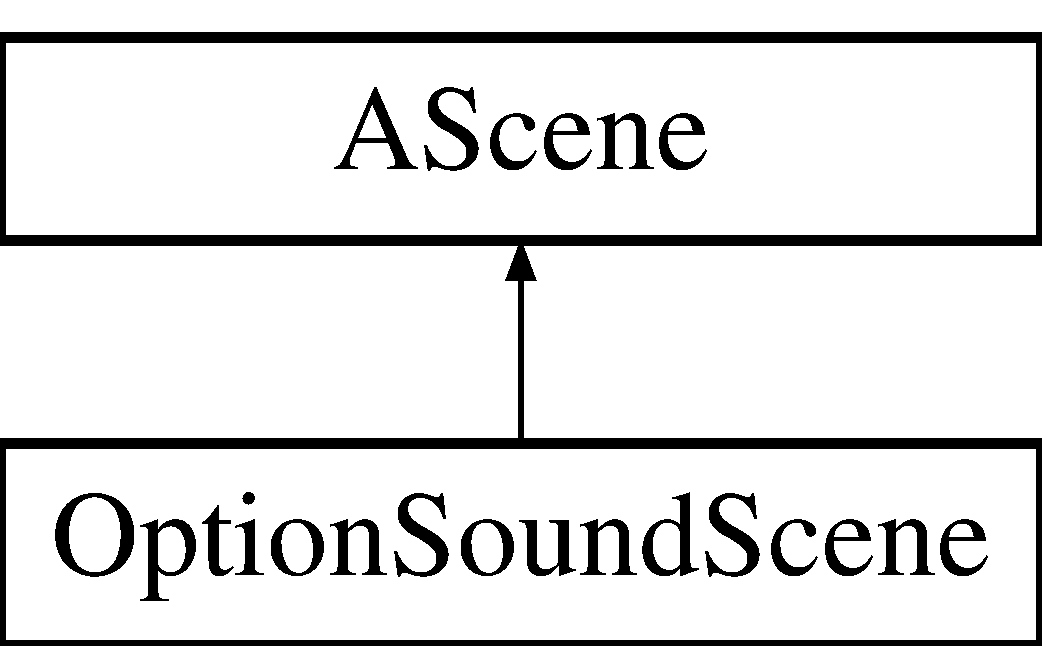
\includegraphics[height=2.000000cm]{classOptionSoundScene}
\end{center}
\end{figure}
\subsection*{Public Member Functions}
\begin{DoxyCompactItemize}
\item 
\hyperlink{classOptionSoundScene_abb8409b9b9225118e2779a1e0e7a4b45}{Option\+Sound\+Scene} ()
\begin{DoxyCompactList}\small\item\em Constructor. \end{DoxyCompactList}\item 
\hyperlink{classOptionSoundScene_afaf96649164e48bb5820cca80bc5c024}{$\sim$\+Option\+Sound\+Scene} ()
\begin{DoxyCompactList}\small\item\em Destructor. \end{DoxyCompactList}\item 
irr\+::\+I\+Event\+Receiver $\ast$ \hyperlink{classOptionSoundScene_ac71da65763f0db4b05fc32444308b677}{get\+Event\+Receiver} () const
\begin{DoxyCompactList}\small\item\em Allow the user to implemente the event callback class for each scene. \end{DoxyCompactList}\end{DoxyCompactItemize}


\subsection{Detailed Description}
\hyperlink{classButton}{Button} interface of sound setting scene. 

\subsection{Constructor \& Destructor Documentation}
\mbox{\Hypertarget{classOptionSoundScene_abb8409b9b9225118e2779a1e0e7a4b45}\label{classOptionSoundScene_abb8409b9b9225118e2779a1e0e7a4b45}} 
\index{Option\+Sound\+Scene@{Option\+Sound\+Scene}!Option\+Sound\+Scene@{Option\+Sound\+Scene}}
\index{Option\+Sound\+Scene@{Option\+Sound\+Scene}!Option\+Sound\+Scene@{Option\+Sound\+Scene}}
\subsubsection{\texorpdfstring{Option\+Sound\+Scene()}{OptionSoundScene()}}
{\footnotesize\ttfamily Option\+Sound\+Scene\+::\+Option\+Sound\+Scene (\begin{DoxyParamCaption}{ }\end{DoxyParamCaption})}



Constructor. 

Build the class. \mbox{\Hypertarget{classOptionSoundScene_afaf96649164e48bb5820cca80bc5c024}\label{classOptionSoundScene_afaf96649164e48bb5820cca80bc5c024}} 
\index{Option\+Sound\+Scene@{Option\+Sound\+Scene}!````~Option\+Sound\+Scene@{$\sim$\+Option\+Sound\+Scene}}
\index{````~Option\+Sound\+Scene@{$\sim$\+Option\+Sound\+Scene}!Option\+Sound\+Scene@{Option\+Sound\+Scene}}
\subsubsection{\texorpdfstring{$\sim$\+Option\+Sound\+Scene()}{~OptionSoundScene()}}
{\footnotesize\ttfamily Option\+Sound\+Scene\+::$\sim$\+Option\+Sound\+Scene (\begin{DoxyParamCaption}{ }\end{DoxyParamCaption})}



Destructor. 

Destroy the class. 

\subsection{Member Function Documentation}
\mbox{\Hypertarget{classOptionSoundScene_ac71da65763f0db4b05fc32444308b677}\label{classOptionSoundScene_ac71da65763f0db4b05fc32444308b677}} 
\index{Option\+Sound\+Scene@{Option\+Sound\+Scene}!get\+Event\+Receiver@{get\+Event\+Receiver}}
\index{get\+Event\+Receiver@{get\+Event\+Receiver}!Option\+Sound\+Scene@{Option\+Sound\+Scene}}
\subsubsection{\texorpdfstring{get\+Event\+Receiver()}{getEventReceiver()}}
{\footnotesize\ttfamily irr\+::\+I\+Event\+Receiver $\ast$ Option\+Sound\+Scene\+::get\+Event\+Receiver (\begin{DoxyParamCaption}{ }\end{DoxyParamCaption}) const\hspace{0.3cm}{\ttfamily [virtual]}}



Allow the user to implemente the event callback class for each scene. 

Return the event\textquotesingle{}s receiver. 

Implements \hyperlink{classAScene_af521e5e6d30a5d2e5d30eb333e4d3abd}{A\+Scene}.



The documentation for this class was generated from the following files\+:\begin{DoxyCompactItemize}
\item 
inc/graphics/scenes/\hyperlink{OptionSoundScene_8hh}{Option\+Sound\+Scene.\+hh}\item 
src/graphics/scenes/Option\+Sound\+Scene.\+cpp\end{DoxyCompactItemize}

\hypertarget{classOptionVideoReceiver}{}\section{Option\+Video\+Receiver Class Reference}
\label{classOptionVideoReceiver}\index{Option\+Video\+Receiver@{Option\+Video\+Receiver}}


Manager of event of video setting scene.  




{\ttfamily \#include $<$Option\+Video\+Receiver.\+hh$>$}



Inherits I\+Event\+Receiver.

\subsection*{Public Member Functions}
\begin{DoxyCompactItemize}
\item 
\hyperlink{classOptionVideoReceiver_ac513ff2e3b42ab38dc47b07ece611a61}{Option\+Video\+Receiver} ()
\begin{DoxyCompactList}\small\item\em Constructor. \end{DoxyCompactList}\item 
\hyperlink{classOptionVideoReceiver_ab014b77305c68f220fa5a0c8e9e57cb9}{$\sim$\+Option\+Video\+Receiver} ()
\begin{DoxyCompactList}\small\item\em Destructor. \end{DoxyCompactList}\item 
bool \hyperlink{classOptionVideoReceiver_a203025900c489eb2df12a6b3471c3caa}{On\+Event} (const irr\+::\+S\+Event \&event)
\begin{DoxyCompactList}\small\item\em Event manager. \end{DoxyCompactList}\end{DoxyCompactItemize}


\subsection{Detailed Description}
Manager of event of video setting scene. 

\subsection{Constructor \& Destructor Documentation}
\mbox{\Hypertarget{classOptionVideoReceiver_ac513ff2e3b42ab38dc47b07ece611a61}\label{classOptionVideoReceiver_ac513ff2e3b42ab38dc47b07ece611a61}} 
\index{Option\+Video\+Receiver@{Option\+Video\+Receiver}!Option\+Video\+Receiver@{Option\+Video\+Receiver}}
\index{Option\+Video\+Receiver@{Option\+Video\+Receiver}!Option\+Video\+Receiver@{Option\+Video\+Receiver}}
\subsubsection{\texorpdfstring{Option\+Video\+Receiver()}{OptionVideoReceiver()}}
{\footnotesize\ttfamily Option\+Video\+Receiver\+::\+Option\+Video\+Receiver (\begin{DoxyParamCaption}{ }\end{DoxyParamCaption})}



Constructor. 

Build the class. \mbox{\Hypertarget{classOptionVideoReceiver_ab014b77305c68f220fa5a0c8e9e57cb9}\label{classOptionVideoReceiver_ab014b77305c68f220fa5a0c8e9e57cb9}} 
\index{Option\+Video\+Receiver@{Option\+Video\+Receiver}!````~Option\+Video\+Receiver@{$\sim$\+Option\+Video\+Receiver}}
\index{````~Option\+Video\+Receiver@{$\sim$\+Option\+Video\+Receiver}!Option\+Video\+Receiver@{Option\+Video\+Receiver}}
\subsubsection{\texorpdfstring{$\sim$\+Option\+Video\+Receiver()}{~OptionVideoReceiver()}}
{\footnotesize\ttfamily Option\+Video\+Receiver\+::$\sim$\+Option\+Video\+Receiver (\begin{DoxyParamCaption}{ }\end{DoxyParamCaption})}



Destructor. 

Destroy the class. 

\subsection{Member Function Documentation}
\mbox{\Hypertarget{classOptionVideoReceiver_a203025900c489eb2df12a6b3471c3caa}\label{classOptionVideoReceiver_a203025900c489eb2df12a6b3471c3caa}} 
\index{Option\+Video\+Receiver@{Option\+Video\+Receiver}!On\+Event@{On\+Event}}
\index{On\+Event@{On\+Event}!Option\+Video\+Receiver@{Option\+Video\+Receiver}}
\subsubsection{\texorpdfstring{On\+Event()}{OnEvent()}}
{\footnotesize\ttfamily bool Option\+Video\+Receiver\+::\+On\+Event (\begin{DoxyParamCaption}\item[{const irr\+::\+S\+Event \&}]{event }\end{DoxyParamCaption})}



Event manager. 

Return true if he know the event, false if not. 

The documentation for this class was generated from the following files\+:\begin{DoxyCompactItemize}
\item 
inc/graphics/scenes/events/\hyperlink{OptionVideoReceiver_8hh}{Option\+Video\+Receiver.\+hh}\item 
src/graphics/scenes/events/Option\+Video\+Receiver.\+cpp\end{DoxyCompactItemize}

\hypertarget{classOptionVideoScene}{}\section{Option\+Video\+Scene Class Reference}
\label{classOptionVideoScene}\index{Option\+Video\+Scene@{Option\+Video\+Scene}}


\hyperlink{classButton}{Button} interface of video setting scene.  




{\ttfamily \#include $<$Option\+Video\+Scene.\+hh$>$}

Inheritance diagram for Option\+Video\+Scene\+:\begin{figure}[H]
\begin{center}
\leavevmode
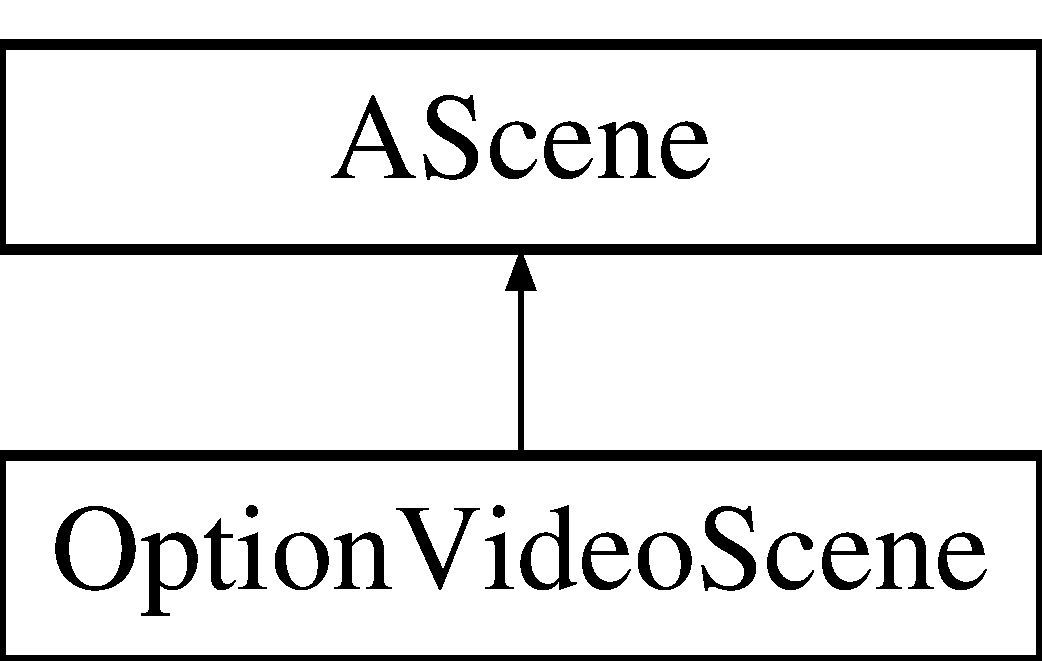
\includegraphics[height=2.000000cm]{classOptionVideoScene}
\end{center}
\end{figure}
\subsection*{Public Member Functions}
\begin{DoxyCompactItemize}
\item 
\hyperlink{classOptionVideoScene_a4adc5d02ab700ef59733b19183769dea}{Option\+Video\+Scene} ()
\begin{DoxyCompactList}\small\item\em Constructor. \end{DoxyCompactList}\item 
\hyperlink{classOptionVideoScene_aaafd7499ea05590a0d61109ae7bcbf08}{$\sim$\+Option\+Video\+Scene} ()
\begin{DoxyCompactList}\small\item\em Destructor. \end{DoxyCompactList}\item 
irr\+::\+I\+Event\+Receiver $\ast$ \hyperlink{classOptionVideoScene_a84625e871c5176d7abc77a7f12c1472a}{get\+Event\+Receiver} () const
\begin{DoxyCompactList}\small\item\em Allow the user to implemente the event callback class for each scene. \end{DoxyCompactList}\end{DoxyCompactItemize}


\subsection{Detailed Description}
\hyperlink{classButton}{Button} interface of video setting scene. 

\subsection{Constructor \& Destructor Documentation}
\mbox{\Hypertarget{classOptionVideoScene_a4adc5d02ab700ef59733b19183769dea}\label{classOptionVideoScene_a4adc5d02ab700ef59733b19183769dea}} 
\index{Option\+Video\+Scene@{Option\+Video\+Scene}!Option\+Video\+Scene@{Option\+Video\+Scene}}
\index{Option\+Video\+Scene@{Option\+Video\+Scene}!Option\+Video\+Scene@{Option\+Video\+Scene}}
\subsubsection{\texorpdfstring{Option\+Video\+Scene()}{OptionVideoScene()}}
{\footnotesize\ttfamily Option\+Video\+Scene\+::\+Option\+Video\+Scene (\begin{DoxyParamCaption}{ }\end{DoxyParamCaption})}



Constructor. 

Build the class. \mbox{\Hypertarget{classOptionVideoScene_aaafd7499ea05590a0d61109ae7bcbf08}\label{classOptionVideoScene_aaafd7499ea05590a0d61109ae7bcbf08}} 
\index{Option\+Video\+Scene@{Option\+Video\+Scene}!````~Option\+Video\+Scene@{$\sim$\+Option\+Video\+Scene}}
\index{````~Option\+Video\+Scene@{$\sim$\+Option\+Video\+Scene}!Option\+Video\+Scene@{Option\+Video\+Scene}}
\subsubsection{\texorpdfstring{$\sim$\+Option\+Video\+Scene()}{~OptionVideoScene()}}
{\footnotesize\ttfamily Option\+Video\+Scene\+::$\sim$\+Option\+Video\+Scene (\begin{DoxyParamCaption}{ }\end{DoxyParamCaption})}



Destructor. 

Destroy the class. 

\subsection{Member Function Documentation}
\mbox{\Hypertarget{classOptionVideoScene_a84625e871c5176d7abc77a7f12c1472a}\label{classOptionVideoScene_a84625e871c5176d7abc77a7f12c1472a}} 
\index{Option\+Video\+Scene@{Option\+Video\+Scene}!get\+Event\+Receiver@{get\+Event\+Receiver}}
\index{get\+Event\+Receiver@{get\+Event\+Receiver}!Option\+Video\+Scene@{Option\+Video\+Scene}}
\subsubsection{\texorpdfstring{get\+Event\+Receiver()}{getEventReceiver()}}
{\footnotesize\ttfamily irr\+::\+I\+Event\+Receiver $\ast$ Option\+Video\+Scene\+::get\+Event\+Receiver (\begin{DoxyParamCaption}{ }\end{DoxyParamCaption}) const\hspace{0.3cm}{\ttfamily [virtual]}}



Allow the user to implemente the event callback class for each scene. 

Return the event. 

Implements \hyperlink{classAScene_af521e5e6d30a5d2e5d30eb333e4d3abd}{A\+Scene}.



The documentation for this class was generated from the following files\+:\begin{DoxyCompactItemize}
\item 
inc/graphics/scenes/\hyperlink{OptionVideoScene_8hh}{Option\+Video\+Scene.\+hh}\item 
src/graphics/scenes/Option\+Video\+Scene.\+cpp\end{DoxyCompactItemize}

\hypertarget{classPotion}{}\section{Potion Class Reference}
\label{classPotion}\index{Potion@{Potion}}


create a \hyperlink{classAPickable}{A\+Pickable} \hyperlink{classAObject}{A\+Object} key  




{\ttfamily \#include $<$Potion.\+hh$>$}

Inheritance diagram for Potion\+:\begin{figure}[H]
\begin{center}
\leavevmode
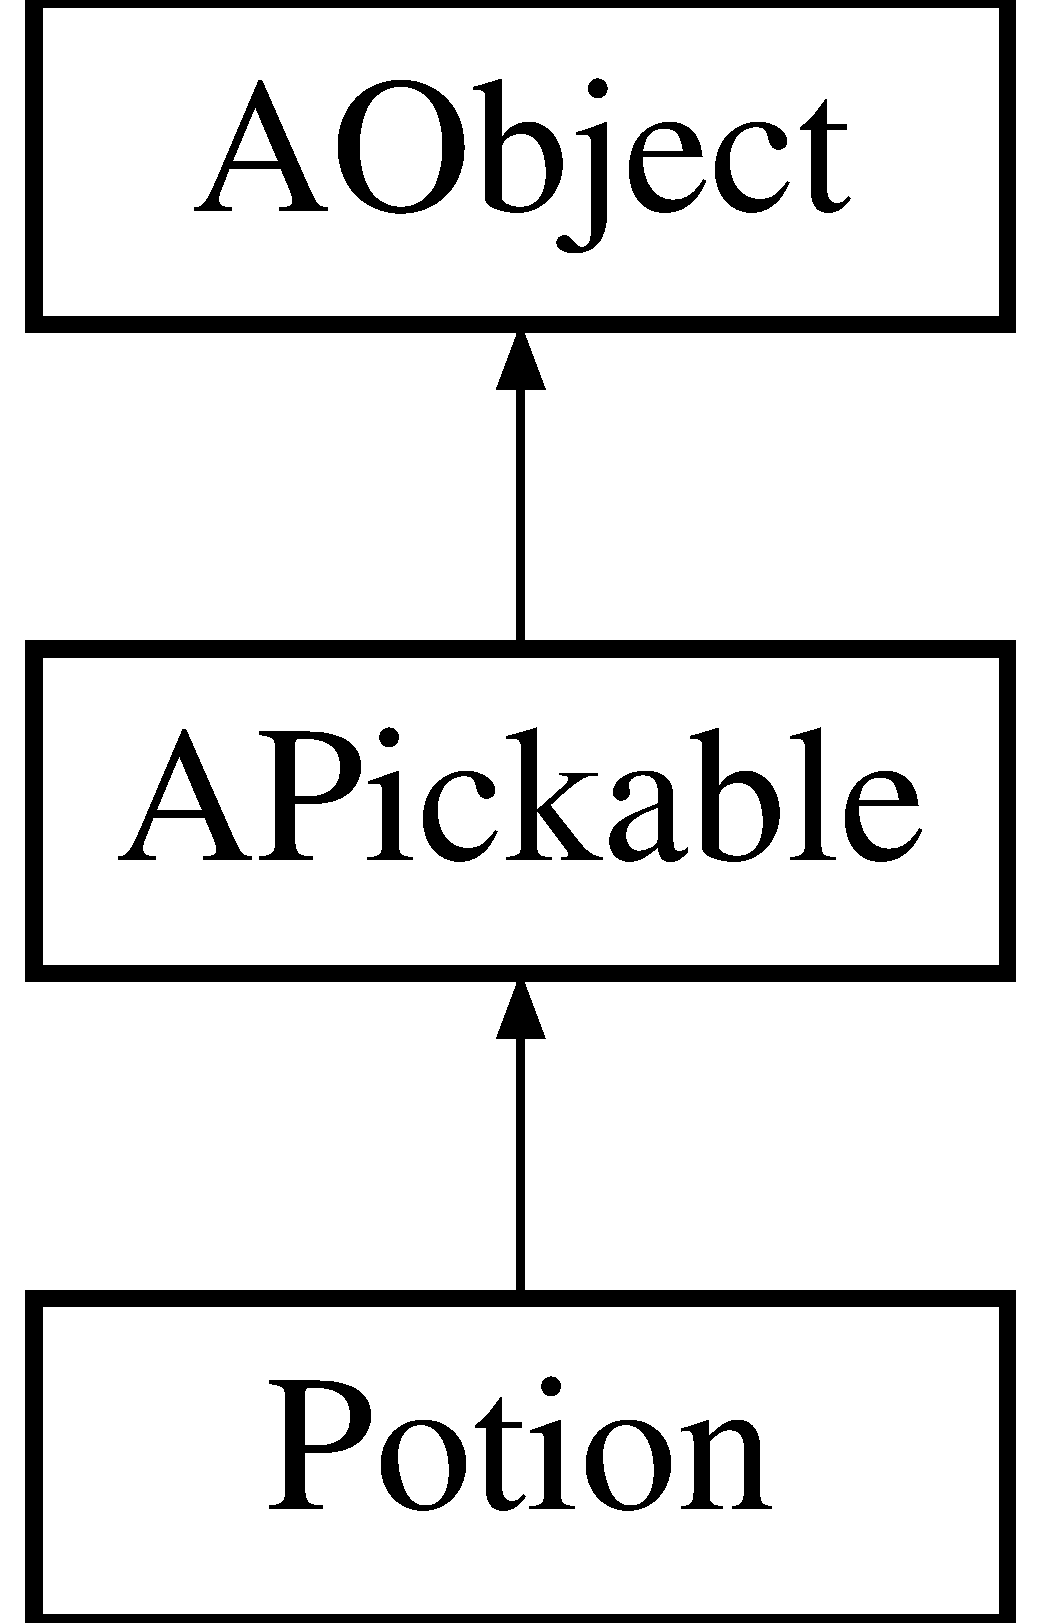
\includegraphics[height=3.000000cm]{classPotion}
\end{center}
\end{figure}
\subsection*{Public Member Functions}
\begin{DoxyCompactItemize}
\item 
\hyperlink{classPotion_a2fae017a2dbe6fd82269d19a51908959}{Potion} (\hyperlink{namespaceirr_ac66849b7a6ed16e30ebede579f9b47c6}{irr\+::s32} regen\+Point, indie\+::potion\+Type type=indie\+::potion\+Type\+::\+L\+I\+FE, \hyperlink{namespaceirr_a0416a53257075833e7002efd0a18e804}{irr\+::u32} id=0)
\begin{DoxyCompactList}\small\item\em Constructor. \end{DoxyCompactList}\item 
\hyperlink{classPotion_a8730c8052ec698171885bb5dacda9cca}{$\sim$\+Potion} ()
\begin{DoxyCompactList}\small\item\em Destructor. \end{DoxyCompactList}\end{DoxyCompactItemize}


\subsection{Detailed Description}
create a \hyperlink{classAPickable}{A\+Pickable} \hyperlink{classAObject}{A\+Object} key 

\subsection{Constructor \& Destructor Documentation}
\mbox{\Hypertarget{classPotion_a2fae017a2dbe6fd82269d19a51908959}\label{classPotion_a2fae017a2dbe6fd82269d19a51908959}} 
\index{Potion@{Potion}!Potion@{Potion}}
\index{Potion@{Potion}!Potion@{Potion}}
\subsubsection{\texorpdfstring{Potion()}{Potion()}}
{\footnotesize\ttfamily Potion\+::\+Potion (\begin{DoxyParamCaption}\item[{\hyperlink{namespaceirr_ac66849b7a6ed16e30ebede579f9b47c6}{irr\+::s32}}]{regen\+Point,  }\item[{indie\+::potion\+Type}]{type = {\ttfamily indie\+:\+:potionType\+:\+:LIFE},  }\item[{\hyperlink{namespaceirr_a0416a53257075833e7002efd0a18e804}{irr\+::u32}}]{id = {\ttfamily 0} }\end{DoxyParamCaption})}



Constructor. 

Build the class, first param is number of regen\+Point, second the type of potion (L\+I\+FE, M\+A\+NA, P\+O\+W\+ER) \mbox{\Hypertarget{classPotion_a8730c8052ec698171885bb5dacda9cca}\label{classPotion_a8730c8052ec698171885bb5dacda9cca}} 
\index{Potion@{Potion}!````~Potion@{$\sim$\+Potion}}
\index{````~Potion@{$\sim$\+Potion}!Potion@{Potion}}
\subsubsection{\texorpdfstring{$\sim$\+Potion()}{~Potion()}}
{\footnotesize\ttfamily Potion\+::$\sim$\+Potion (\begin{DoxyParamCaption}{ }\end{DoxyParamCaption})}



Destructor. 

Destroy a class 

The documentation for this class was generated from the following files\+:\begin{DoxyCompactItemize}
\item 
inc/game/object/Potion.\+hh\item 
src/game/object/Potion.\+cpp\end{DoxyCompactItemize}

\hypertarget{classSaveManager}{}\section{Save\+Manager Class Reference}
\label{classSaveManager}\index{Save\+Manager@{Save\+Manager}}


The \hyperlink{classSaveManager}{Save\+Manager} class.  




{\ttfamily \#include $<$Save\+Manager.\+hh$>$}

\subsection*{Public Member Functions}
\begin{DoxyCompactItemize}
\item 
\mbox{\Hypertarget{classSaveManager_ab8bb791be648b9b91db44aa11f6e8e14}\label{classSaveManager_ab8bb791be648b9b91db44aa11f6e8e14}} 
\hyperlink{classSaveManager_ab8bb791be648b9b91db44aa11f6e8e14}{Save\+Manager} ()
\begin{DoxyCompactList}\small\item\em The constructor. \end{DoxyCompactList}\item 
void \hyperlink{classSaveManager_a96c17debbf9765e8c71e74010621585f}{load\+Games} (std\+::string folder)
\begin{DoxyCompactList}\small\item\em Allow you to load a game previously save. \end{DoxyCompactList}\item 
\mbox{\Hypertarget{classSaveManager_a43beb7dd453f37de97c3a8de3b1142ab}\label{classSaveManager_a43beb7dd453f37de97c3a8de3b1142ab}} 
void \hyperlink{classSaveManager_a43beb7dd453f37de97c3a8de3b1142ab}{save\+Games} ()
\begin{DoxyCompactList}\small\item\em Allow you to save all the games previously load. \end{DoxyCompactList}\item 
\mbox{\Hypertarget{classSaveManager_a7b950ce71223640fe56e8d404fe3cd2f}\label{classSaveManager_a7b950ce71223640fe56e8d404fe3cd2f}} 
const std\+::shared\+\_\+ptr$<$ \hyperlink{classGame}{Game} $>$ \hyperlink{classSaveManager_a7b950ce71223640fe56e8d404fe3cd2f}{get\+Game} ()
\begin{DoxyCompactList}\small\item\em Return a pointeur to the current game. \end{DoxyCompactList}\item 
const std\+::shared\+\_\+ptr$<$ std\+::vector$<$ std\+::string $>$ $>$ \hyperlink{classSaveManager_a335611df31b6a1eccb5c7df73bc2e778}{get\+Saves\+Names} ()
\begin{DoxyCompactList}\small\item\em Allow you to get the names of all the saves. \end{DoxyCompactList}\end{DoxyCompactItemize}


\subsection{Detailed Description}
The \hyperlink{classSaveManager}{Save\+Manager} class. 

\subsection{Member Function Documentation}
\mbox{\Hypertarget{classSaveManager_a335611df31b6a1eccb5c7df73bc2e778}\label{classSaveManager_a335611df31b6a1eccb5c7df73bc2e778}} 
\index{Save\+Manager@{Save\+Manager}!get\+Saves\+Names@{get\+Saves\+Names}}
\index{get\+Saves\+Names@{get\+Saves\+Names}!Save\+Manager@{Save\+Manager}}
\subsubsection{\texorpdfstring{get\+Saves\+Names()}{getSavesNames()}}
{\footnotesize\ttfamily const std\+::shared\+\_\+ptr$<$ std\+::vector$<$ std\+::string $>$ $>$ Save\+Manager\+::get\+Saves\+Names (\begin{DoxyParamCaption}{ }\end{DoxyParamCaption})}



Allow you to get the names of all the saves. 

\begin{DoxyReturn}{Returns}
A vector with all the names 
\end{DoxyReturn}
\mbox{\Hypertarget{classSaveManager_a96c17debbf9765e8c71e74010621585f}\label{classSaveManager_a96c17debbf9765e8c71e74010621585f}} 
\index{Save\+Manager@{Save\+Manager}!load\+Games@{load\+Games}}
\index{load\+Games@{load\+Games}!Save\+Manager@{Save\+Manager}}
\subsubsection{\texorpdfstring{load\+Games()}{loadGames()}}
{\footnotesize\ttfamily void Save\+Manager\+::load\+Games (\begin{DoxyParamCaption}\item[{std\+::string}]{folder }\end{DoxyParamCaption})}



Allow you to load a game previously save. 


\begin{DoxyParams}{Parameters}
{\em folder} & Path to a folders were all the xml are \\
\hline
\end{DoxyParams}


The documentation for this class was generated from the following files\+:\begin{DoxyCompactItemize}
\item 
inc/managers/\hyperlink{SaveManager_8hh}{Save\+Manager.\+hh}\item 
src/managers/Save\+Manager.\+cpp\end{DoxyCompactItemize}

\hypertarget{classScoreManager}{}\section{Score\+Manager Class Reference}
\label{classScoreManager}\index{Score\+Manager@{Score\+Manager}}


The \hyperlink{classScoreManager}{Score\+Manager} class.  




{\ttfamily \#include $<$Score\+Manager.\+hh$>$}

\subsection*{Public Member Functions}
\begin{DoxyCompactItemize}
\item 
\hyperlink{classScoreManager_a4f3866ff832127664543349da5c4fbf4}{Score\+Manager} ()
\begin{DoxyCompactList}\small\item\em The constructor. \end{DoxyCompactList}\item 
void \hyperlink{classScoreManager_a3644cf37cdce0983dc8ed3005222e55a}{load\+Scores} (std\+::string)
\begin{DoxyCompactList}\small\item\em Allow you to load a score sheet (from a previous session) \end{DoxyCompactList}\item 
\mbox{\Hypertarget{classScoreManager_aa3f390fe5076324b2d457de0c43af59f}\label{classScoreManager_aa3f390fe5076324b2d457de0c43af59f}} 
void \hyperlink{classScoreManager_aa3f390fe5076324b2d457de0c43af59f}{save\+Scores} () const
\begin{DoxyCompactList}\small\item\em Allow you to save the score contained in the object. \end{DoxyCompactList}\item 
void \hyperlink{classScoreManager_a93810ab5b58af22f8af96db0787363b8}{create\+File} (std\+::string)
\begin{DoxyCompactList}\small\item\em Create an empty score file. \end{DoxyCompactList}\item 
void \hyperlink{classScoreManager_a2597a2f7d0786295a6ee3445502a6d6f}{add\+Score} (std\+::string, std\+::size\+\_\+t)
\begin{DoxyCompactList}\small\item\em Add a score. \end{DoxyCompactList}\item 
\mbox{\Hypertarget{classScoreManager_ad0c38dd0a27a82230d09f29ce3d12349}\label{classScoreManager_ad0c38dd0a27a82230d09f29ce3d12349}} 
const std\+::vector$<$ config\+::\+Score $>$ \& \hyperlink{classScoreManager_ad0c38dd0a27a82230d09f29ce3d12349}{get\+Top\+Scores} ()
\begin{DoxyCompactList}\small\item\em Get the 10 best scores. \end{DoxyCompactList}\item 
std\+::size\+\_\+t \hyperlink{classScoreManager_a9d529f071418d69a2b1745673d9d83b2}{get\+Player\+Score} (std\+::string) const
\begin{DoxyCompactList}\small\item\em Get score for a specifique player. \end{DoxyCompactList}\item 
void \hyperlink{classScoreManager_a16c1e33b2972b9609b6d568dc8b7a3b0}{change\+Score} (std\+::string, std\+::size\+\_\+t)
\begin{DoxyCompactList}\small\item\em Change score for a specifique player. \end{DoxyCompactList}\end{DoxyCompactItemize}


\subsection{Detailed Description}
The \hyperlink{classScoreManager}{Score\+Manager} class. 

\subsection{Constructor \& Destructor Documentation}
\mbox{\Hypertarget{classScoreManager_a4f3866ff832127664543349da5c4fbf4}\label{classScoreManager_a4f3866ff832127664543349da5c4fbf4}} 
\index{Score\+Manager@{Score\+Manager}!Score\+Manager@{Score\+Manager}}
\index{Score\+Manager@{Score\+Manager}!Score\+Manager@{Score\+Manager}}
\subsubsection{\texorpdfstring{Score\+Manager()}{ScoreManager()}}
{\footnotesize\ttfamily Score\+Manager\+::\+Score\+Manager (\begin{DoxyParamCaption}{ }\end{DoxyParamCaption})}



The constructor. 


\begin{DoxyParams}{Parameters}
{\em Nothing} & \\
\hline
\end{DoxyParams}


\subsection{Member Function Documentation}
\mbox{\Hypertarget{classScoreManager_a2597a2f7d0786295a6ee3445502a6d6f}\label{classScoreManager_a2597a2f7d0786295a6ee3445502a6d6f}} 
\index{Score\+Manager@{Score\+Manager}!add\+Score@{add\+Score}}
\index{add\+Score@{add\+Score}!Score\+Manager@{Score\+Manager}}
\subsubsection{\texorpdfstring{add\+Score()}{addScore()}}
{\footnotesize\ttfamily void Score\+Manager\+::add\+Score (\begin{DoxyParamCaption}\item[{std\+::string}]{player\+Name,  }\item[{std\+::size\+\_\+t}]{player\+Score }\end{DoxyParamCaption})}



Add a score. 


\begin{DoxyParams}{Parameters}
{\em 1.} & Player name 2. Is score \\
\hline
\end{DoxyParams}
\mbox{\Hypertarget{classScoreManager_a16c1e33b2972b9609b6d568dc8b7a3b0}\label{classScoreManager_a16c1e33b2972b9609b6d568dc8b7a3b0}} 
\index{Score\+Manager@{Score\+Manager}!change\+Score@{change\+Score}}
\index{change\+Score@{change\+Score}!Score\+Manager@{Score\+Manager}}
\subsubsection{\texorpdfstring{change\+Score()}{changeScore()}}
{\footnotesize\ttfamily void Score\+Manager\+::change\+Score (\begin{DoxyParamCaption}\item[{std\+::string}]{,  }\item[{std\+::size\+\_\+t}]{ }\end{DoxyParamCaption})}



Change score for a specifique player. 


\begin{DoxyParams}{Parameters}
{\em 1.} & Player name 2. New score \\
\hline
\end{DoxyParams}
\mbox{\Hypertarget{classScoreManager_a93810ab5b58af22f8af96db0787363b8}\label{classScoreManager_a93810ab5b58af22f8af96db0787363b8}} 
\index{Score\+Manager@{Score\+Manager}!create\+File@{create\+File}}
\index{create\+File@{create\+File}!Score\+Manager@{Score\+Manager}}
\subsubsection{\texorpdfstring{create\+File()}{createFile()}}
{\footnotesize\ttfamily void Score\+Manager\+::create\+File (\begin{DoxyParamCaption}\item[{std\+::string}]{file\+Name }\end{DoxyParamCaption})}



Create an empty score file. 


\begin{DoxyParams}{Parameters}
{\em Path} & to the score file \\
\hline
\end{DoxyParams}
\mbox{\Hypertarget{classScoreManager_a9d529f071418d69a2b1745673d9d83b2}\label{classScoreManager_a9d529f071418d69a2b1745673d9d83b2}} 
\index{Score\+Manager@{Score\+Manager}!get\+Player\+Score@{get\+Player\+Score}}
\index{get\+Player\+Score@{get\+Player\+Score}!Score\+Manager@{Score\+Manager}}
\subsubsection{\texorpdfstring{get\+Player\+Score()}{getPlayerScore()}}
{\footnotesize\ttfamily std\+::size\+\_\+t Score\+Manager\+::get\+Player\+Score (\begin{DoxyParamCaption}\item[{std\+::string}]{name }\end{DoxyParamCaption}) const}



Get score for a specifique player. 


\begin{DoxyParams}{Parameters}
{\em Player} & name \\
\hline
\end{DoxyParams}
\mbox{\Hypertarget{classScoreManager_a3644cf37cdce0983dc8ed3005222e55a}\label{classScoreManager_a3644cf37cdce0983dc8ed3005222e55a}} 
\index{Score\+Manager@{Score\+Manager}!load\+Scores@{load\+Scores}}
\index{load\+Scores@{load\+Scores}!Score\+Manager@{Score\+Manager}}
\subsubsection{\texorpdfstring{load\+Scores()}{loadScores()}}
{\footnotesize\ttfamily void Score\+Manager\+::load\+Scores (\begin{DoxyParamCaption}\item[{std\+::string}]{file\+Name }\end{DoxyParamCaption})}



Allow you to load a score sheet (from a previous session) 


\begin{DoxyParams}{Parameters}
{\em The} & path to the score file \\
\hline
\end{DoxyParams}


The documentation for this class was generated from the following files\+:\begin{DoxyCompactItemize}
\item 
inc/managers/\hyperlink{ScoreManager_8hh}{Score\+Manager.\+hh}\item 
src/managers/Score\+Manager.\+cpp\end{DoxyCompactItemize}

\hypertarget{classScoreScene}{}\section{Score\+Scene Class Reference}
\label{classScoreScene}\index{Score\+Scene@{Score\+Scene}}


\hyperlink{classButton}{Button} interface of \hyperlink{classScoreScene}{Score\+Scene}.  




{\ttfamily \#include $<$Score\+Scene.\+hh$>$}

Inheritance diagram for Score\+Scene\+:\begin{figure}[H]
\begin{center}
\leavevmode
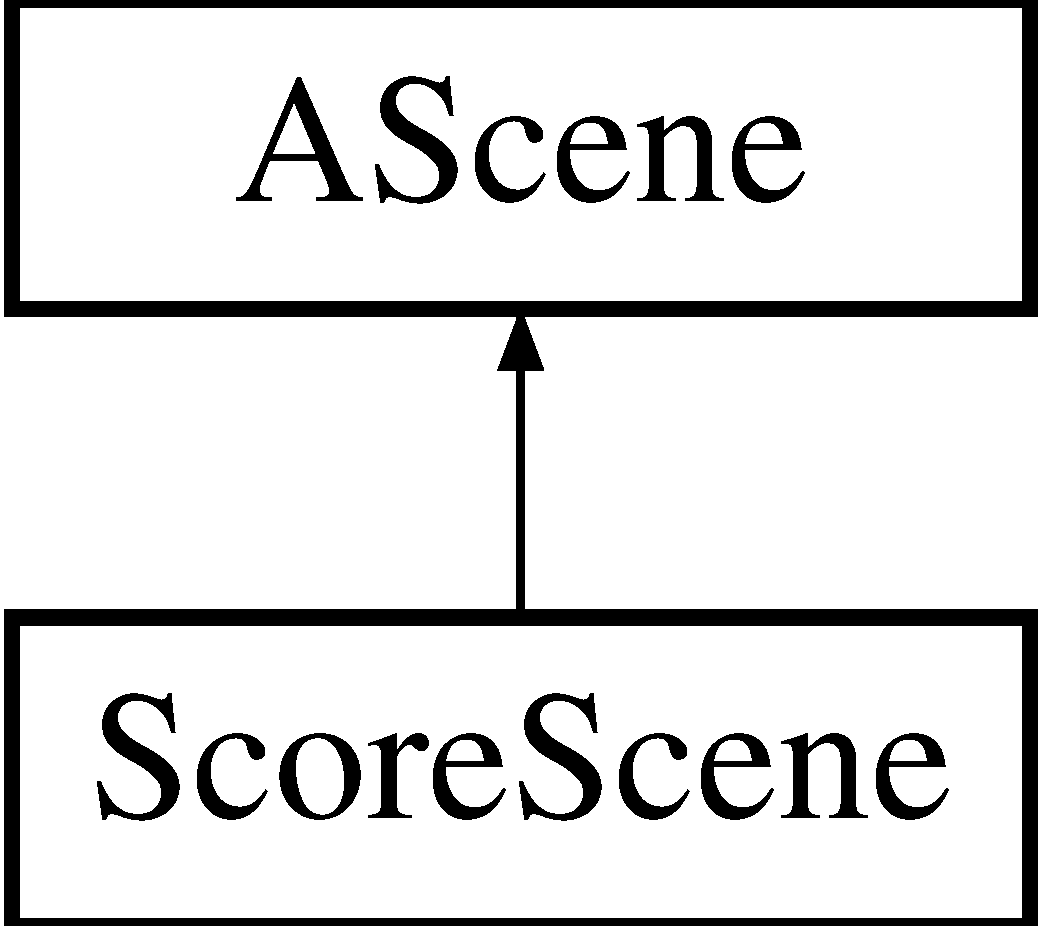
\includegraphics[height=2.000000cm]{classScoreScene}
\end{center}
\end{figure}
\subsection*{Public Member Functions}
\begin{DoxyCompactItemize}
\item 
\hyperlink{classScoreScene_a832799285cf03c37c18c83d0adde2baa}{Score\+Scene} ()
\begin{DoxyCompactList}\small\item\em Constructor. \end{DoxyCompactList}\item 
\hyperlink{classScoreScene_a1d3866f2c756fea86ec9adfb0a3eeb36}{$\sim$\+Score\+Scene} ()
\begin{DoxyCompactList}\small\item\em Destructor. \end{DoxyCompactList}\item 
irr\+::\+I\+Event\+Receiver $\ast$ \hyperlink{classScoreScene_ae398ba58a33b3605a0c71265202534e2}{get\+Event\+Receiver} () const
\begin{DoxyCompactList}\small\item\em Event getter. \end{DoxyCompactList}\item 
W\+String \hyperlink{classScoreScene_af82d6c841dc42c42d83202d2c7ddf8c9}{get\+Scores} () const
\begin{DoxyCompactList}\small\item\em Event getter. \end{DoxyCompactList}\end{DoxyCompactItemize}


\subsection{Detailed Description}
\hyperlink{classButton}{Button} interface of \hyperlink{classScoreScene}{Score\+Scene}. 

\subsection{Constructor \& Destructor Documentation}
\mbox{\Hypertarget{classScoreScene_a832799285cf03c37c18c83d0adde2baa}\label{classScoreScene_a832799285cf03c37c18c83d0adde2baa}} 
\index{Score\+Scene@{Score\+Scene}!Score\+Scene@{Score\+Scene}}
\index{Score\+Scene@{Score\+Scene}!Score\+Scene@{Score\+Scene}}
\subsubsection{\texorpdfstring{Score\+Scene()}{ScoreScene()}}
{\footnotesize\ttfamily Score\+Scene\+::\+Score\+Scene (\begin{DoxyParamCaption}{ }\end{DoxyParamCaption})}



Constructor. 

Build the class. \mbox{\Hypertarget{classScoreScene_a1d3866f2c756fea86ec9adfb0a3eeb36}\label{classScoreScene_a1d3866f2c756fea86ec9adfb0a3eeb36}} 
\index{Score\+Scene@{Score\+Scene}!````~Score\+Scene@{$\sim$\+Score\+Scene}}
\index{````~Score\+Scene@{$\sim$\+Score\+Scene}!Score\+Scene@{Score\+Scene}}
\subsubsection{\texorpdfstring{$\sim$\+Score\+Scene()}{~ScoreScene()}}
{\footnotesize\ttfamily Score\+Scene\+::$\sim$\+Score\+Scene (\begin{DoxyParamCaption}{ }\end{DoxyParamCaption})}



Destructor. 

Destroy the class. 

\subsection{Member Function Documentation}
\mbox{\Hypertarget{classScoreScene_ae398ba58a33b3605a0c71265202534e2}\label{classScoreScene_ae398ba58a33b3605a0c71265202534e2}} 
\index{Score\+Scene@{Score\+Scene}!get\+Event\+Receiver@{get\+Event\+Receiver}}
\index{get\+Event\+Receiver@{get\+Event\+Receiver}!Score\+Scene@{Score\+Scene}}
\subsubsection{\texorpdfstring{get\+Event\+Receiver()}{getEventReceiver()}}
{\footnotesize\ttfamily irr\+::\+I\+Event\+Receiver $\ast$ Score\+Scene\+::get\+Event\+Receiver (\begin{DoxyParamCaption}{ }\end{DoxyParamCaption}) const\hspace{0.3cm}{\ttfamily [virtual]}}



Event getter. 

Return the event. 

Implements \hyperlink{classAScene_af521e5e6d30a5d2e5d30eb333e4d3abd}{A\+Scene}.

\mbox{\Hypertarget{classScoreScene_af82d6c841dc42c42d83202d2c7ddf8c9}\label{classScoreScene_af82d6c841dc42c42d83202d2c7ddf8c9}} 
\index{Score\+Scene@{Score\+Scene}!get\+Scores@{get\+Scores}}
\index{get\+Scores@{get\+Scores}!Score\+Scene@{Score\+Scene}}
\subsubsection{\texorpdfstring{get\+Scores()}{getScores()}}
{\footnotesize\ttfamily W\+String Score\+Scene\+::get\+Scores (\begin{DoxyParamCaption}{ }\end{DoxyParamCaption}) const}



Event getter. 

Return the Score. 

The documentation for this class was generated from the following files\+:\begin{DoxyCompactItemize}
\item 
inc/graphics/scenes/\hyperlink{ScoreScene_8hh}{Score\+Scene.\+hh}\item 
src/graphics/scenes/Score\+Scene.\+cpp\end{DoxyCompactItemize}

\hypertarget{classText}{}\section{Text Class Reference}
\label{classText}\index{Text@{Text}}


Inherited from a \hyperlink{classIWidget}{I\+Widget}.  




{\ttfamily \#include $<$Text.\+hh$>$}

Inheritance diagram for Text\+:\begin{figure}[H]
\begin{center}
\leavevmode
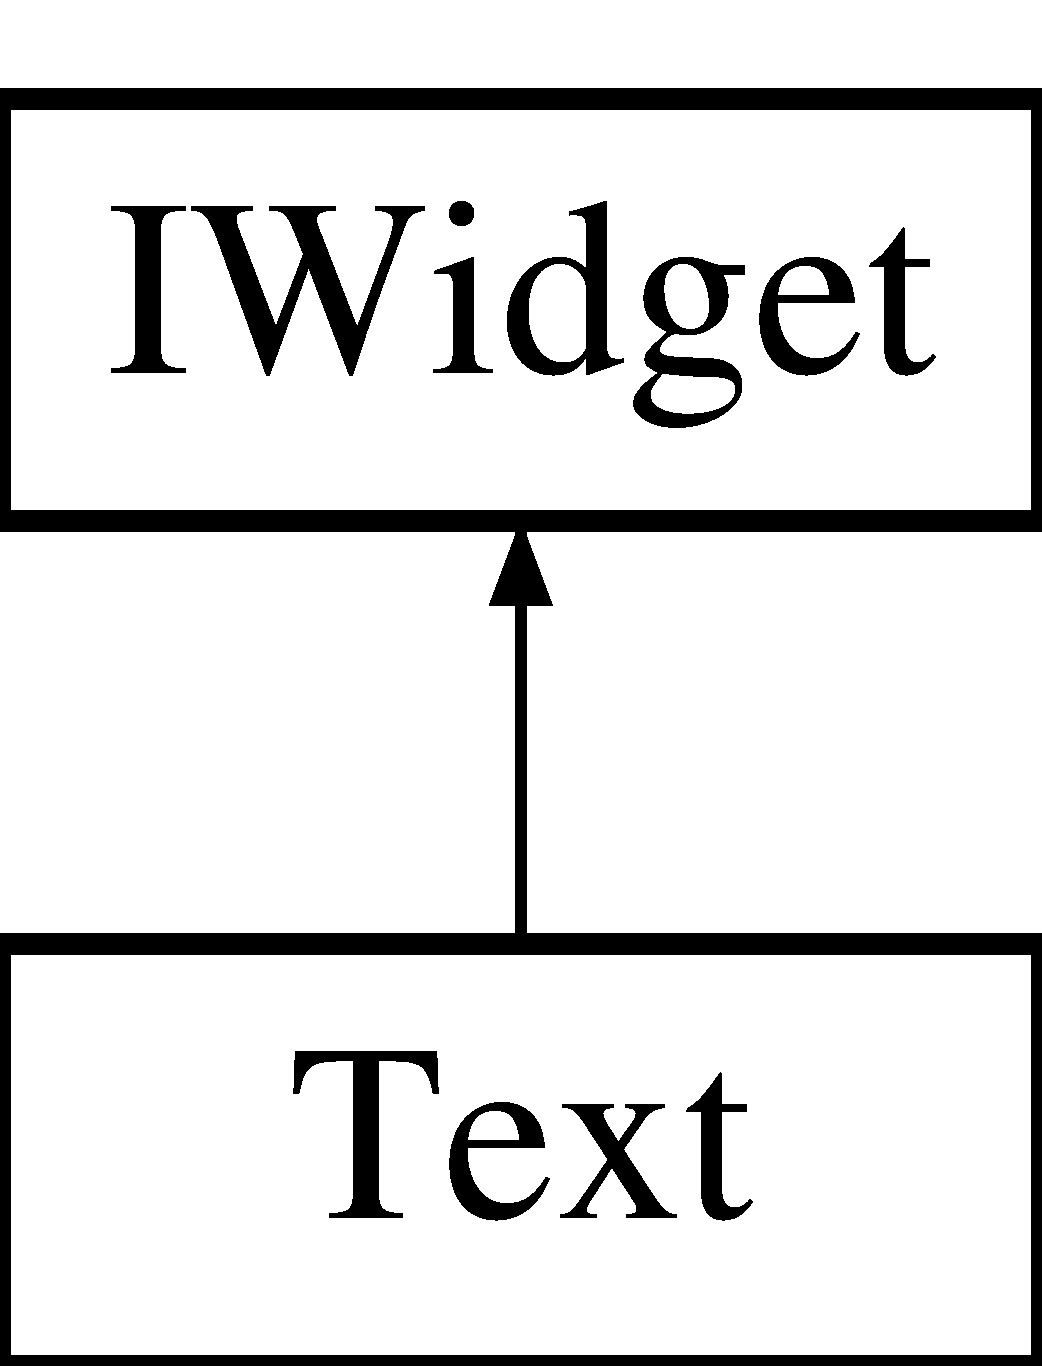
\includegraphics[height=2.000000cm]{classText}
\end{center}
\end{figure}
\subsection*{Public Member Functions}
\begin{DoxyCompactItemize}
\item 
\hyperlink{classText_a00ba9f4a2c3ca172e17433d2ceda4d55}{Text} (W\+String text, Rect pos, std\+::string font\+Name=\char`\"{}chow\+\_\+fun\char`\"{}, std\+::size\+\_\+t font\+Size=96)
\begin{DoxyCompactList}\small\item\em Constructor. \end{DoxyCompactList}\item 
void \hyperlink{classText_a811c378e24edd0a661cbc0e77ae4e785}{print} (\hyperlink{classWindow}{Window} $\ast$win)
\begin{DoxyCompactList}\small\item\em Display the text box on the screen. \end{DoxyCompactList}\end{DoxyCompactItemize}


\subsection{Detailed Description}
Inherited from a \hyperlink{classIWidget}{I\+Widget}. 

\subsection{Constructor \& Destructor Documentation}
\mbox{\Hypertarget{classText_a00ba9f4a2c3ca172e17433d2ceda4d55}\label{classText_a00ba9f4a2c3ca172e17433d2ceda4d55}} 
\index{Text@{Text}!Text@{Text}}
\index{Text@{Text}!Text@{Text}}
\subsubsection{\texorpdfstring{Text()}{Text()}}
{\footnotesize\ttfamily Text\+::\+Text (\begin{DoxyParamCaption}\item[{W\+String}]{text,  }\item[{Rect}]{pos,  }\item[{std\+::string}]{font\+Name = {\ttfamily \char`\"{}chow\+\_\+fun\char`\"{}},  }\item[{std\+::size\+\_\+t}]{font\+Size = {\ttfamily 96} }\end{DoxyParamCaption})}



Constructor. 


\begin{DoxyParams}{Parameters}
{\em text} & The data \\
\hline
{\em pos} & The position and the size of the text box \\
\hline
{\em font\+Name} & The font name to be used \\
\hline
{\em font\+Size} & The size of the font (8, 9, 10, 11, 12, 14, 18, 24, 30, 36, 48, 60, 72, 96) \\
\hline
\end{DoxyParams}


\subsection{Member Function Documentation}
\mbox{\Hypertarget{classText_a811c378e24edd0a661cbc0e77ae4e785}\label{classText_a811c378e24edd0a661cbc0e77ae4e785}} 
\index{Text@{Text}!print@{print}}
\index{print@{print}!Text@{Text}}
\subsubsection{\texorpdfstring{print()}{print()}}
{\footnotesize\ttfamily void Text\+::print (\begin{DoxyParamCaption}\item[{\hyperlink{classWindow}{Window} $\ast$}]{win }\end{DoxyParamCaption})\hspace{0.3cm}{\ttfamily [virtual]}}



Display the text box on the screen. 


\begin{DoxyParams}{Parameters}
{\em win} & The window \\
\hline
\end{DoxyParams}


Implements \hyperlink{classIWidget_a0cfa49a402e9bb31808a715e048ab2f4}{I\+Widget}.



The documentation for this class was generated from the following files\+:\begin{DoxyCompactItemize}
\item 
inc/graphics/widgets/\hyperlink{Text_8hh}{Text.\+hh}\item 
src/graphics/widgets/Text.\+cpp\end{DoxyCompactItemize}

\hypertarget{classWindow}{}\section{Window Class Reference}
\label{classWindow}\index{Window@{Window}}


Represent the window that will print some scene (view of the application).  




{\ttfamily \#include $<$Window.\+hh$>$}

\subsection*{Public Member Functions}
\begin{DoxyCompactItemize}
\item 
\hyperlink{classWindow_a25fd6af55e81b781b132166f77daf77e}{Window} (const wchar\+\_\+t $\ast$window\+Name)
\begin{DoxyCompactList}\small\item\em Constructor. \end{DoxyCompactList}\item 
\hyperlink{classWindow_a245d821e6016fa1f6970ccbbedd635f6}{$\sim$\+Window} ()
\begin{DoxyCompactList}\small\item\em Destructor. \end{DoxyCompactList}\item 
bool \hyperlink{classWindow_aa0dde1e5d56fd85fc1615bf34d67c9e0}{failed} () const
\begin{DoxyCompactList}\small\item\em Handle failed while building the window. \end{DoxyCompactList}\item 
void \hyperlink{classWindow_ac9150ac221e5569e677586d5a1123518}{add\+Scene} (const String \&name, const std\+::shared\+\_\+ptr$<$ \hyperlink{classAScene}{A\+Scene} $>$ \&scene)
\begin{DoxyCompactList}\small\item\em Allow the user to add a scene in the window. \end{DoxyCompactList}\item 
void \hyperlink{classWindow_a9e73c1dc8b22cdf16e6446af6f7ade48}{print\+Scene} (const String \&name)
\begin{DoxyCompactList}\small\item\em Allow the user to print a scene in the window. \end{DoxyCompactList}\item 
void \hyperlink{classWindow_ad3a1ead02eca314e2df94e3e932fb5ae}{delete\+Scene} (const String \&name)
\begin{DoxyCompactList}\small\item\em Allow the user ti delete a scene in the window. \end{DoxyCompactList}\item 
void \hyperlink{classWindow_a3342dc02339a5974d5c6fcefd91d0cbf}{set\+Current\+Scene} (const String \&scene\+Name)
\begin{DoxyCompactList}\small\item\em Set the current scene that will be print. \end{DoxyCompactList}\item 
void \hyperlink{classWindow_af1b2a635ce47d9e841445b8b866a3b28}{change\+Scene} ()
\begin{DoxyCompactList}\small\item\em Apply the set\+Current\+Scene\textquotesingle{}s changes. \end{DoxyCompactList}\item 
void \hyperlink{classWindow_a9c9f1fd6ebc2b93f16ca870487a4a4c6}{loop} (const String \&scene\+Name)
\begin{DoxyCompactList}\small\item\em Keep the window open util the end of the program\textquotesingle{}s execution. \end{DoxyCompactList}\end{DoxyCompactItemize}


\subsection{Detailed Description}
Represent the window that will print some scene (view of the application). 

\subsection{Constructor \& Destructor Documentation}
\mbox{\Hypertarget{classWindow_a25fd6af55e81b781b132166f77daf77e}\label{classWindow_a25fd6af55e81b781b132166f77daf77e}} 
\index{Window@{Window}!Window@{Window}}
\index{Window@{Window}!Window@{Window}}
\subsubsection{\texorpdfstring{Window()}{Window()}}
{\footnotesize\ttfamily Window\+::\+Window (\begin{DoxyParamCaption}\item[{const wchar\+\_\+t $\ast$}]{window\+Name }\end{DoxyParamCaption})}



Constructor. 

Build the class.


\begin{DoxyParams}{Parameters}
{\em \textquotesingle{}window\+Name\textquotesingle{}} & the window name that will be print on the top of the window. \\
\hline
\end{DoxyParams}
\mbox{\Hypertarget{classWindow_a245d821e6016fa1f6970ccbbedd635f6}\label{classWindow_a245d821e6016fa1f6970ccbbedd635f6}} 
\index{Window@{Window}!````~Window@{$\sim$\+Window}}
\index{````~Window@{$\sim$\+Window}!Window@{Window}}
\subsubsection{\texorpdfstring{$\sim$\+Window()}{~Window()}}
{\footnotesize\ttfamily Window\+::$\sim$\+Window (\begin{DoxyParamCaption}{ }\end{DoxyParamCaption})}



Destructor. 

Destroy the class. 

\subsection{Member Function Documentation}
\mbox{\Hypertarget{classWindow_ac9150ac221e5569e677586d5a1123518}\label{classWindow_ac9150ac221e5569e677586d5a1123518}} 
\index{Window@{Window}!add\+Scene@{add\+Scene}}
\index{add\+Scene@{add\+Scene}!Window@{Window}}
\subsubsection{\texorpdfstring{add\+Scene()}{addScene()}}
{\footnotesize\ttfamily void Window\+::add\+Scene (\begin{DoxyParamCaption}\item[{const String \&}]{name,  }\item[{const std\+::shared\+\_\+ptr$<$ \hyperlink{classAScene}{A\+Scene} $>$ \&}]{scene }\end{DoxyParamCaption})}



Allow the user to add a scene in the window. 


\begin{DoxyParams}{Parameters}
{\em 1)} & \textquotesingle{}name\textquotesingle{} of the scene that will be add. 2) \textquotesingle{}scene\textquotesingle{} a smart pointer on the scene that will be add. \\
\hline
\end{DoxyParams}
\mbox{\Hypertarget{classWindow_af1b2a635ce47d9e841445b8b866a3b28}\label{classWindow_af1b2a635ce47d9e841445b8b866a3b28}} 
\index{Window@{Window}!change\+Scene@{change\+Scene}}
\index{change\+Scene@{change\+Scene}!Window@{Window}}
\subsubsection{\texorpdfstring{change\+Scene()}{changeScene()}}
{\footnotesize\ttfamily void Window\+::change\+Scene (\begin{DoxyParamCaption}{ }\end{DoxyParamCaption})}



Apply the set\+Current\+Scene\textquotesingle{}s changes. 


\begin{DoxyParams}{Parameters}
{\em None.} & \\
\hline
\end{DoxyParams}
\mbox{\Hypertarget{classWindow_ad3a1ead02eca314e2df94e3e932fb5ae}\label{classWindow_ad3a1ead02eca314e2df94e3e932fb5ae}} 
\index{Window@{Window}!delete\+Scene@{delete\+Scene}}
\index{delete\+Scene@{delete\+Scene}!Window@{Window}}
\subsubsection{\texorpdfstring{delete\+Scene()}{deleteScene()}}
{\footnotesize\ttfamily void Window\+::delete\+Scene (\begin{DoxyParamCaption}\item[{const String \&}]{name }\end{DoxyParamCaption})}



Allow the user ti delete a scene in the window. 


\begin{DoxyParams}{Parameters}
{\em \textquotesingle{}name\textquotesingle{}} & the name of the scene that will be delete. \\
\hline
\end{DoxyParams}
\mbox{\Hypertarget{classWindow_aa0dde1e5d56fd85fc1615bf34d67c9e0}\label{classWindow_aa0dde1e5d56fd85fc1615bf34d67c9e0}} 
\index{Window@{Window}!failed@{failed}}
\index{failed@{failed}!Window@{Window}}
\subsubsection{\texorpdfstring{failed()}{failed()}}
{\footnotesize\ttfamily bool Window\+::failed (\begin{DoxyParamCaption}{ }\end{DoxyParamCaption}) const}



Handle failed while building the window. 


\begin{DoxyParams}{Parameters}
{\em None.} & \\
\hline
\end{DoxyParams}
\mbox{\Hypertarget{classWindow_a9c9f1fd6ebc2b93f16ca870487a4a4c6}\label{classWindow_a9c9f1fd6ebc2b93f16ca870487a4a4c6}} 
\index{Window@{Window}!loop@{loop}}
\index{loop@{loop}!Window@{Window}}
\subsubsection{\texorpdfstring{loop()}{loop()}}
{\footnotesize\ttfamily void Window\+::loop (\begin{DoxyParamCaption}\item[{const String \&}]{scene\+Name }\end{DoxyParamCaption})}



Keep the window open util the end of the program\textquotesingle{}s execution. 


\begin{DoxyParams}{Parameters}
{\em \textquotesingle{}scene\+Name\textquotesingle{}} & the scene\textquotesingle{}s name that will be launch at the begin of the program\textquotesingle{}s execution. \\
\hline
\end{DoxyParams}
\mbox{\Hypertarget{classWindow_a9e73c1dc8b22cdf16e6446af6f7ade48}\label{classWindow_a9e73c1dc8b22cdf16e6446af6f7ade48}} 
\index{Window@{Window}!print\+Scene@{print\+Scene}}
\index{print\+Scene@{print\+Scene}!Window@{Window}}
\subsubsection{\texorpdfstring{print\+Scene()}{printScene()}}
{\footnotesize\ttfamily void Window\+::print\+Scene (\begin{DoxyParamCaption}\item[{const String \&}]{name }\end{DoxyParamCaption})}



Allow the user to print a scene in the window. 


\begin{DoxyParams}{Parameters}
{\em \textquotesingle{}name\textquotesingle{}} & the name of the scene that will be print. \\
\hline
\end{DoxyParams}
\mbox{\Hypertarget{classWindow_a3342dc02339a5974d5c6fcefd91d0cbf}\label{classWindow_a3342dc02339a5974d5c6fcefd91d0cbf}} 
\index{Window@{Window}!set\+Current\+Scene@{set\+Current\+Scene}}
\index{set\+Current\+Scene@{set\+Current\+Scene}!Window@{Window}}
\subsubsection{\texorpdfstring{set\+Current\+Scene()}{setCurrentScene()}}
{\footnotesize\ttfamily void Window\+::set\+Current\+Scene (\begin{DoxyParamCaption}\item[{const String \&}]{scene\+Name }\end{DoxyParamCaption})}



Set the current scene that will be print. 


\begin{DoxyParams}{Parameters}
{\em \textquotesingle{}scene\+Name\textquotesingle{}} & the name of the scene that will be set as the current scene. \\
\hline
\end{DoxyParams}


The documentation for this class was generated from the following files\+:\begin{DoxyCompactItemize}
\item 
inc/graphics/\hyperlink{Window_8hh}{Window.\+hh}\item 
src/graphics/Window.\+cpp\end{DoxyCompactItemize}

\chapter{File Documentation}
\hypertarget{Controller_8hh}{}\section{inc/event/\+Controller.hh File Reference}
\label{Controller_8hh}\index{inc/event/\+Controller.\+hh@{inc/event/\+Controller.\+hh}}


Use to handle \hyperlink{classController}{Controller} Event.  


{\ttfamily \#include $<$irrlicht/irrlicht.\+h$>$}\newline
\subsection*{Classes}
\begin{DoxyCompactItemize}
\item 
class \hyperlink{classController}{Controller}
\begin{DoxyCompactList}\small\item\em Use to handle \hyperlink{classController}{Controller} Event. \end{DoxyCompactList}\end{DoxyCompactItemize}


\subsection{Detailed Description}
Use to handle \hyperlink{classController}{Controller} Event. 

\begin{DoxyAuthor}{Author}
Leo Paol, Charles Paulet 
\end{DoxyAuthor}
\begin{DoxyVersion}{Version}
2.\+0 
\end{DoxyVersion}

\hypertarget{Keyboard_8hh}{}\section{inc/event/\+Keyboard.hh File Reference}
\label{Keyboard_8hh}\index{inc/event/\+Keyboard.\+hh@{inc/event/\+Keyboard.\+hh}}


Use to handle keyboard event.  


{\ttfamily \#include $<$irrlicht/irrlicht.\+h$>$}\newline
{\ttfamily \#include \char`\"{}Event.\+hh\char`\"{}}\newline
{\ttfamily \#include \char`\"{}Control.\+hh\char`\"{}}\newline
\subsection*{Classes}
\begin{DoxyCompactItemize}
\item 
class \hyperlink{classKeyboard}{Keyboard}
\begin{DoxyCompactList}\small\item\em Handle client keyboard event. \end{DoxyCompactList}\end{DoxyCompactItemize}


\subsection{Detailed Description}
Use to handle keyboard event. 

\begin{DoxyAuthor}{Author}
Hugo Ailleres, Charles Paulet 
\end{DoxyAuthor}
\begin{DoxyVersion}{Version}
2.\+0 
\end{DoxyVersion}

\hypertarget{Exception_8hh}{}\section{inc/exception/\+Exception.hh File Reference}
\label{Exception_8hh}\index{inc/exception/\+Exception.\+hh@{inc/exception/\+Exception.\+hh}}


Exception class.  


{\ttfamily \#include $<$exception$>$}\newline
{\ttfamily \#include $<$string$>$}\newline
\subsection*{Classes}
\begin{DoxyCompactItemize}
\item 
class \hyperlink{classerror_1_1Exception}{error\+::\+Exception}
\begin{DoxyCompactList}\small\item\em This class allow to throw some execption and handle it finely. \end{DoxyCompactList}\end{DoxyCompactItemize}


\subsection{Detailed Description}
Exception class. 

\begin{DoxyAuthor}{Author}
Théophile Champion 
\end{DoxyAuthor}
\begin{DoxyVersion}{Version}
1.\+0 
\end{DoxyVersion}

\hypertarget{Game_8hh}{}\section{inc/game/\+Game.hh File Reference}
\label{Game_8hh}\index{inc/game/\+Game.\+hh@{inc/game/\+Game.\+hh}}


Contain all the information about the game.  


{\ttfamily \#include $<$memory$>$}\newline
{\ttfamily \#include \char`\"{}Level.\+hh\char`\"{}}\newline
\subsection*{Classes}
\begin{DoxyCompactItemize}
\item 
class \hyperlink{classGame}{Game}
\begin{DoxyCompactList}\small\item\em The \hyperlink{classGame}{Game} class. \end{DoxyCompactList}\end{DoxyCompactItemize}


\subsection{Detailed Description}
Contain all the information about the game. 

\begin{DoxyAuthor}{Author}
Théophile Champion 
\end{DoxyAuthor}
\begin{DoxyVersion}{Version}
1.\+0 
\end{DoxyVersion}

\hypertarget{Level_8hh}{}\section{inc/game/level/\+Level.hh File Reference}
\label{Level_8hh}\index{inc/game/level/\+Level.\+hh@{inc/game/level/\+Level.\+hh}}


Use to create a level of the game.  


{\ttfamily \#include $<$irrlicht/irrlicht.\+h$>$}\newline
{\ttfamily \#include $<$vector$>$}\newline
{\ttfamily \#include $<$memory$>$}\newline
{\ttfamily \#include $<$string$>$}\newline
{\ttfamily \#include \char`\"{}Map\+Factory.\+hh\char`\"{}}\newline
{\ttfamily \#include \char`\"{}Map.\+hh\char`\"{}}\newline
\subsection*{Classes}
\begin{DoxyCompactItemize}
\item 
class \hyperlink{classLevel}{Level}
\begin{DoxyCompactList}\small\item\em Represent a game\textquotesingle{}s level. \end{DoxyCompactList}\end{DoxyCompactItemize}


\subsection{Detailed Description}
Use to create a level of the game. 

\begin{DoxyAuthor}{Author}
Charles Paulet, Théophile Champion 
\end{DoxyAuthor}
\begin{DoxyVersion}{Version}
2.\+0 
\end{DoxyVersion}

\hypertarget{Map_8hh}{}\section{inc/game/level/\+Map.hh File Reference}
\label{Map_8hh}\index{inc/game/level/\+Map.\+hh@{inc/game/level/\+Map.\+hh}}


Defines the map that is related to a level. The process to create a map is relatively simple. First of all, you\textquotesingle{}ve got to load a map with \hyperlink{classMap_a37024e6d47ca10cf83a331635fe041b7}{Map\+::load\+Map()} In a second time, you\textquotesingle{}ve got to retrieve all the nodes with a triangle selector container (meta) with load\+Scene\+Nodes Then, you can create collision response thanks to these nodes by calling init\+Collision\+Response\+Animator() Finally, you can draw the map (that should be achieved with draw\+All() bugs\+: If meshs/models arent loading properly. Double check the paths in the .irr file.  


{\ttfamily \#include $<$iostream$>$}\newline
{\ttfamily \#include $<$string$>$}\newline
{\ttfamily \#include \char`\"{}graphics\+\_\+header.\+hh\char`\"{}}\newline
{\ttfamily \#include \char`\"{}I\+Widget.\+hh\char`\"{}}\newline
\subsection*{Classes}
\begin{DoxyCompactItemize}
\item 
class \hyperlink{classMap}{Map}
\begin{DoxyCompactList}\small\item\em Represent a level\textquotesingle{}s map. \end{DoxyCompactList}\end{DoxyCompactItemize}


\subsection{Detailed Description}
Defines the map that is related to a level. The process to create a map is relatively simple. First of all, you\textquotesingle{}ve got to load a map with \hyperlink{classMap_a37024e6d47ca10cf83a331635fe041b7}{Map\+::load\+Map()} In a second time, you\textquotesingle{}ve got to retrieve all the nodes with a triangle selector container (meta) with load\+Scene\+Nodes Then, you can create collision response thanks to these nodes by calling init\+Collision\+Response\+Animator() Finally, you can draw the map (that should be achieved with draw\+All() bugs\+: If meshs/models arent loading properly. Double check the paths in the .irr file. 

\begin{DoxyAuthor}{Author}
Charles Paulet 
\end{DoxyAuthor}
\begin{DoxyVersion}{Version}
0.\+1 
\end{DoxyVersion}

\hypertarget{MapFactory_8hh}{}\section{inc/game/level/\+Map\+Factory.hh File Reference}
\label{MapFactory_8hh}\index{inc/game/level/\+Map\+Factory.\+hh@{inc/game/level/\+Map\+Factory.\+hh}}


Maps\textquotesingle{} factory use to build the maps objects.  


{\ttfamily \#include $<$memory$>$}\newline
{\ttfamily \#include \char`\"{}Map.\+hh\char`\"{}}\newline
\subsection*{Classes}
\begin{DoxyCompactItemize}
\item 
class \hyperlink{classMapFactory}{Map\+Factory}
\begin{DoxyCompactList}\small\item\em Represent a maps\textquotesingle{} factory. \end{DoxyCompactList}\end{DoxyCompactItemize}


\subsection{Detailed Description}
Maps\textquotesingle{} factory use to build the maps objects. 

\begin{DoxyAuthor}{Author}
Charles Paulet 
\end{DoxyAuthor}
\begin{DoxyVersion}{Version}
0.\+1 
\end{DoxyVersion}

\hypertarget{AObject_8hh}{}\section{inc/game/object/\+A\+Object.hh File Reference}
\label{AObject_8hh}\index{inc/game/object/\+A\+Object.\+hh@{inc/game/object/\+A\+Object.\+hh}}


Use to create object.  


{\ttfamily \#include $<$irrlicht/irrlicht.\+h$>$}\newline
{\ttfamily \#include \char`\"{}Model3d.\+hh\char`\"{}}\newline
\subsection*{Classes}
\begin{DoxyCompactItemize}
\item 
class \hyperlink{classAObject}{A\+Object}
\begin{DoxyCompactList}\small\item\em An \hyperlink{classAObject}{A\+Object} instance has his own \hyperlink{classModel3d}{Model3d} attribute, and can modify it.. \end{DoxyCompactList}\end{DoxyCompactItemize}


\subsection{Detailed Description}
Use to create object. 

\begin{DoxyAuthor}{Author}
Hugo Ailleres 
\end{DoxyAuthor}
\begin{DoxyVersion}{Version}
1.\+0 
\end{DoxyVersion}

\hypertarget{APickable_8hh}{}\section{inc/game/object/\+A\+Pickable.hh File Reference}
\label{APickable_8hh}\index{inc/game/object/\+A\+Pickable.\+hh@{inc/game/object/\+A\+Pickable.\+hh}}


Use to create pickable object.  


{\ttfamily \#include \char`\"{}A\+Object.\+hh\char`\"{}}\newline
\subsection*{Classes}
\begin{DoxyCompactItemize}
\item 
class \hyperlink{classAPickable}{A\+Pickable}
\begin{DoxyCompactList}\small\item\em Create a pickable \hyperlink{classAObject}{A\+Object}. \end{DoxyCompactList}\end{DoxyCompactItemize}


\subsection{Detailed Description}
Use to create pickable object. 

\begin{DoxyAuthor}{Author}
Hugo Ailleres 
\end{DoxyAuthor}
\begin{DoxyVersion}{Version}
1.\+0 
\end{DoxyVersion}

\hypertarget{AScene_8hh}{}\section{inc/graphics/\+A\+Scene.hh File Reference}
\label{AScene_8hh}\index{inc/graphics/\+A\+Scene.\+hh@{inc/graphics/\+A\+Scene.\+hh}}


Define a window\textquotesingle{}s scene.  


{\ttfamily \#include $<$irrlicht/irrlicht.\+h$>$}\newline
{\ttfamily \#include $<$memory$>$}\newline
{\ttfamily \#include $<$vector$>$}\newline
\subsection*{Classes}
\begin{DoxyCompactItemize}
\item 
class \hyperlink{classAScene}{A\+Scene}
\begin{DoxyCompactList}\small\item\em Represent the window\textquotesingle{}s scene that will print some widget/object of the scene \+: buttons, images, etc... \end{DoxyCompactList}\end{DoxyCompactItemize}


\subsection{Detailed Description}
Define a window\textquotesingle{}s scene. 

\begin{DoxyAuthor}{Author}
Théophile Champion 
\end{DoxyAuthor}
\begin{DoxyVersion}{Version}
1.\+0 
\end{DoxyVersion}

\hypertarget{Camera_8hh}{}\section{inc/graphics/\+Camera.hh File Reference}
\label{Camera_8hh}\index{inc/graphics/\+Camera.\+hh@{inc/graphics/\+Camera.\+hh}}


Defines the camera, its type and behaviour  Actually you have to give the constructor the camera. That may change soon with integration on indie\+\_\+studio This way, cam will be created inside cosntructor with the g\+\_\+\+Window-\/$>$scene\+Manager that would be such accessible.  


\subsection*{Classes}
\begin{DoxyCompactItemize}
\item 
class \hyperlink{classCamera}{Camera}
\begin{DoxyCompactList}\small\item\em where cameras behaviour is defined \end{DoxyCompactList}\end{DoxyCompactItemize}


\subsection{Detailed Description}
Defines the camera, its type and behaviour  Actually you have to give the constructor the camera. That may change soon with integration on indie\+\_\+studio This way, cam will be created inside cosntructor with the g\+\_\+\+Window-\/$>$scene\+Manager that would be such accessible. 

\hyperlink{classCamera}{Camera} positionning may be set using Maths\+::get\+Centroid as position

\begin{DoxyAuthor}{Author}
Charles Paulet 
\end{DoxyAuthor}
\begin{DoxyVersion}{Version}
0.\+1 
\end{DoxyVersion}

\hypertarget{Gravity_8hh}{}\section{inc/graphics/\+Gravity.hh File Reference}
\label{Gravity_8hh}\index{inc/graphics/\+Gravity.\+hh@{inc/graphics/\+Gravity.\+hh}}


Define gravity for 3d models.  


{\ttfamily \#include \char`\"{}irrlicht/irrlicht.\+h\char`\"{}}\newline
{\ttfamily \#include \char`\"{}graphics\+\_\+header.\+hh\char`\"{}}\newline
{\ttfamily \#include \char`\"{}type\+\_\+compatibility.\+hh\char`\"{}}\newline
\subsection*{Classes}
\begin{DoxyCompactItemize}
\item 
class \hyperlink{classGravity}{Gravity}
\begin{DoxyCompactList}\small\item\em where \hyperlink{classGravity}{Gravity} behaviour is defined \end{DoxyCompactList}\end{DoxyCompactItemize}


\subsection{Detailed Description}
Define gravity for 3d models. 

\begin{DoxyAuthor}{Author}
Clovis Peridy, Charles Paulet 
\end{DoxyAuthor}
\begin{DoxyVersion}{Version}
2.\+0 
\end{DoxyVersion}

\hypertarget{GameMenuReceiver_8hh}{}\section{inc/graphics/scenes/events/\+Game\+Menu\+Receiver.hh File Reference}
\label{GameMenuReceiver_8hh}\index{inc/graphics/scenes/events/\+Game\+Menu\+Receiver.\+hh@{inc/graphics/scenes/events/\+Game\+Menu\+Receiver.\+hh}}


Use to manage event of the game (new game / load) scene.  


{\ttfamily \#include $<$irrlicht/irrlicht.\+h$>$}\newline
{\ttfamily \#include $<$memory$>$}\newline
{\ttfamily \#include \char`\"{}A\+Scene.\+hh\char`\"{}}\newline
\subsection*{Classes}
\begin{DoxyCompactItemize}
\item 
class \hyperlink{classGameMenuReceiver}{Game\+Menu\+Receiver}
\begin{DoxyCompactList}\small\item\em Manager of event of game scene. \end{DoxyCompactList}\end{DoxyCompactItemize}


\subsection{Detailed Description}
Use to manage event of the game (new game / load) scene. 

\begin{DoxyAuthor}{Author}
Leo P\+A\+OL 
\end{DoxyAuthor}
\begin{DoxyVersion}{Version}
1.\+0 
\end{DoxyVersion}

\hypertarget{GameNewReceiver_8hh}{}\section{inc/graphics/scenes/events/\+Game\+New\+Receiver.hh File Reference}
\label{GameNewReceiver_8hh}\index{inc/graphics/scenes/events/\+Game\+New\+Receiver.\+hh@{inc/graphics/scenes/events/\+Game\+New\+Receiver.\+hh}}


Use to manage event of the new game (character selection) scene.  


{\ttfamily \#include $<$irrlicht/irrlicht.\+h$>$}\newline
{\ttfamily \#include $<$memory$>$}\newline
{\ttfamily \#include \char`\"{}A\+Scene.\+hh\char`\"{}}\newline
\subsection*{Classes}
\begin{DoxyCompactItemize}
\item 
class \hyperlink{classGameNewReceiver}{Game\+New\+Receiver}
\begin{DoxyCompactList}\small\item\em Manager of event of new game scene. \end{DoxyCompactList}\end{DoxyCompactItemize}


\subsection{Detailed Description}
Use to manage event of the new game (character selection) scene. 

\begin{DoxyAuthor}{Author}
Leo P\+A\+OL 
\end{DoxyAuthor}
\begin{DoxyVersion}{Version}
1.\+0 
\end{DoxyVersion}

\hypertarget{OptionSoundReceiver_8hh}{}\section{inc/graphics/scenes/events/\+Option\+Sound\+Receiver.hh File Reference}
\label{OptionSoundReceiver_8hh}\index{inc/graphics/scenes/events/\+Option\+Sound\+Receiver.\+hh@{inc/graphics/scenes/events/\+Option\+Sound\+Receiver.\+hh}}


Allow to manage event of Sound scene setting.  


{\ttfamily \#include $<$irrlicht/irrlicht.\+h$>$}\newline
{\ttfamily \#include $<$memory$>$}\newline
{\ttfamily \#include \char`\"{}A\+Scene.\+hh\char`\"{}}\newline
\subsection*{Classes}
\begin{DoxyCompactItemize}
\item 
class \hyperlink{classOptionSoundReceiver}{Option\+Sound\+Receiver}
\begin{DoxyCompactList}\small\item\em Manager of event of Sound scene setting. \end{DoxyCompactList}\end{DoxyCompactItemize}


\subsection{Detailed Description}
Allow to manage event of Sound scene setting. 

\begin{DoxyAuthor}{Author}
Hugo Ailleres 
\end{DoxyAuthor}
\begin{DoxyVersion}{Version}
1.\+0 
\end{DoxyVersion}

\hypertarget{OptionVideoReceiver_8hh}{}\section{inc/graphics/scenes/events/\+Option\+Video\+Receiver.hh File Reference}
\label{OptionVideoReceiver_8hh}\index{inc/graphics/scenes/events/\+Option\+Video\+Receiver.\+hh@{inc/graphics/scenes/events/\+Option\+Video\+Receiver.\+hh}}


Use to manage event of the video setting scene.  


{\ttfamily \#include $<$irrlicht/irrlicht.\+h$>$}\newline
{\ttfamily \#include $<$memory$>$}\newline
{\ttfamily \#include \char`\"{}A\+Scene.\+hh\char`\"{}}\newline
\subsection*{Classes}
\begin{DoxyCompactItemize}
\item 
class \hyperlink{classOptionVideoReceiver}{Option\+Video\+Receiver}
\begin{DoxyCompactList}\small\item\em Manager of event of video setting scene. \end{DoxyCompactList}\end{DoxyCompactItemize}


\subsection{Detailed Description}
Use to manage event of the video setting scene. 

\begin{DoxyAuthor}{Author}
Leo P\+A\+OL 
\end{DoxyAuthor}
\begin{DoxyVersion}{Version}
1.\+0 
\end{DoxyVersion}

\hypertarget{GameLoadScene_8hh}{}\section{inc/graphics/scenes/\+Game\+Load\+Scene.hh File Reference}
\label{GameLoadScene_8hh}\index{inc/graphics/scenes/\+Game\+Load\+Scene.\+hh@{inc/graphics/scenes/\+Game\+Load\+Scene.\+hh}}


Use to display the gameload scene.  


{\ttfamily \#include $<$irrlicht/irrlicht.\+h$>$}\newline
{\ttfamily \#include $<$memory$>$}\newline
{\ttfamily \#include \char`\"{}graphics\+\_\+header.\+hh\char`\"{}}\newline
\subsection*{Classes}
\begin{DoxyCompactItemize}
\item 
class \hyperlink{classGameLoadScene}{Game\+Load\+Scene}
\begin{DoxyCompactList}\small\item\em \hyperlink{classButton}{Button} interface of Game\+Load scene. \end{DoxyCompactList}\end{DoxyCompactItemize}


\subsection{Detailed Description}
Use to display the gameload scene. 

\begin{DoxyAuthor}{Author}
Clovis Peridy 
\end{DoxyAuthor}
\begin{DoxyVersion}{Version}
1.\+0 
\end{DoxyVersion}

\hypertarget{GameMenuScene_8hh}{}\section{inc/graphics/scenes/\+Game\+Menu\+Scene.hh File Reference}
\label{GameMenuScene_8hh}\index{inc/graphics/scenes/\+Game\+Menu\+Scene.\+hh@{inc/graphics/scenes/\+Game\+Menu\+Scene.\+hh}}


Use to choose between new game and load game.  


{\ttfamily \#include $<$irrlicht/irrlicht.\+h$>$}\newline
{\ttfamily \#include $<$memory$>$}\newline
{\ttfamily \#include \char`\"{}graphics\+\_\+header.\+hh\char`\"{}}\newline
\subsection*{Classes}
\begin{DoxyCompactItemize}
\item 
class \hyperlink{classGameMenuScene}{Game\+Menu\+Scene}
\begin{DoxyCompactList}\small\item\em \hyperlink{classButton}{Button} interface of menu setting scene. \end{DoxyCompactList}\end{DoxyCompactItemize}


\subsection{Detailed Description}
Use to choose between new game and load game. 

\begin{DoxyAuthor}{Author}
Leo P\+A\+OL 
\end{DoxyAuthor}
\begin{DoxyVersion}{Version}
1.\+0 
\end{DoxyVersion}

\hypertarget{GameNewScene_8hh}{}\section{inc/graphics/scenes/\+Game\+New\+Scene.hh File Reference}
\label{GameNewScene_8hh}\index{inc/graphics/scenes/\+Game\+New\+Scene.\+hh@{inc/graphics/scenes/\+Game\+New\+Scene.\+hh}}


Use to choose characters for each player.  


{\ttfamily \#include $<$irrlicht/irrlicht.\+h$>$}\newline
{\ttfamily \#include $<$memory$>$}\newline
{\ttfamily \#include \char`\"{}graphics\+\_\+header.\+hh\char`\"{}}\newline
\subsection*{Classes}
\begin{DoxyCompactItemize}
\item 
class \hyperlink{classGameNewScene}{Game\+New\+Scene}
\begin{DoxyCompactList}\small\item\em \hyperlink{classButton}{Button} interface of new game setting scene. \end{DoxyCompactList}\end{DoxyCompactItemize}


\subsection{Detailed Description}
Use to choose characters for each player. 

\begin{DoxyAuthor}{Author}
Leo P\+A\+OL 
\end{DoxyAuthor}
\begin{DoxyVersion}{Version}
1.\+0 
\end{DoxyVersion}

\hypertarget{GameOnlineScene_8hh}{}\section{inc/graphics/scenes/\+Game\+Online\+Scene.hh File Reference}
\label{GameOnlineScene_8hh}\index{inc/graphics/scenes/\+Game\+Online\+Scene.\+hh@{inc/graphics/scenes/\+Game\+Online\+Scene.\+hh}}


Use to display the Game\+Online scene.  


{\ttfamily \#include $<$irrlicht/irrlicht.\+h$>$}\newline
{\ttfamily \#include $<$memory$>$}\newline
{\ttfamily \#include \char`\"{}graphics\+\_\+header.\+hh\char`\"{}}\newline
\subsection*{Classes}
\begin{DoxyCompactItemize}
\item 
class \hyperlink{classGameOnlineScene}{Game\+Online\+Scene}
\begin{DoxyCompactList}\small\item\em \hyperlink{classButton}{Button} interface of Game\+Onlinescene. \end{DoxyCompactList}\end{DoxyCompactItemize}


\subsection{Detailed Description}
Use to display the Game\+Online scene. 

\begin{DoxyAuthor}{Author}
Clovis Peridy 
\end{DoxyAuthor}
\begin{DoxyVersion}{Version}
1.\+0 
\end{DoxyVersion}

\hypertarget{GameScene_8hh}{}\section{inc/graphics/scenes/\+Game\+Scene.hh File Reference}
\label{GameScene_8hh}\index{inc/graphics/scenes/\+Game\+Scene.\+hh@{inc/graphics/scenes/\+Game\+Scene.\+hh}}


Use to display the \hyperlink{classGame}{Game} scene.  


{\ttfamily \#include $<$irrlicht/irrlicht.\+h$>$}\newline
{\ttfamily \#include $<$memory$>$}\newline
{\ttfamily \#include \char`\"{}graphics\+\_\+header.\+hh\char`\"{}}\newline


\subsection{Detailed Description}
Use to display the \hyperlink{classGame}{Game} scene. 

\begin{DoxyAuthor}{Author}
Clovis Peridy 
\end{DoxyAuthor}
\begin{DoxyVersion}{Version}
1.\+0 
\end{DoxyVersion}

\hypertarget{GameSimulationScene_8hh}{}\section{inc/graphics/scenes/\+Game\+Simulation\+Scene.hh File Reference}
\label{GameSimulationScene_8hh}\index{inc/graphics/scenes/\+Game\+Simulation\+Scene.\+hh@{inc/graphics/scenes/\+Game\+Simulation\+Scene.\+hh}}


Use to display the Game\+Online scene.  


{\ttfamily \#include $<$irrlicht/irrlicht.\+h$>$}\newline
{\ttfamily \#include $<$memory$>$}\newline
{\ttfamily \#include \char`\"{}graphics\+\_\+header.\+hh\char`\"{}}\newline
\subsection*{Classes}
\begin{DoxyCompactItemize}
\item 
class \hyperlink{classGameSimulationScene}{Game\+Simulation\+Scene}
\begin{DoxyCompactList}\small\item\em \hyperlink{classButton}{Button} interface of Game\+Simulationscene. \end{DoxyCompactList}\end{DoxyCompactItemize}


\subsection{Detailed Description}
Use to display the Game\+Online scene. 

\begin{DoxyAuthor}{Author}
Clovis Peridy, Charles Paulet 
\end{DoxyAuthor}
\begin{DoxyVersion}{Version}
2.\+0 
\end{DoxyVersion}

\hypertarget{IntroScene_8hh}{}\section{inc/graphics/scenes/\+Intro\+Scene.hh File Reference}
\label{IntroScene_8hh}\index{inc/graphics/scenes/\+Intro\+Scene.\+hh@{inc/graphics/scenes/\+Intro\+Scene.\+hh}}


Use to display the \hyperlink{classIntroScene}{Intro\+Scene} scene.  


{\ttfamily \#include $<$irrlicht/irrlicht.\+h$>$}\newline
{\ttfamily \#include $<$memory$>$}\newline
{\ttfamily \#include \char`\"{}type\+\_\+compatibility.\+hh\char`\"{}}\newline
{\ttfamily \#include \char`\"{}graphics\+\_\+header.\+hh\char`\"{}}\newline
\subsection*{Classes}
\begin{DoxyCompactItemize}
\item 
class \hyperlink{classIntroScene}{Intro\+Scene}
\begin{DoxyCompactList}\small\item\em \hyperlink{classButton}{Button} interface of Introcene. \end{DoxyCompactList}\end{DoxyCompactItemize}


\subsection{Detailed Description}
Use to display the \hyperlink{classIntroScene}{Intro\+Scene} scene. 

\begin{DoxyAuthor}{Author}
Clovis Peridy 
\end{DoxyAuthor}
\begin{DoxyVersion}{Version}
1.\+0 
\end{DoxyVersion}

\hypertarget{LegendScene_8hh}{}\section{inc/graphics/scenes/\+Legend\+Scene.hh File Reference}
\label{LegendScene_8hh}\index{inc/graphics/scenes/\+Legend\+Scene.\+hh@{inc/graphics/scenes/\+Legend\+Scene.\+hh}}


Use to display the Legend scene.  


{\ttfamily \#include $<$irrlicht/irrlicht.\+h$>$}\newline
{\ttfamily \#include $<$memory$>$}\newline
{\ttfamily \#include \char`\"{}graphics\+\_\+header.\+hh\char`\"{}}\newline
\subsection*{Classes}
\begin{DoxyCompactItemize}
\item 
class \hyperlink{classLegendScene}{Legend\+Scene}
\begin{DoxyCompactList}\small\item\em \hyperlink{classButton}{Button} interface of \hyperlink{classLegendScene}{Legend\+Scene}. \end{DoxyCompactList}\end{DoxyCompactItemize}


\subsection{Detailed Description}
Use to display the Legend scene. 

\begin{DoxyAuthor}{Author}
Clovis Peridy 
\end{DoxyAuthor}
\begin{DoxyVersion}{Version}
1.\+0 
\end{DoxyVersion}

\hypertarget{MainScene_8hh}{}\section{inc/graphics/scenes/\+Main\+Scene.hh File Reference}
\label{MainScene_8hh}\index{inc/graphics/scenes/\+Main\+Scene.\+hh@{inc/graphics/scenes/\+Main\+Scene.\+hh}}


Main scene who lead to each menus.  


{\ttfamily \#include $<$irrlicht/irrlicht.\+h$>$}\newline
{\ttfamily \#include $<$memory$>$}\newline
{\ttfamily \#include \char`\"{}graphics\+\_\+header.\+hh\char`\"{}}\newline
\subsection*{Classes}
\begin{DoxyCompactItemize}
\item 
class \hyperlink{classMainScene}{Main\+Scene}
\begin{DoxyCompactList}\small\item\em \hyperlink{classButton}{Button} interface of main scene. \end{DoxyCompactList}\end{DoxyCompactItemize}


\subsection{Detailed Description}
Main scene who lead to each menus. 

\begin{DoxyAuthor}{Author}
Clovis Peridy 
\end{DoxyAuthor}
\begin{DoxyVersion}{Version}
1.\+0 
\end{DoxyVersion}

\hypertarget{OptionControlScene_8hh}{}\section{inc/graphics/scenes/\+Option\+Control\+Scene.hh File Reference}
\label{OptionControlScene_8hh}\index{inc/graphics/scenes/\+Option\+Control\+Scene.\+hh@{inc/graphics/scenes/\+Option\+Control\+Scene.\+hh}}


Use to display the \hyperlink{classOptionControl}{Option\+Control} scene.  


{\ttfamily \#include $<$irrlicht/irrlicht.\+h$>$}\newline
{\ttfamily \#include $<$memory$>$}\newline
{\ttfamily \#include \char`\"{}graphics\+\_\+header.\+hh\char`\"{}}\newline


\subsection{Detailed Description}
Use to display the \hyperlink{classOptionControl}{Option\+Control} scene. 

\begin{DoxyAuthor}{Author}
Clovis Peridy 
\end{DoxyAuthor}
\begin{DoxyVersion}{Version}
1.\+0 
\end{DoxyVersion}

\hypertarget{OptionScene_8hh}{}\section{inc/graphics/scenes/\+Option\+Scene.hh File Reference}
\label{OptionScene_8hh}\index{inc/graphics/scenes/\+Option\+Scene.\+hh@{inc/graphics/scenes/\+Option\+Scene.\+hh}}


Use to display the option menu.  


{\ttfamily \#include $<$irrlicht/irrlicht.\+h$>$}\newline
{\ttfamily \#include $<$memory$>$}\newline
{\ttfamily \#include \char`\"{}graphics\+\_\+header.\+hh\char`\"{}}\newline
\subsection*{Classes}
\begin{DoxyCompactItemize}
\item 
class \hyperlink{classOptionScene}{Option\+Scene}
\begin{DoxyCompactList}\small\item\em \hyperlink{classButton}{Button} interface of option scene. \end{DoxyCompactList}\end{DoxyCompactItemize}


\subsection{Detailed Description}
Use to display the option menu. 

\begin{DoxyAuthor}{Author}
Clovis Peridy 
\end{DoxyAuthor}
\begin{DoxyVersion}{Version}
1.\+0 
\end{DoxyVersion}

\hypertarget{OptionSoundScene_8hh}{}\section{inc/graphics/scenes/\+Option\+Sound\+Scene.hh File Reference}
\label{OptionSoundScene_8hh}\index{inc/graphics/scenes/\+Option\+Sound\+Scene.\+hh@{inc/graphics/scenes/\+Option\+Sound\+Scene.\+hh}}


Use to create the button interface of the sound setting scene.  


{\ttfamily \#include $<$irrlicht/irrlicht.\+h$>$}\newline
{\ttfamily \#include $<$memory$>$}\newline
{\ttfamily \#include \char`\"{}graphics\+\_\+header.\+hh\char`\"{}}\newline
\subsection*{Classes}
\begin{DoxyCompactItemize}
\item 
class \hyperlink{classOptionSoundScene}{Option\+Sound\+Scene}
\begin{DoxyCompactList}\small\item\em \hyperlink{classButton}{Button} interface of sound setting scene. \end{DoxyCompactList}\end{DoxyCompactItemize}


\subsection{Detailed Description}
Use to create the button interface of the sound setting scene. 

\begin{DoxyAuthor}{Author}
Hugo Ailleres 
\end{DoxyAuthor}
\begin{DoxyVersion}{Version}
1.\+0 
\end{DoxyVersion}

\hypertarget{OptionVideoScene_8hh}{}\section{inc/graphics/scenes/\+Option\+Video\+Scene.hh File Reference}
\label{OptionVideoScene_8hh}\index{inc/graphics/scenes/\+Option\+Video\+Scene.\+hh@{inc/graphics/scenes/\+Option\+Video\+Scene.\+hh}}


Use to create the button interface of the video setting scene.  


{\ttfamily \#include $<$irrlicht/irrlicht.\+h$>$}\newline
{\ttfamily \#include $<$memory$>$}\newline
{\ttfamily \#include \char`\"{}graphics\+\_\+header.\+hh\char`\"{}}\newline
\subsection*{Classes}
\begin{DoxyCompactItemize}
\item 
class \hyperlink{classOptionVideoScene}{Option\+Video\+Scene}
\begin{DoxyCompactList}\small\item\em \hyperlink{classButton}{Button} interface of video setting scene. \end{DoxyCompactList}\end{DoxyCompactItemize}


\subsection{Detailed Description}
Use to create the button interface of the video setting scene. 

\begin{DoxyAuthor}{Author}
Leo P\+A\+OL 
\end{DoxyAuthor}
\begin{DoxyVersion}{Version}
1.\+0 
\end{DoxyVersion}

\hypertarget{ScoreScene_8hh}{}\section{inc/graphics/scenes/\+Score\+Scene.hh File Reference}
\label{ScoreScene_8hh}\index{inc/graphics/scenes/\+Score\+Scene.\+hh@{inc/graphics/scenes/\+Score\+Scene.\+hh}}


Use to display the Score scene.  


{\ttfamily \#include $<$irrlicht/irrlicht.\+h$>$}\newline
{\ttfamily \#include $<$memory$>$}\newline
{\ttfamily \#include \char`\"{}Score\+Manager.\+hh\char`\"{}}\newline
{\ttfamily \#include \char`\"{}graphics\+\_\+header.\+hh\char`\"{}}\newline
{\ttfamily \#include \char`\"{}Text.\+hh\char`\"{}}\newline
\subsection*{Classes}
\begin{DoxyCompactItemize}
\item 
class \hyperlink{classScoreScene}{Score\+Scene}
\begin{DoxyCompactList}\small\item\em \hyperlink{classButton}{Button} interface of \hyperlink{classScoreScene}{Score\+Scene}. \end{DoxyCompactList}\end{DoxyCompactItemize}


\subsection{Detailed Description}
Use to display the Score scene. 

\begin{DoxyAuthor}{Author}
Clovis Peridy 
\end{DoxyAuthor}
\begin{DoxyVersion}{Version}
1.\+0 
\end{DoxyVersion}

\hypertarget{Button_8hh}{}\section{inc/graphics/widgets/\+Button.hh File Reference}
\label{Button_8hh}\index{inc/graphics/widgets/\+Button.\+hh@{inc/graphics/widgets/\+Button.\+hh}}


Allow to add some button in the window.  


{\ttfamily \#include \char`\"{}type\+\_\+compatibility.\+hh\char`\"{}}\newline
{\ttfamily \#include \char`\"{}graphics\+\_\+header.\+hh\char`\"{}}\newline
{\ttfamily \#include \char`\"{}G\+U\+I\+Button\+Id.\+hh\char`\"{}}\newline
\subsection*{Classes}
\begin{DoxyCompactItemize}
\item 
class \hyperlink{classButton}{Button}
\begin{DoxyCompactList}\small\item\em Represent a button in the user interface. \end{DoxyCompactList}\end{DoxyCompactItemize}


\subsection{Detailed Description}
Allow to add some button in the window. 

\begin{DoxyAuthor}{Author}
Théophile Champion, Charles Paulet 
\end{DoxyAuthor}
\begin{DoxyVersion}{Version}
4.\+0 
\end{DoxyVersion}

\hypertarget{Image_8hh}{}\section{inc/graphics/widgets/\+Image.hh File Reference}
\label{Image_8hh}\index{inc/graphics/widgets/\+Image.\+hh@{inc/graphics/widgets/\+Image.\+hh}}


Allow to add some image in the window.  


{\ttfamily \#include $<$irrlicht/irrlicht.\+h$>$}\newline
{\ttfamily \#include \char`\"{}type\+\_\+compatibility.\+hh\char`\"{}}\newline
{\ttfamily \#include \char`\"{}graphics\+\_\+header.\+hh\char`\"{}}\newline
\subsection*{Classes}
\begin{DoxyCompactItemize}
\item 
class \hyperlink{classImage}{Image}
\begin{DoxyCompactList}\small\item\em Represent a image in the user interface. \end{DoxyCompactList}\end{DoxyCompactItemize}


\subsection{Detailed Description}
Allow to add some image in the window. 

\begin{DoxyAuthor}{Author}
Théophile Champion 
\end{DoxyAuthor}
\begin{DoxyVersion}{Version}
1.\+0 
\end{DoxyVersion}

\hypertarget{IWidget_8hh}{}\section{inc/graphics/widgets/\+I\+Widget.hh File Reference}
\label{IWidget_8hh}\index{inc/graphics/widgets/\+I\+Widget.\+hh@{inc/graphics/widgets/\+I\+Widget.\+hh}}


Give a interface for all the class that could be print on the window.  


{\ttfamily \#include \char`\"{}graphics\+\_\+header.\+hh\char`\"{}}\newline
\subsection*{Classes}
\begin{DoxyCompactItemize}
\item 
class \hyperlink{classIWidget}{I\+Widget}
\begin{DoxyCompactList}\small\item\em Represent a generic object in the user interface. \end{DoxyCompactList}\end{DoxyCompactItemize}


\subsection{Detailed Description}
Give a interface for all the class that could be print on the window. 

\begin{DoxyAuthor}{Author}
Théophile Champion, Charles Paulet 
\end{DoxyAuthor}
\begin{DoxyVersion}{Version}
2.\+0 
\end{DoxyVersion}

\hypertarget{Model3d_8hh}{}\section{inc/graphics/widgets/\+Model3d.hh File Reference}
\label{Model3d_8hh}\index{inc/graphics/widgets/\+Model3d.\+hh@{inc/graphics/widgets/\+Model3d.\+hh}}


Allow to add some model 3d in the window.  


{\ttfamily \#include $<$iostream$>$}\newline
{\ttfamily \#include $<$vector$>$}\newline
{\ttfamily \#include $<$string$>$}\newline
{\ttfamily \#include $<$memory$>$}\newline
{\ttfamily \#include \char`\"{}type\+\_\+compatibility.\+hh\char`\"{}}\newline
{\ttfamily \#include \char`\"{}graphics\+\_\+header.\+hh\char`\"{}}\newline
{\ttfamily \#include \char`\"{}animation\+\_\+type.\+hh\char`\"{}}\newline
{\ttfamily \#include \char`\"{}Model.\+hh\char`\"{}}\newline
\subsection*{Classes}
\begin{DoxyCompactItemize}
\item 
class \hyperlink{classModel3d}{Model3d}
\begin{DoxyCompactList}\small\item\em Represent a model 3d in the user interface. \end{DoxyCompactList}\item 
struct \hyperlink{structModel3d_1_1AnimationSetting}{Model3d\+::\+Animation\+Setting}
\begin{DoxyCompactList}\small\item\em Represent a model\textquotesingle{}s animation\textquotesingle{}s setting. \end{DoxyCompactList}\end{DoxyCompactItemize}


\subsection{Detailed Description}
Allow to add some model 3d in the window. 

\begin{DoxyAuthor}{Author}
Théophile Champion, Charles Paulet 
\end{DoxyAuthor}
\begin{DoxyVersion}{Version}
2.\+0 
\end{DoxyVersion}

\hypertarget{Text_8hh}{}\section{inc/graphics/widgets/\+Text.hh File Reference}
\label{Text_8hh}\index{inc/graphics/widgets/\+Text.\+hh@{inc/graphics/widgets/\+Text.\+hh}}


Allow you to create a text object.  


{\ttfamily \#include \char`\"{}type\+\_\+compatibility.\+hh\char`\"{}}\newline
{\ttfamily \#include \char`\"{}graphics\+\_\+header.\+hh\char`\"{}}\newline
{\ttfamily \#include \char`\"{}G\+U\+I\+Button\+Id.\+hh\char`\"{}}\newline
{\ttfamily \#include \char`\"{}I\+Widget.\+hh\char`\"{}}\newline
{\ttfamily \#include \char`\"{}Core\+Manager.\+hh\char`\"{}}\newline
\subsection*{Classes}
\begin{DoxyCompactItemize}
\item 
class \hyperlink{classText}{Text}
\begin{DoxyCompactList}\small\item\em Inherited from a \hyperlink{classIWidget}{I\+Widget}. \end{DoxyCompactList}\end{DoxyCompactItemize}


\subsection{Detailed Description}
Allow you to create a text object. 

\begin{DoxyAuthor}{Author}
Nicolas-\/\+Emmanuel Robert 
\end{DoxyAuthor}
\begin{DoxyVersion}{Version}
1.\+0 
\end{DoxyVersion}

\hypertarget{Window_8hh}{}\section{inc/graphics/\+Window.hh File Reference}
\label{Window_8hh}\index{inc/graphics/\+Window.\+hh@{inc/graphics/\+Window.\+hh}}


Define a window.  


{\ttfamily \#include $<$irrlicht/irrlicht.\+h$>$}\newline
{\ttfamily \#include $<$memory$>$}\newline
{\ttfamily \#include $<$string$>$}\newline
{\ttfamily \#include $<$vector$>$}\newline
{\ttfamily \#include \char`\"{}type\+\_\+compatibility.\+hh\char`\"{}}\newline
{\ttfamily \#include \char`\"{}Core\+Manager.\+hh\char`\"{}}\newline
{\ttfamily \#include \char`\"{}Camera.\+hh\char`\"{}}\newline
{\ttfamily \#include \char`\"{}Cursor.\+hh\char`\"{}}\newline
{\ttfamily \#include \char`\"{}thread.\+hh\char`\"{}}\newline
\subsection*{Classes}
\begin{DoxyCompactItemize}
\item 
class \hyperlink{classWindow}{Window}
\begin{DoxyCompactList}\small\item\em Represent the window that will print some scene (view of the application). \end{DoxyCompactList}\end{DoxyCompactItemize}


\subsection{Detailed Description}
Define a window. 

\begin{DoxyAuthor}{Author}
Théophile Champion, Charles Paulet 
\end{DoxyAuthor}
\begin{DoxyVersion}{Version}
2.\+0 
\end{DoxyVersion}

\hypertarget{Control_8hh}{}\section{inc/managers/config/\+Control.hh File Reference}
\label{Control_8hh}\index{inc/managers/config/\+Control.\+hh@{inc/managers/config/\+Control.\+hh}}


Configuration for player\textquotesingle{}s keyboard.  


{\ttfamily \#include $<$string$>$}\newline
{\ttfamily \#include $<$utility$>$}\newline
{\ttfamily \#include $<$irrlicht/irrlicht.\+h$>$}\newline
\subsection*{Classes}
\begin{DoxyCompactItemize}
\item 
struct \hyperlink{structconfig_1_1ControlPlayer}{config\+::\+Control\+Player}
\begin{DoxyCompactList}\small\item\em This structure contain all the key that are necessary to a player. \end{DoxyCompactList}\item 
struct \hyperlink{structconfig_1_1Control}{config\+::\+Control}
\begin{DoxyCompactList}\small\item\em This structure contain two \hyperlink{structconfig_1_1ControlPlayer}{Control\+Player} structure (one for each player) \end{DoxyCompactList}\end{DoxyCompactItemize}


\subsection{Detailed Description}
Configuration for player\textquotesingle{}s keyboard. 

\begin{DoxyAuthor}{Author}
Nicolas-\/\+Emmanuel Robert 
\end{DoxyAuthor}
\begin{DoxyVersion}{Version}
1.\+0 
\end{DoxyVersion}

\hypertarget{Model_8hh}{}\section{inc/managers/config/\+Model.hh File Reference}
\label{Model_8hh}\index{inc/managers/config/\+Model.\+hh@{inc/managers/config/\+Model.\+hh}}


The Class Model allow you to manipulate model\textquotesingle{}s informations.  


{\ttfamily \#include $<$vector$>$}\newline
{\ttfamily \#include \char`\"{}type\+\_\+compatibility.\+hh\char`\"{}}\newline


\subsection{Detailed Description}
The Class Model allow you to manipulate model\textquotesingle{}s informations. 

The Class Video allow you to manipulate video\textquotesingle{}s configuration.

The Class Sound allow you to manipulate sound\textquotesingle{}s configuration.

The Class Score allow you to manipulate score\textquotesingle{}s informations.

\begin{DoxyAuthor}{Author}
Nicolas-\/\+Emmanuel Robert 
\end{DoxyAuthor}
\begin{DoxyVersion}{Version}
1.\+0 
\end{DoxyVersion}

\hypertarget{ConfigManager_8hh}{}\section{inc/managers/\+Config\+Manager.hh File Reference}
\label{ConfigManager_8hh}\index{inc/managers/\+Config\+Manager.\+hh@{inc/managers/\+Config\+Manager.\+hh}}


Allow you to load, modify and save the configuration.  


{\ttfamily \#include $<$irrlicht/irrlicht.\+h$>$}\newline
{\ttfamily \#include $<$irrlicht/irr\+X\+M\+L.\+h$>$}\newline
{\ttfamily \#include $<$iostream$>$}\newline
{\ttfamily \#include $<$fstream$>$}\newline
{\ttfamily \#include $<$string$>$}\newline
{\ttfamily \#include $<$vector$>$}\newline
{\ttfamily \#include $<$map$>$}\newline
{\ttfamily \#include \char`\"{}Control.\+hh\char`\"{}}\newline
{\ttfamily \#include \char`\"{}Video.\+hh\char`\"{}}\newline
{\ttfamily \#include \char`\"{}Sound.\+hh\char`\"{}}\newline
{\ttfamily \#include \char`\"{}Exception.\+hh\char`\"{}}\newline
{\ttfamily \#include \char`\"{}I\+Control.\+hh\char`\"{}}\newline
\subsection*{Classes}
\begin{DoxyCompactItemize}
\item 
class \hyperlink{classConfigManager}{Config\+Manager}
\begin{DoxyCompactList}\small\item\em This class contain all the methode to manipulate the configuration. \end{DoxyCompactList}\end{DoxyCompactItemize}


\subsection{Detailed Description}
Allow you to load, modify and save the configuration. 

\begin{DoxyAuthor}{Author}
Nicolas-\/\+Emmanuel Robert, Charles Paulet 
\end{DoxyAuthor}
\begin{DoxyVersion}{Version}
2.\+0 
\end{DoxyVersion}

\hypertarget{ControlManager_8hh}{}\section{inc/managers/\+Control\+Manager.hh File Reference}
\label{ControlManager_8hh}\index{inc/managers/\+Control\+Manager.\+hh@{inc/managers/\+Control\+Manager.\+hh}}


Manage the \hyperlink{classController}{Controller}.  


{\ttfamily \#include $<$irrlicht/irrlicht.\+h$>$}\newline
{\ttfamily \#include $<$memory$>$}\newline
{\ttfamily \#include $<$vector$>$}\newline
{\ttfamily \#include \char`\"{}type\+\_\+compatibility.\+hh\char`\"{}}\newline
\subsection*{Classes}
\begin{DoxyCompactItemize}
\item 
class \hyperlink{classControlManager}{Control\+Manager}
\begin{DoxyCompactList}\small\item\em Manage the \hyperlink{classController}{Controller} Instance. \end{DoxyCompactList}\end{DoxyCompactItemize}


\subsection{Detailed Description}
Manage the \hyperlink{classController}{Controller}. 

\begin{DoxyAuthor}{Author}
Hugo Ailleres, Charles Paulet 
\end{DoxyAuthor}
\begin{DoxyVersion}{Version}
2.\+0 
\end{DoxyVersion}

\hypertarget{CoreManager_8hh}{}\section{inc/managers/\+Core\+Manager.hh File Reference}
\label{CoreManager_8hh}\index{inc/managers/\+Core\+Manager.\+hh@{inc/managers/\+Core\+Manager.\+hh}}


\hyperlink{classCoreManager}{Core\+Manager} regroups all the application\textquotesingle{}s manager.  


{\ttfamily \#include \char`\"{}Models\+Manager.\+hh\char`\"{}}\newline
{\ttfamily \#include \char`\"{}Config\+Manager.\+hh\char`\"{}}\newline
{\ttfamily \#include \char`\"{}Score\+Manager.\+hh\char`\"{}}\newline
{\ttfamily \#include \char`\"{}Level\+Manager.\+hh\char`\"{}}\newline
{\ttfamily \#include \char`\"{}Save\+Manager.\+hh\char`\"{}}\newline
\subsection*{Classes}
\begin{DoxyCompactItemize}
\item 
class \hyperlink{classCoreManager}{Core\+Manager}
\begin{DoxyCompactList}\small\item\em \hyperlink{classCoreManager}{Core\+Manager} is the main manager who regroups all the other manager. \end{DoxyCompactList}\end{DoxyCompactItemize}


\subsection{Detailed Description}
\hyperlink{classCoreManager}{Core\+Manager} regroups all the application\textquotesingle{}s manager. 

\begin{DoxyAuthor}{Author}
Théophile Champion 
\end{DoxyAuthor}
\begin{DoxyVersion}{Version}
1.\+0 
\end{DoxyVersion}

\hypertarget{LevelManager_8hh}{}\section{inc/managers/\+Level\+Manager.hh File Reference}
\label{LevelManager_8hh}\index{inc/managers/\+Level\+Manager.\+hh@{inc/managers/\+Level\+Manager.\+hh}}


Load level configuration out of X\+ML format.  


{\ttfamily \#include $<$vector$>$}\newline
{\ttfamily \#include $<$string$>$}\newline
{\ttfamily \#include $<$iostream$>$}\newline
{\ttfamily \#include $<$fstream$>$}\newline
{\ttfamily \#include $<$irrlicht/irrlicht.\+h$>$}\newline
{\ttfamily \#include $<$irrlicht/irr\+X\+M\+L.\+h$>$}\newline
{\ttfamily \#include \char`\"{}Level\+Definition.\+hh\char`\"{}}\newline
{\ttfamily \#include \char`\"{}Exception.\+hh\char`\"{}}\newline


\subsection{Detailed Description}
Load level configuration out of X\+ML format. 

\begin{DoxyAuthor}{Author}
Charles \&\& Clovis 
\end{DoxyAuthor}
\begin{DoxyVersion}{Version}
1.\+0 
\end{DoxyVersion}

\hypertarget{ModelsManager_8hh}{}\section{inc/managers/\+Models\+Manager.hh File Reference}
\label{ModelsManager_8hh}\index{inc/managers/\+Models\+Manager.\+hh@{inc/managers/\+Models\+Manager.\+hh}}


The Models manager will allow you to get all the information to load a model.  


{\ttfamily \#include $<$irrlicht/irrlicht.\+h$>$}\newline
{\ttfamily \#include $<$irrlicht/irr\+X\+M\+L.\+h$>$}\newline
{\ttfamily \#include $<$iostream$>$}\newline
{\ttfamily \#include $<$fstream$>$}\newline
{\ttfamily \#include $<$map$>$}\newline
{\ttfamily \#include \char`\"{}type\+\_\+compatibility.\+hh\char`\"{}}\newline
{\ttfamily \#include \char`\"{}Exception.\+hh\char`\"{}}\newline
{\ttfamily \#include \char`\"{}Model.\+hh\char`\"{}}\newline
\subsection*{Classes}
\begin{DoxyCompactItemize}
\item 
class \hyperlink{classModelsManager}{Models\+Manager}
\begin{DoxyCompactList}\small\item\em The class to load all the information about a model. \end{DoxyCompactList}\end{DoxyCompactItemize}


\subsection{Detailed Description}
The Models manager will allow you to get all the information to load a model. 

\begin{DoxyAuthor}{Author}
Nicolas-\/\+Emmanuel Robert 
\end{DoxyAuthor}
\begin{DoxyVersion}{Version}
1.\+1 
\end{DoxyVersion}

\hypertarget{SaveManager_8hh}{}\section{inc/managers/\+Save\+Manager.hh File Reference}
\label{SaveManager_8hh}\index{inc/managers/\+Save\+Manager.\+hh@{inc/managers/\+Save\+Manager.\+hh}}


The save manager will allow you to save and restore a game.  


{\ttfamily \#include $<$memory$>$}\newline
{\ttfamily \#include \char`\"{}type\+\_\+compatibility.\+hh\char`\"{}}\newline
\subsection*{Classes}
\begin{DoxyCompactItemize}
\item 
class \hyperlink{classSaveManager}{Save\+Manager}
\begin{DoxyCompactList}\small\item\em The \hyperlink{classSaveManager}{Save\+Manager} class. \end{DoxyCompactList}\end{DoxyCompactItemize}


\subsection{Detailed Description}
The save manager will allow you to save and restore a game. 

\begin{DoxyAuthor}{Author}
Nicolas-\/\+Emmanuel Robert 
\end{DoxyAuthor}
\begin{DoxyVersion}{Version}
1.\+0 
\end{DoxyVersion}

\hypertarget{ScoreManager_8hh}{}\section{inc/managers/\+Score\+Manager.hh File Reference}
\label{ScoreManager_8hh}\index{inc/managers/\+Score\+Manager.\+hh@{inc/managers/\+Score\+Manager.\+hh}}


The score manager will allow you to save, load and restore game scores.  


{\ttfamily \#include $<$vector$>$}\newline
{\ttfamily \#include $<$string$>$}\newline
{\ttfamily \#include $<$iostream$>$}\newline
{\ttfamily \#include $<$fstream$>$}\newline
{\ttfamily \#include $<$irrlicht/irrlicht.\+h$>$}\newline
{\ttfamily \#include $<$irrlicht/irr\+X\+M\+L.\+h$>$}\newline
{\ttfamily \#include \char`\"{}Score.\+hh\char`\"{}}\newline
{\ttfamily \#include \char`\"{}Exception.\+hh\char`\"{}}\newline
\subsection*{Classes}
\begin{DoxyCompactItemize}
\item 
class \hyperlink{classScoreManager}{Score\+Manager}
\begin{DoxyCompactList}\small\item\em The \hyperlink{classScoreManager}{Score\+Manager} class. \end{DoxyCompactList}\end{DoxyCompactItemize}


\subsection{Detailed Description}
The score manager will allow you to save, load and restore game scores. 

\begin{DoxyAuthor}{Author}
Nicolas-\/\+Emmanuel Robert, Charles Paulet 
\end{DoxyAuthor}
\begin{DoxyVersion}{Version}
2.\+0 
\end{DoxyVersion}

%--- End generated contents ---

% Index
\backmatter
\newpage
\phantomsection
\clearemptydoublepage
\addcontentsline{toc}{chapter}{Index}
\printindex

\end{document}
